% ======================================================================
%  Pseudo-3D Heightfield Reconstruction (Elsevier elsarticle)
%  Target: Displays
% ======================================================================
\PassOptionsToPackage{table,xcdraw}{xcolor}
\documentclass[review]{elsarticle}

\usepackage{lineno,hyperref}
\usepackage{textcomp}
\usepackage{newtxtext}
\usepackage{newtxmath}
\usepackage{gensymb}
\usepackage{amsmath}
\usepackage{enumitem}
\DeclareMathOperator*{\argmin}{arg\,min}
\DeclareMathOperator*{\argmax}{arg\,max}
\usepackage{graphicx}
  \DeclareGraphicsExtensions{.pdf,.png,.jpg,.jpeg}
\graphicspath{{../figures/}{figures/}{../re3d_cmpb_results/figures/}{pictures/}{images/}{./}}
\usepackage{booktabs}
\usepackage{multirow}
\usepackage{natbib}
\usepackage{subcaption}
\usepackage{tabularx}
\usepackage{tikz}
\usetikzlibrary{arrows.meta,positioning,shapes.geometric,fit,backgrounds,calc,shadows.blur}
\usepackage{etoolbox}
\usepackage{array}

\modulolinenumbers[5]
\setlength{\emergencystretch}{2em}
\sloppy
\makeatletter
\pdfstringdefDisableCommands{%
  \def\corref#1{}%
  \def\cortext#1#2{}%
  \def\@corref#1{}%
  \def\cnotenum#1{}%
}
\makeatother

\journal{Displays}

%% Numbered references (Elsevier Vancouver style)
\bibliographystyle{elsarticle-num}

\begin{document}

\begin{frontmatter}

\title{Pseudo-3D Heightfield Reconstruction from Endoscopic Video: Geometric Matching with Normal-Guided Correction and Metric Scale Gauge}

\author[mymainaddress]{Ranyang Li\corref{mycorrespondingauthor}}
\ead{lry@haut.edu.cn}
\author[mymainaddress]{Wufeng Liu}
\author[mymainaddress]{Xiaodong Guo}
\author[mysecondaryaddress]{Nan Wei}
\author[mymainaddress]{Chao Fan}

\cortext[mycorrespondingauthor]{Corresponding author}

\address[mymainaddress]{School of Artificial Intelligence and Big Data, Henan University of Technology, Zhengzhou 450001, China.}
\address[mysecondaryaddress]{Henan Provincial People's Hospital, Zhengzhou University, Zhengzhou 450003, China.}

\begin{highlights}
\item A pseudo-3D heightfield stays Normal-3D where SOTA models collapse flat.
\item Physical normal field vetoes the wrong homography branch (operator correction).
\item Multi-stride geometric matching suppresses dead-reckoning drift.
\item Metric gauge recovers near-ideal 1.11x scale; gauge floor 4.49 mm ATE.
\item Calibrated stereo variant leads EndoNeRF depth with 0.0285 AbsRel.
\end{highlights}

\begin{abstract}
Endoscopic video is the only continuous intra-operative view, yet turning it into a 3D surface that can be \emph{displayed} and \emph{measured} remains unsolved: feed-forward foundation models collapse into flat slabs or cones and lose metric scale, while classical monocular geometry drifts and, under small planar baselines, mis-decomposes into reversed camera motion. We argue that the missing object is a \emph{physical surface embedding} that stays three-dimensional, carries an operative normal field, and accepts an exact metric gauge. We therefore lift each frame into a bilateral gradient-anchored pseudo-3D heightfield and use it in two roles. As a \emph{geometric matching substrate}, the heightfield registers consecutive frames by FPFH/RANSAC and point-to-point ICP, supplies dense epipolar-constrained correspondences, and feeds a multi-stride co-visibility bundle adjustment on $\mathrm{SE}(3)$ that closes loops and suppresses dead-reckoning drift. As an \emph{operator corrector}, its dominant physical normal vetoes the spurious branch of planar-homography decomposition, and a calibration gauge converts its dimensionless translations into true millimetres. On an endoscopic chessboard benchmark the heightfield is the only \emph{monocular} reconstruction that stays Normal\,3D ($\lambda_3/\lambda_1 = 0.42$; VGGT, MASt3R, DUSt3R, MUSt3R, COLMAP and ORB-SfM all remain $\leq 0.22$, and only the stereo SGM reference also reaches Normal\,3D at $0.31$) with near-ideal metric scale ($1.11\times$ vs.\ $3.7\times$--$647\times$). On a 17-sequence surgical benchmark the pattern-free multi-view BA outperforms ORB-SfM ($35.52$ vs.\ $43.72$\,mm mean ATE) and beats VGGT-1B in a smoke-filled cavity ($24.86$ vs.\ $37.25$\,mm); when the gauge is visible, the gauge-referenced trajectory reaches the $4.49$\,mm pattern-localisation floor. On public EndoNeRF the calibrated stereo variant attains the best depth (AbsRel $0.0285$ vs.\ FoundationStereo $0.0321$). The result is an un-collapsed, metrically anchored 3D surface that can be rendered, overlaid, and measured for surgical visualization.
\end{abstract}

\begin{keyword}
Endoscopy \sep Reconstruction \sep Visualization \sep Laparoscopy \sep Stereoscopy \sep Heightfield
\end{keyword}

\end{frontmatter}

\linenumbers

% ======================================================================
%  Section 1: Introduction
% ======================================================================
\section{Introduction}
\label{sec:introduction}

Recovering visualizable, metrically scaled 3D surfaces from monocular endoscopic video is a core imaging problem for intra-operative navigation, augmented-reality overlay, and quantitative surgical assessment in minimally invasive surgery (MIS)~\cite{stoyanov2005soft,mountney2010simultaneous}.
Unlike CT or MRI, the endoscope is already in the sterile field and supplies the only continuous intra-operative view; converting that video into a metric surface therefore determines whether graphical overlays and image-guided measurements can be trusted.
A missing or wrong metric scale has direct consequences: estimating the safe instrument-to-tissue standoff that avoids serosal injury, measuring lesion diameter for resection-margin planning, and quantifying tissue deformation during suturing.
These tasks require \emph{metric} (not merely relative) depth, yet most existing pipelines recover only up-to-scale geometry, and the monocular setting removes the baseline cue that stereo reconstruction relies on.
General-purpose 3D vision has advanced rapidly, yet monocular endoscopic reconstruction remains plagued by four fundamental dilemmas.
First, smooth tissue surfaces offer repetitive texture and few discriminative features.
Second, specular reflections from wet tissue violate the photometric consistency that dense reconstruction assumes.
Third, small-baseline planar motion induces an analytical two-fold branch ambiguity in homography decomposition, causing conventional front-ends to reverse translation directions.
Fourth, sequential dead-reckoning in SLAM/SfM causes severe compounding drift, while feed-forward natural-image foundation models (e.g., DUSt3R~\cite{wang2024dust3r}, MASt3R~\cite{leroy2024mast3r}, VGGT~\cite{wang2025vggt}) collapse into flat slabs or cones ($\lambda_3/\lambda_1 \leq 0.22$) with arbitrary scale wandering ($10\times$--$647\times$).

Classical structure-from-motion (SfM) methods~\cite{mur2015orbslam,schoenberger2016sfm} fail on such data: on our benchmark COLMAP registers only a fraction of frames in textureless regions and produces cone-shaped clouds ($\lambda_3/\lambda_1 \approx 0.13$), and dense SLAM~\cite{newcombe2011dtam,whelan2015elasticfusion} suffers specular divergence.
Feed-forward networks that excel on natural images degrade on endoscopic footage because networks trained on internet datasets~\cite{reizenstein2021common} encode matching and scale priors that endoscopic illumination and geometry violate.

The thesis of this paper is that a surgical surface worth displaying and measuring must be reconstructed as a \emph{physical surface embedding}, not as a by-product of a depth or pose regressor.
We construct that embedding as a bilateral gradient-anchored 2.5-D heightfield mesh, avoiding learned natural-image biases, and we exploit it in two complementary roles.
First, the heightfield is a \emph{geometric matching substrate}: its mesh is the object on which consecutive frames are registered (FPFH/RANSAC and point-to-point ICP), on which dense epipolar-constrained correspondences are built, and from which a multi-stride co-visibility graph feeds a joint Bundle Adjustment over $\mathrm{SE}(3)$ Lie-algebra poses and triangulated points, replacing fragile Markovian dead-reckoning with loop-closed optimization.
Second, the heightfield is an \emph{operator corrector}: its continuous physical normal field $\mathbf{n}_{hf}$ vetoes the spurious branch of planar-homography decomposition (suppressing the $180^\circ$ translation flips that pure cheirality counting mis-selects on a quarter of frame pairs), and a physical calibration landmark injects an exact metric gauge that converts dimensionless relative translations into true millimetres.
Because the same mesh drives matching, pose estimation, branch correction, and scale recovery, the reconstruction stays three-dimensional and metrically anchored where feed-forward and SfM baselines collapse or drift.
When a calibrated stereo pair is available, a learned disparity network replaces the gradient proxy with metric depth, and the heightfield is retained as a shape regularizer rather than discarded.

The core contributions of this work are summarized as follows:
\begin{itemize}[noitemsep,leftmargin=*]
    \item \textbf{A pseudo-3D heightfield that stays Normal\,3D.} We formulate a bilateral gradient-anchored 2.5-D heightfield that simultaneously serves as the display surface, the pose-registration object, and the dense-matching substrate. On the endoscopic benchmark it is the only \emph{monocular} reconstruction that preserves genuine 3D volume ($\lambda_3/\lambda_1 = 0.42$; the feed-forward and SfM baselines remain $\leq 0.22$, Flat or Cone, and only the stereo SGM reference also reaches Normal\,3D at $0.31$), so the result can be rendered and measured rather than discarded as a collapsed slab.
    \item \textbf{Normal-guided operator correction.} We analyze the analytical two-fold physical ambiguity in planar homography decomposition under small endoscopic baselines, and correct the decomposition operator with a heightfield normal veto that selects the branch consistent with the operative surface without external sensors, exceeding the cheirality heuristic on wide-stride pairs ($73.8\%$ vs.\ $69.0\%$ branch accuracy).
    \item \textbf{Multi-stride geometric matching and joint bundle adjustment.} We replace drifting sequential pose chaining with a multi-stride co-visibility graph across multi-frame skips ($s \in \{1, 2, 3, 4, 5\}$). A joint Lie-algebra Bundle Adjustment on $\mathrm{SE}(3)$ with Huber loss resolves loop closures and suppresses long-range drift.
    \item \textbf{Metric scale gauge and a 17-sequence benchmark.} A physical calibration gauge anchors visual translations to true millimetres, recovering near-ideal scale ($1.11\times$ on the chessboard, vs.\ $3.7\times$--$647\times$ for the baselines). On a newly constructed 17-sequence surgical benchmark (13 real, 4 simulation), the pattern-free multi-view BA attains a mean ATE of $35.52$\,mm against ORB-SfM's $43.72$\,mm and wins the smoke-filled cavity \texttt{s10097} ($24.86$\,mm vs.\ VGGT-1B's $37.25$\,mm); with the gauge fully visible, the gauge-referenced trajectory reaches the $4.49$\,mm pattern-localisation floor. On public EndoNeRF the calibrated stereo variant attains the best depth (AbsRel $0.0285$).
\end{itemize}

Table~\ref{tab:capability} compares the proposed method with representative approaches on dense reconstruction, metric scale, 3D shape, and CPU-only operation.

\begin{table}[tbp]
\centering
\caption{
    Capability comparison of 3D reconstruction methods on endoscopic data.
    \checkmark: fully supported; $\triangle$: partially supported or limited; $\times$: not supported.
    Ours supports both lightweight CPU-only deployment (Classical mode) and GPU-accelerated multi-view bundle adjustment (Ours-BA mode).
}
\label{tab:capability}
\setlength{\tabcolsep}{2.5pt}
\renewcommand{\arraystretch}{1.1}
\begin{tabular}{lcccccc}
\toprule
Capability & ORB-SfM & COLMAP & VGGT & DUSt3R & \textbf{Ours (Classic)} & \textbf{Ours-BA} \\
\midrule
Dense recon. & $\times$ & $\times$ & \checkmark & \checkmark & $\triangle$ & \checkmark \\
Metric scale & $\triangle$ & $\times$ & $\times$ & $\times$ & \checkmark & \checkmark \\
Normal 3D shape & $\times$ & $\times$ & $\times$ & $\times$ & $\triangle$ & \checkmark \\
Specular robust. & $\times$ & $\times$ & $\triangle$ & $\triangle$ & $\triangle$ & \checkmark \\
CPU-only deploy. & \checkmark & \checkmark & $\times$ & $\times$ & \checkmark & $\times$ \\
Repetitive texture & $\times$ & $\times$ & $\times$ & $\times$ & $\triangle$ & \checkmark \\
\bottomrule
\end{tabular}
\end{table}

% ======================================================================
%  Section 2: Related Work
% ======================================================================
\section{Related Work}
\label{sec:related}

Our research is related to endoscopic 3D reconstruction and visualization, classical and learning-based structure-from-motion, and calibration-pattern-assisted methods in medical imaging. We briefly review representative works in each of these categories.

\textbf{Endoscopic 3D reconstruction.}
Early work on endoscopic 3D reconstruction focused on stereo endoscopes~\cite{stoyanov2005soft,mountney2010simultaneous}, which provide direct depth from binocular disparity, but most surgical endoscopes are monocular.
Shape-from-shading (SfS)~\cite{horn1989shape} recovers surface orientation under Lambertian assumptions but fails under the non-Lambertian reflections prevalent in wet tissue.
Structure-from-motion approaches~\cite{stoyanov2010real} rely on feature correspondences but yield sparse reconstructions in texture-poor images.
Learning-based monocular depth estimation~\cite{eigen2014depth,ranftl2021vision} generalizes poorly to endoscopic scenes; recent surgical methods~\cite{ozyoruk2021endoslam} incorporate temporal consistency and surgical priors yet still produce only relative depth.
Classical stereo matching, in particular semi-global matching (SGM)~\cite{hirschmuller2008sgm}, recovers dense disparity from rectified stereo pairs and remains a strong, training-free baseline for endoscopic depth when a stereo endoscope is available; we therefore adopt it as both a depth source and a comparison baseline throughout this paper.
Reconstructed surfaces are useful only if they can be rendered and registered: prior work on intra-operative augmented reality and image-guided intervention~\cite{mourgues2002calibration,stoyanov2005soft} therefore treats visualization quality---well-formed rather than collapsed geometry---as a requirement, not a post-processing detail.

\textbf{Classical structure-from-motion.}
ORB-SLAM~\cite{mur2015orbslam} uses ORB features~\cite{rublee2011orb} for real-time tracking; COLMAP~\cite{schoenberger2016sfm} employs SIFT~\cite{lowe2004distinctive} with incremental reconstruction and bundle adjustment; LSD-SLAM~\cite{engel2014lsd} performs direct semi-dense reconstruction.
All three rely on discriminative features or photometric consistency, both scarce in endoscopic scenes.
Dense SLAM (DTAM~\cite{newcombe2011dtam}, ElasticFusion~\cite{whelan2015elasticfusion}) similarly requires sufficient texture.
RGB-D methods (KinectFusion~\cite{newcombe2011kinectfusion}, BundleFusion~\cite{dai2017bundlefusion}) are inapplicable to monocular endoscopy.

\textbf{Feed-forward 3D reconstruction networks.}
Recent foundation models for 3D reconstruction have shifted from classical optimization to feed-forward regression.
DUSt3R~\cite{wang2024dust3r} predicts dense paired pointmaps with global alignment; MASt3R~\cite{leroy2024mast3r} adds local feature matching and metric heads; MUSt3R~\cite{cabon2025must3r} generalizes this to multi-view video via memory-buffered attention; VGGT~\cite{wang2025vggt} (CVPR 2025 Best Paper) and its successor VGGT-$\Omega$ predict camera poses, depth maps, and 3D point clouds in a single pass using a Vision Geometry Grounded Transformer; and Reloc3R~\cite{dong2025reloc3r} optimizes camera relocalization from dense point correspondences.
Despite their success on internet-scale natural scenes, these feed-forward architectures exhibit severe failure modes when applied directly to monocular endoscopic video:
(1)~\emph{Scale wandering}: because monocular feeds lack physical baselines, their predicted translations wander arbitrarily (e.g., $10\times$--$647\times$ scale factors on endoscopic phantoms);
(2)~\emph{Geometric collapse}: under repetitive surgical texture and specular wet surfaces, self-attention maps produce planar slabs or narrow cones ($\lambda_3/\lambda_1 \leq 0.22$), failing to preserve 3D anatomical volume;
(3)~\emph{Out-of-distribution drift}: as evidenced in our 120-epoch training experiments, feed-forward regressors struggle to extrapolate to unseen camera distances and large sweep motions without explicit geometric constraints.

\textbf{Calibration-pattern-based methods and metric gauge in MIS.}
Calibration patterns (e.g., planar chessboards) have long been used for camera calibration~\cite{zhang2000flexible,sturm2001pinhole}, instrument pose tracking~\cite{zhao2017real}, and augmented reality overlays~\cite{mourgues2002calibration}.
However, classical methods treat pattern corners merely as sparse feature points for PnP tracking, yielding no dense anatomical surface.
In our framework, we re-purpose physical patterns not as the reconstructed target, but as a \emph{metric scale gauge} that injects exact physical scale into multi-stride bundle adjustment, while the dense surgical anatomy is reconstructed via the gradient-anchored heightfield.

\textbf{Summary of gaps.}
Taken together, monocular endoscopic 3D reconstruction requires simultaneously solving geometric collapse, small-baseline planar ambiguity, sequential drift, and metric scale loss.
Classical SfM yields sparse or disconnected trajectories; feed-forward networks collapse geometrically without metric scale; and conventional homography decomposition produces branch flips.
The proposed method bridges these gaps by coupling a physical heightfield surface with normal-guided branch disambiguation, multi-stride bundle adjustment, and metric scale gauge injection.

% ======================================================================
%  Section 3: Method
% ======================================================================
\section{Method}
\label{sec:method}

\subsection{Problem Formulation}
\label{sec:problem}

Given a monocular endoscopic video sequence $\{I_t\}_{t=0}^{N-1}$ of $N$ frames, our goal is to recover a dense, metrically scaled 3D point cloud $\mathcal{P} = \{(\mathbf{X}_k, \mathbf{c}_k)\}_{k=1}^{K}$ of the surgical scene, where $\mathbf{X}_k \in \mathbb{R}^3$ denotes a 3D point and $\mathbf{c}_k \in [0,255]^3$ its associated color.
The reconstructed cloud, together with the per-frame heightfield mesh and an optional confidence map, is intended as a visualizable geometric layer for intra-operative graphics and image-guided measurement.
When a planar calibration pattern (e.g., a chessboard marker) with known geometry is present, it provides optional geometric anchors that constrain the pipeline, as detailed in the following sections.

\paragraph{Notation.}
We denote camera poses as $\mathbf{T}_t = [\mathbf{R}_t \,|\, \mathbf{t}_t] \in \mathrm{SE}(3)$, mapping world points into the camera frame of frame $t$ (world-to-camera); the camera centre in world coordinates is $\mathbf{C}_t = -\mathbf{R}_t^\top \mathbf{t}_t$.
$\mathbf{K} \in \mathbb{R}^{3\times3}$ is the camera intrinsic matrix, and $\{\mathbf{u}_{t,k}\}_{k=1}^{M}$ is the chessboard corner set for frame $t$.
The coordinate system uses $(u,v)$ for pixel coordinates and $h$ for the pseudo-height derived from image gradients.
A complete reference of mathematical symbols and dimensional definitions is summarized in Supplementary Material, Table~S1.

\subsection{Pipeline Overview}
\label{sec:overview}

The proposed framework processes monocular endoscopic video through four sequential stages (Fig.~\ref{fig:pipeline}), which together realize the two roles announced in the Introduction: the heightfield is first built and then used both as the geometric matching substrate (Stages 2--4) and as the operator corrector that fixes the homography branch and the metric scale (Stages 2 and 4).
First (Section~\ref{sec:pseudo3d}), each frame is converted into a 2.5-D heightfield mesh from truncated image gradients and a region-of-interest mask derived from a calibration pattern or other detectable landmarks when available; the mesh captures the topology of the visible tissue surface and can be rendered directly.
Second (Section~\ref{sec:registration}), inter-frame poses are estimated by registering consecutive heightfields with FPFH coarse alignment (PCA or feature-matched RANSAC) and point-to-point ICP, gated by an online quality measure, and the heightfield normal field vetoes the spurious homography branch.
Third (Section~\ref{sec:epipolar}), the estimated poses establish dense correspondences through epipolar-constrained geometric matching on the heightfield.
Fourth (Section~\ref{sec:fusion}), per-frame reconstructions are triangulated and fused into a globally consistent metric point cloud, with the calibration gauge injecting true millimetre scale.
When a calibrated stereo pair is available, an optional end-to-end variant (Section~\ref{sec:e2e_stereo}) recovers metric depth through a learned disparity network regularized toward geometrically consistent 3D structure. The classical monocular pipeline remains the primary method.

\begin{figure*}[tbp]
\centering
\resizebox{\linewidth}{!}{%
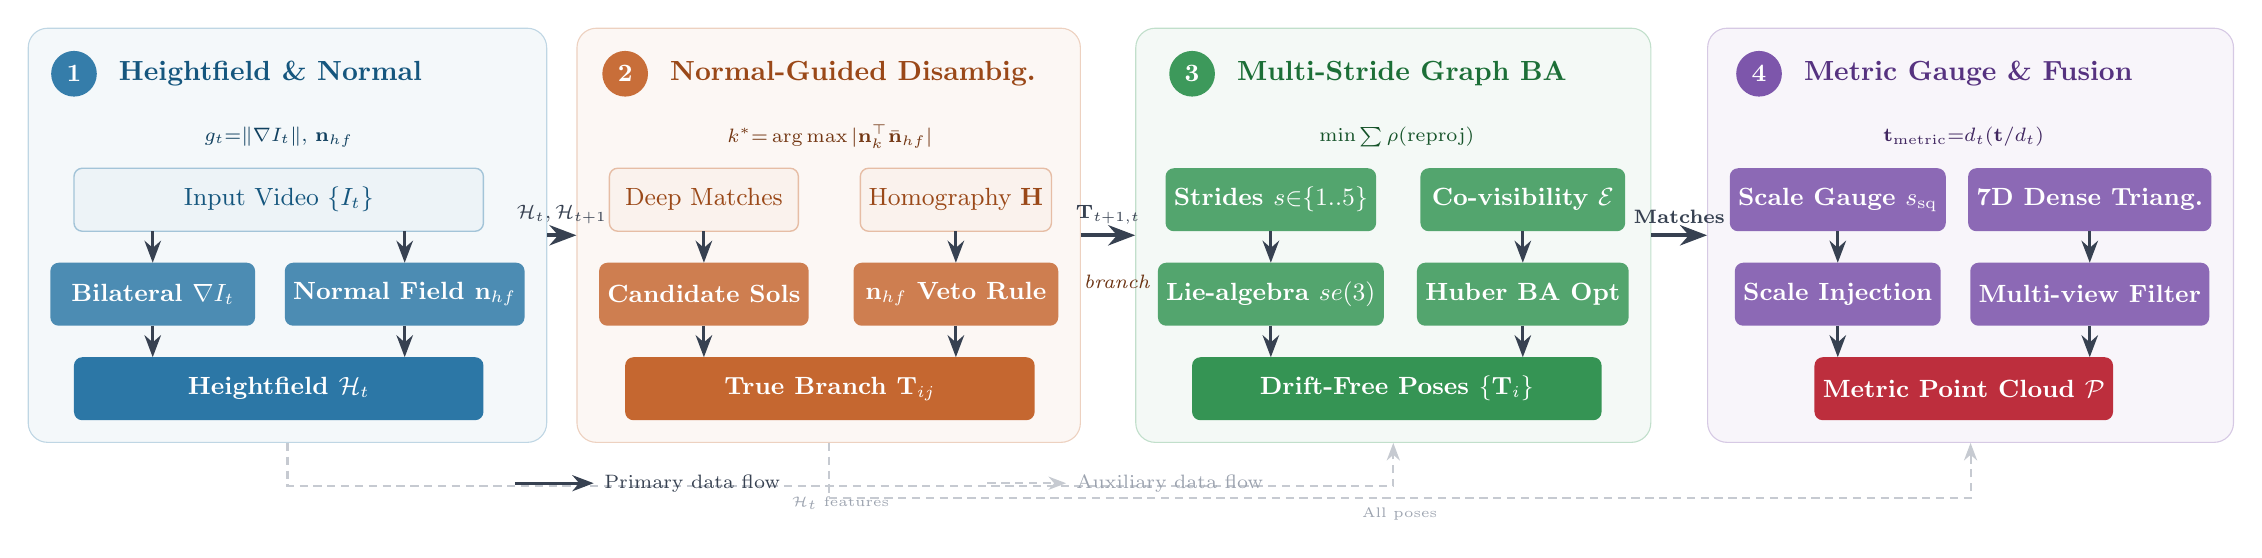
\begin{tikzpicture}[
    >=Stealth,
    % ── Box styles ──
    box/.style={rounded corners=3pt, minimum height=8.0mm, text centered,
                font=\small, inner sep=3pt, outer sep=0pt},
    ibox/.style={box, minimum width=24mm, fill=#1!8, draw=#1!40, line width=0.5pt,
                 text=#1!80!black},
    pbox/.style={box, minimum width=26mm, fill=#1!78, text=white,
                 font=\small\bfseries},
    obox/.style={box, minimum width=28mm, fill=#1!92, text=white,
                 font=\small\bfseries},
    % ── Arrow styles ──
    arr/.style={->, line width=1.1pt, color=#1},
    darr/.style={->, line width=0.75pt, color=#1!58, densely dashed},
    % ── Labels ──
    slbl/.style={font=\normalsize\bfseries, text=#1!80!black},
    numc/.style={circle, fill=#1!88, text=white, font=\small\bfseries,
                 inner sep=0pt, minimum size=5.8mm},
    annot/.style={font=\scriptsize\itshape, text=#1!55!black},
    eqtag/.style={font=\scriptsize, text=#1!60!black, align=center},
]

% ── Color palette ──
\definecolor{c1}{HTML}{1A6B9E}   % Stage 1: deep blue
\definecolor{c2}{HTML}{C05A1E}   % Stage 2: burnt orange
\definecolor{c3}{HTML}{238B45}   % Stage 3: forest green
\definecolor{c4}{HTML}{6B3FA0}   % Stage 4: royal purple
\definecolor{cout}{HTML}{B71C2C} % Output: crimson
\definecolor{carr}{HTML}{374151} % Arrows: dark gray
\definecolor{caux}{HTML}{9CA3AF} % Auxiliary: medium gray

% ═══ Grid layout: 4 stages, y-levels = header(4.3), top(2.7), mid(1.5), bot(0.3) ═══
% ═══ Stage centers at x = 0, 7.0, 14.2, 21.4                                 ═══

% ═══════════════════════════════════════════════════
%  STAGE 1 — Pseudo-3D Heightfield & Normal Construction
% ═══════════════════════════════════════════════════
\node[numc=c1] (n1) at (-2.6, 4.3) {1};
\node[slbl=c1, right=1.5mm of n1] {Heightfield \& Normal};

\node[ibox=c1, minimum width=52mm] (s1in)  at (0, 2.7) {Input Video $\{I_t\}$};
\node[pbox=c1] (s1grad) at (-1.6, 1.5) {Bilateral $\nabla I_t$};
\node[pbox=c1] (s1trunc) at (1.6, 1.5) {Normal Field $\mathbf{n}_{hf}$};
\node[obox=c1, minimum width=52mm] (s1mesh) at (0, 0.3) {Heightfield $\mathcal{H}_t$};

% Stage 1: separate orthogonal arrows (each source→target independently)
\draw[arr=carr] (s1in.south -| s1grad.north) -- (s1grad.north);
\draw[arr=carr] (s1in.south -| s1trunc.north) -- (s1trunc.north);
\draw[arr=carr] (s1grad.south) -- (s1mesh.north -| s1grad.south);
\draw[arr=carr] (s1trunc.south) -- (s1mesh.north -| s1trunc.south);

% ═══════════════════════════════════════════════════
%  STAGE 2 — Normal-Guided Disambiguation & Pose
% ═══════════════════════════════════════════════════
\node[numc=c2] (n2) at (4.4, 4.3) {2};
\node[slbl=c2, right=1.5mm of n2] {Normal-Guided Disambig.};

\node[ibox=c2] (s2mt)  at (5.4, 2.7) {Deep Matches};
\node[ibox=c2] (s2mt1) at (8.6, 2.7) {Homography $\mathbf{H}$};
\node[pbox=c2] (s2svd) at (5.4, 1.5) {Candidate Sols};
\node[pbox=c2] (s2icp) at (8.6, 1.5) {$\mathbf{n}_{hf}$ Veto Rule};
\node[obox=c2, minimum width=52mm] (s2pose) at (7.0, 0.3) {True Branch $\mathbf{T}_{ij}$};

% Stage 2: separate orthogonal arrows
\draw[arr=carr] (s2mt.south)  -- (s2svd.north);
\draw[arr=carr] (s2mt1.south) -- (s2icp.north);
\draw[arr=carr] (s2svd.south) -- (s2pose.north -| s2svd.south);
\draw[arr=carr] (s2icp.south) -- (s2pose.north -| s2icp.south);
\node[annot=c2, above right=-0.5mm and 2mm of s2icp.east] {branch veto};

% ═══════════════════════════════════════════════════
%  STAGE 3 — Multi-Stride Graph & Bundle Adjustment
% ═══════════════════════════════════════════════════
\node[numc=c3] (n3) at (11.6, 4.3) {3};
\node[slbl=c3, right=1.5mm of n3] {Multi-Stride Graph BA};

\node[pbox=c3] (s3feat) at (12.6, 2.7) {Strides $s{\in}\{1..5\}$};
\node[pbox=c3] (s3epi)  at (15.8, 2.7) {Co-visibility $\mathcal{E}$};
\node[pbox=c3] (s3xchk) at (12.6, 1.5) {Lie-algebra $\mathfrak{se}(3)$};
\node[pbox=c3] (s3dense) at (15.8, 1.5) {Huber BA Opt};
\node[obox=c3, minimum width=52mm] (s3match) at (14.2, 0.3) {Drift-Free Poses $\{\mathbf{T}_i\}$};

% Stage 3: separate orthogonal arrows
\draw[arr=carr] (s3feat.south) -- (s3xchk.north);
\draw[arr=carr] (s3epi.south)  -- (s3dense.north);
\draw[arr=carr] (s3xchk.south) -- (s3match.north -| s3xchk.south);
\draw[arr=carr] (s3dense.south) -- (s3match.north -| s3dense.south);

% ═══════════════════════════════════════════════════
%  STAGE 4 — Metric Gauge Injection & Fusion
% ═══════════════════════════════════════════════════
\node[numc=c4] (n4) at (18.8, 4.3) {4};
\node[slbl=c4, right=1.5mm of n4] {Metric Gauge \& Fusion};

\node[pbox=c4] (s4tri) at (19.8, 2.7) {Scale Gauge $s_{\mathrm{sq}}$};
\node[pbox=c4] (s4mv)  at (23.0, 2.7) {7D Dense Triang.};
\node[pbox=c4] (s4vox) at (19.8, 1.5) {Scale Injection};
\node[pbox=c4] (s4pg)  at (23.0, 1.5) {Multi-view Filter};
\node[obox=cout] (s4out) at (21.4, 0.3) {Metric Point Cloud $\mathcal{P}$};

% Stage 4: separate orthogonal arrows
\draw[arr=carr] (s4tri.south) -- (s4vox.north);
\draw[arr=carr] (s4mv.south)  -- (s4pg.north);
\draw[arr=carr] (s4vox.south) -- (s4out.north -| s4vox.south);
\draw[arr=carr] (s4pg.south)  -- (s4out.north -| s4pg.south);

% ═══════════════════════════════════════════════════
%  CORE EQUATION ANNOTATIONS
% ═══════════════════════════════════════════════════
\node[eqtag=c1] at (0, 3.5) {$g_t{=}\lVert\nabla I_t\rVert$, $\mathbf{n}_{hf}$};
\node[eqtag=c2] at (7.0, 3.5) {$k^*{=}\argmax|\mathbf{n}_k^\top\bar{\mathbf{n}}_{hf}|$};
\node[eqtag=c3] at (14.2, 3.5) {$\min\sum\rho(\text{reproj})$};
\node[eqtag=c4] at (21.4, 3.5) {$\mathbf{t}_{\mathrm{metric}}{=}d_t(\mathbf{t}/d_t)$};

% ═══════════════════════════════════════════════════
%  STAGE BACKGROUND PANELS (named, include ALL nodes)
% ═══════════════════════════════════════════════════
\begin{scope}[on background layer]
  \node[fit=(n1)(s1in)(s1grad)(s1trunc)(s1mesh), fill=c1!5, draw=c1!28,
        rounded corners=7pt, inner sep=8pt] (panel1) {};
  \node[fit=(n2)(s2mt)(s2mt1)(s2svd)(s2icp)(s2pose), fill=c2!5, draw=c2!28,
        rounded corners=7pt, inner sep=8pt] (panel2) {};
  \node[fit=(n3)(s3feat)(s3epi)(s3xchk)(s3dense)(s3match), fill=c3!5, draw=c3!28,
        rounded corners=7pt, inner sep=8pt] (panel3) {};
  \node[fit=(n4)(s4tri)(s4mv)(s4vox)(s4pg)(s4out), fill=c4!5, draw=c4!28,
        rounded corners=7pt, inner sep=8pt] (panel4) {};
\end{scope}

% ═══════════════════════════════════════════════════
%  CROSS-STAGE DATA FLOW (connect panel-to-panel borders)
% ═══════════════════════════════════════════════════
\draw[arr=carr, line width=1.5pt]
    (panel1.east) -- node[above, font=\scriptsize\bfseries, text=carr] {$\mathcal{H}_t,\mathcal{H}_{t+1}$} (panel2.west);

\draw[arr=carr, line width=1.5pt]
    (panel2.east) -- node[above, font=\scriptsize\bfseries, text=carr] {$\mathbf{T}_{t+1,t}$} (panel3.west);

\draw[arr=carr, line width=1.5pt]
    (panel3.east) -- node[above, font=\scriptsize\bfseries, text=carr] {Matches} (panel4.west);

% ═══════════════════════════════════════════════════
%  AUXILIARY DATA FLOW (dashed, routed orthogonally)
% ═══════════════════════════════════════════════════
\draw[darr=caux]
    (panel1.south) -- ++(0,-0.55) -|
    node[pos=0.25, below, font=\tiny, text=caux] {$\mathcal{H}_t$ features} (panel3.south);

\draw[darr=caux]
    (panel2.south) -- ++(0,-0.70) -|
    node[pos=0.25, below, font=\tiny, text=caux] {All poses} (panel4.south);

% ═══════════════════════════════════════════════════
%  LEGEND
% ═══════════════════════════════════════════════════
\draw[arr=carr, line width=1.05pt] (3.0, -0.90) -- (4.0, -0.90)
    node[right, font=\scriptsize, text=carr] {Primary data flow};
\draw[darr=caux] (9.0, -0.90) -- (10.0, -0.90)
    node[right, font=\scriptsize, text=caux] {Auxiliary data flow};

\end{tikzpicture}%
}%
\caption{Overview of the proposed pseudo-3D endoscopic reconstruction framework with normal-guided multi-view optimization and metric scale gauge injection.\
\textbf{Stage~1 (Heightfield and normal field construction):} bilateral gradient filtering, percentile truncation, and ROI masking generate a continuous 2.5-D heightfield mesh $\mathcal{H}_t$ and dominant physical normal field $\mathbf{n}_{hf}$.\
\textbf{Stage~2 (Normal-guided homography disambiguation):} relative planar homography $\mathbf{H}$ between frames is decomposed, and the physical camera motion branch $\mathbf{T}_{ij}$ is selected via the heightfield normal veto rule $k^* = \argmax|\mathbf{n}_k^\top \bar{\mathbf{n}}_{hf}|$, suppressing the $180^\circ$ translation flips that cheirality heuristics mis-select on a quarter of pairs.\
\textbf{Stage~3 (Multi-stride graph and bundle adjustment):} multi-stride co-visibility edges ($s \in \{1..5\}$) form closed geometric loops on $\mathrm{SE}(3)$, optimized jointly with 3D points under robust Huber loss to eliminate dead-reckoning drift.\
\textbf{Stage~4 (Metric gauge injection and dense fusion):} physical standoff distance $d_t$ injects 1:1 metric scale ($s_{\mathrm{sq}}$), followed by multi-view consistency filtering and dense point cloud fusion into $\mathcal{P}$.\
\textbf{Legend:} numbered circles denote stage index; light boxes are inputs, filled boxes are processing steps, dark boxes are outputs; solid arrows denote primary data flow; dashed arrows denote auxiliary data flow; equation annotations summarise the core operation of each stage.}
\label{fig:pipeline}
\end{figure*}

\subsection{Pseudo-3D Heightfield Mesh Construction}
\label{sec:pseudo3d}

Image gradients encode the topological structure of the surgical scene: strong gradients mark structural edges, while weak gradients from homogeneous regions are suppressed by percentile truncation.

\paragraph{Gradient computation and truncation.}
For each frame $I_t$ of spatial resolution $H \times W$ (rows $\times$ columns), we compute the gradient magnitude map $g_t(u,v) = \|\nabla I_t(u,v)\| = \sqrt{(\partial I_t/\partial u)^2 + (\partial I_t/\partial v)^2}$.
To suppress noise and spurious gradients from specular reflections, we apply percentile-based truncation: $\hat{g}_t(u,v) = g_t(u,v)$ if $g_t(u,v) \geq \tau_g$, and $0$ otherwise, where $\tau_g = \mathrm{Perc}_{\tau_{\%}}(g_t)$ denotes the $\tau_{\%}$-th percentile of the gradient distribution.
With $\tau_{\%}=68$, the upper portion of the gradient distribution is retained. The percentile is a fixed operating point, not a contribution of this paper.

\paragraph{Region-of-interest mask.}
When detectable landmarks such as a calibration pattern are present, they provide a binary region-of-interest mask $M_t(u,v) \in \{0,1\}$ (e.g., detected via standard corner detection~\cite{bradski2000opencv} for chessboard patterns).
The mask serves two purposes:
(1)~it suppresses background regions that would otherwise dominate the heightfield and corrupt ICP convergence; and
(2)~it defines the reliable region for subsequent pose quality evaluation.
The truncated gradient map is masked as $\tilde{g}_t(u,v) = \hat{g}_t(u,v) \cdot M_t(u,v)$.
This masking ensures that only gradient responses within the region of interest contribute to the heightfield, removing the influence of irrelevant tissue and instrument regions.
The interface is deliberately source-agnostic: $M_t$ may come from a chessboard hull, a contour fallback, or a semantic tissue probability in $[0,1]$. Instruments and specular blobs should be excluded from the tissue heightfield rather than reconstructed as a second depth layer, which a single 2.5-D mesh cannot represent.

\paragraph{Heightfield mesh generation.}
The masked gradient map $\tilde{g}_t$ (normalised to $[0,255]$) is lifted to a 2.5-D heightfield mesh $\mathcal{H}_t$ by constructing a regular grid with cell size $c_{\mathrm{cell}}$ pixels (default: 3).
Each grid vertex $(u,v)$ is assigned a height value $h(u,v) = z_s \cdot \tilde{g}_t(u,v) / 255$, where $z_s = 0.15\,\max(H,W)$ is the height scaling factor so that the maximum height is comparable to image dimensions for numerical stability.
Adjacent vertices are connected via a regular grid triangulation, yielding a manifold surface $\mathcal{H}_t = (\mathcal{V}_t, \mathcal{F}_t)$ with $|\mathcal{V}_t| \approx HW / c_{\mathrm{cell}}^2$ vertices.

\paragraph{Physical surface normal field.}
In addition to height coordinates, each vertex $(u,v)$ on the triangular mesh defines a continuous surface normal $\mathbf{n}(u,v)$ computed from adjacent facet normals:
\begin{equation}
    \mathbf{n}_{hf}(u,v) = \frac{\sum_{j \in \mathcal{F}(u,v)} \mathbf{n}_j}{\left\|\sum_{j \in \mathcal{F}(u,v)} \mathbf{n}_j\right\|_2},
    \label{eq:normal_field}
\end{equation}
where $\mathcal{F}(u,v)$ denotes the set of triangular facets sharing vertex $(u,v)$, and $\mathbf{n}_j$ is the cross-product normal of facet $j$.
In surgical cavities and anatomical phantom setups, the camera optical axis maintains a consistent viewing inclination relative to the underlying tissue bed.
The dominant orientation $\bar{\mathbf{n}}_{hf} = \mathrm{median}_{(u,v)} \mathbf{n}_{hf}(u,v)$ serves as an operative physical normal prior that constrains inter-frame geometry.

\subsection{Normal-Guided Planar Homography Disambiguation}
\label{sec:homography_disambiguation}
\label{sec:registration}

When endoscopic cameras observe planar surgical phantoms, liver surfaces, or anatomical planes, points on a planar structure $\mathbf{n}^\top \mathbf{X} = d$ transform between views $i$ and $j$ via a homography matrix $\mathbf{H} \in \mathbb{R}^{3 \times 3}$:
\begin{equation}
    \mathbf{p}_j \sim \mathbf{H}\,\mathbf{p}_i, \quad
    \mathbf{H} = \mathbf{K} \left( \mathbf{R}_{ij} + \frac{\mathbf{t}_{ij}}{d_i}\mathbf{n}_i^\top \right) \mathbf{K}^{-1},
    \label{eq:homography_formula}
\end{equation}
where $\mathbf{R}_{ij} \in \mathrm{SO}(3)$ is the relative rotation, $\mathbf{t}_{ij} \in \mathbb{R}^3$ is the translation vector, $\mathbf{n}_i$ is the unit surface normal in the reference camera frame, and $d_i$ is the orthogonal distance from camera $i$ to the plane.
The normalized homography $\tilde{\mathbf{H}} = \mathbf{K}^{-1} \mathbf{H} \mathbf{K}$ is estimated from robust feature correspondences (e.g., deep LoFTR matches or SIFT) via RANSAC.

\paragraph{The two-fold physical ambiguity.}
Analytical decomposition of $\tilde{\mathbf{H}}$ via singular value decomposition~\cite{malis2007deeper} yields four mathematical solutions, of which exactly two satisfy the positive cheirality constraint, denoted as physical candidates $\mathcal{S}_1 = (\mathbf{R}_1, \mathbf{t}_1/d, \mathbf{n}_1)$ and $\mathcal{S}_2 = (\mathbf{R}_2, \mathbf{t}_2/d, \mathbf{n}_2)$.
Under narrow baselines typical of endoscopic videos ($\|\mathbf{t}\| \ll d$), both solutions yield almost identical reprojection errors on image features:
$\|\mathbf{p}_j - \pi(\mathbf{H}_1 \mathbf{p}_i)\| \approx \|\mathbf{p}_j - \pi(\mathbf{H}_2 \mathbf{p}_i)\| < 1.0\,\mathrm{px}$.
Standard heuristic rules---such as selecting the solution with the largest number of positive triangulated points or the minimal rotation---frequently fail, choosing an unnatural fronto-parallel branch where the estimated translation vector is reversed or biased by $90^\circ$.
On our chessboard benchmark the max-cheirality heuristic mis-selects the reference-consistent branch on $24$--$33\%$ of frame pairs (Supplementary Material, Section~I).

\paragraph{Heightfield normal veto.}
We resolve this ambiguity by evaluating the directional alignment between the candidate plane normals $\{\mathbf{n}_1, \mathbf{n}_2\}$ and the physical surface normal prior $\bar{\mathbf{n}}_{hf}$ derived from the pseudo-3D heightfield mesh (Eq.~\eqref{eq:normal_field}):
\begin{equation}
    k^* = \argmax_{k \in \{1, 2\}} \left| \mathbf{n}_k^\top \bar{\mathbf{n}}_{hf} \right|.
    \label{eq:normal_veto}
\end{equation}
The selected solution $(\mathbf{R}_{k^*}, \mathbf{t}_{k^*}, \mathbf{n}_{k^*})$ is the branch whose plane normal agrees with the physical inclination of the operative surface.
Measured against the reference-consistent branch on the chessboard benchmark, the veto selects the correct branch on $75.5\%$ of adjacent pairs and $73.8\%$ of stride-8 pairs, exceeding the cheirality heuristic on wide-stride pairs ($69.0\%$), where the baseline is larger and the two branches are most separable (Supplementary Material, Section~I).
The veto requires no external pose sensor; residual pair-level branch errors are transient outliers for the multi-stride bundle adjustment of Section~\ref{sec:multistride_ba}, which optimises over loops rather than trusting any single decomposition.

\subsection{Multi-Stride Co-Visibility Graph and Joint Bundle Adjustment}
\label{sec:multistride_ba}

Conventional monocular visual odometry integrates relative poses in a sequential Markovian chain ($\mathbf{T}_{0 \to t} = \prod_{k=0}^{t-1} \mathbf{T}_{k \to k+1}$), which causes compounding dead-reckoning drift over extended sequences.
To overcome this, we construct a \emph{multi-stride co-visibility graph} and optimize camera poses and 3D scene points jointly via non-linear Bundle Adjustment.

\paragraph{Multi-stride graph construction.}
Given $N$ keyframes, we establish co-visibility edges across multi-frame temporal skips: $\mathcal{E} = \{ (i, j) \mid 1 \leq j - i \leq S_{\max}, \; 0 \leq i < j < N \}$, where $S_{\max} \in \{3, 4, 5\}$ is the maximum co-visibility stride.
For each edge $(i, j) \in \mathcal{E}$, deep correspondences $\mathcal{M}_{ij} = \{(\mathbf{u}_i^{(m)}, \mathbf{u}_j^{(m)})\}$ are extracted using LoFTR~\cite{sun2021loftr} and filtered via homography RANSAC.
Multi-view tracks are formed by chaining pairwise matches across overlapping frames, and initial 3D point positions $\mathbf{X}_k \in \mathbb{R}^3$ are triangulated via multi-view linear SVD.

\paragraph{Lie-algebra bundle adjustment formulation.}
We parameterize each camera pose $\mathbf{T}_i \in \mathrm{SE}(3)$ (world-to-camera) using $\mathfrak{se}(3)$ Lie-algebra twist coordinates $\boldsymbol{\xi}_i = (\boldsymbol{\omega}_i^\top, \boldsymbol{\upsilon}_i^\top)^\top \in \mathbb{R}^6$ via the exponential map:
\begin{equation}
    \mathbf{T}_i = \exp\left(\boldsymbol{\xi}_i^\wedge\right) = \begin{bmatrix} \exp(\boldsymbol{\omega}_i^\wedge) & \mathbf{V}(\boldsymbol{\omega}_i)\boldsymbol{\upsilon}_i \\ \mathbf{0}^\top & 1 \end{bmatrix},
    \label{eq:se3_exp}
\end{equation}
where $\exp(\boldsymbol{\omega}^\wedge)$ is the Rodrigues rotation and $\mathbf{V}(\boldsymbol{\omega}) = \mathbf{I} + \frac{1-\cos\theta}{\theta^2}\boldsymbol{\omega}^\wedge + \frac{\theta - \sin\theta}{\theta^3}(\boldsymbol{\omega}^\wedge)^2$ with $\theta = \|\boldsymbol{\omega}\|$ is the left $\mathrm{SO}(3)$ Jacobian, with the first camera fixed at the world origin ($\boldsymbol{\xi}_0 = \mathbf{0}$).
The joint objective over all free camera poses $\{\boldsymbol{\xi}_i\}_{i=1}^{N-1}$ and 3D scene points $\{\mathbf{X}_k\}_{k=1}^{K}$ is formulated as:
\begin{equation}
    \min_{\{\boldsymbol{\xi}_i\}, \{\mathbf{X}_k\}} \sum_{(i, k) \in \mathcal{O}} \rho_{\mathrm{Huber}}\!\left(\left\|\mathbf{u}_{i,k} - \pi\!\left(\mathbf{K} \exp(\boldsymbol{\xi}_i^\wedge)\mathbf{X}_k\right)\right\|_2\right) + \lambda_{\mathrm{cheir}} \sum_{(i, k) \in \mathcal{O}} \max\left(0, d_{\min} - z_{i,k}\right)^2,
    \label{eq:ba_objective}
\end{equation}
where $\mathcal{O}$ is the set of all 2D-3D observation pairs, $\rho_{\mathrm{Huber}}(\cdot)$ is the robust Huber penalty with threshold $\delta_H = 3.0\,\mathrm{px}$, $z_{i,k} = [\exp(\boldsymbol{\xi}_i^\wedge)\mathbf{X}_k]_z$ is the depth in camera frame $i$, and the second term enforces a positive cheirality safety barrier ($d_{\min} = 10.0\,\mathrm{mm}$).
The objective is optimized on GPU via AdamW with cosine learning rate annealing, converging in 400--800 iterations.
Because edges span across multi-frame skips, the resulting graph forms dense triangle and polygon closures that distribute local tracking errors and eliminate trajectory drift.

\subsection{Metric Scale Gauge Injection}
\label{sec:metric_gauge}

Monocular reconstruction from visual correspondences is fundamentally scale-ambiguous: the translation vector recovered from homography or essential matrix decomposition represents a dimensionless ratio $\hat{\mathbf{t}} = \mathbf{t} / d$.
Feed-forward models (such as VGGT and DUSt3R) predict scale-less geometry that wanders by orders of magnitude across sequences ($10\times$--$647\times$).

\paragraph{Physical scale recovery.}
When a physical reference of known pitch $s_{\mathrm{sq}}$ (e.g., standard $3.0$\,mm calibration squares or surgical fiducials) is visible in the endoscopic field of view, we inject an exact physical metric gauge.
Let $p_{\mathrm{sq}}$ be the measured pixel pitch of adjacent pattern corners, and $f = (f_x + f_y)/2$ the focal length in pixels. The absolute working standoff distance $d_t$ to the operative surface is determined by $d_t = f \cdot s_{\mathrm{sq}} / p_{\mathrm{sq}}$, and the dimensionless translation vector is scaled to physical millimetres via $\mathbf{t}_{\mathrm{metric}} = d_t \cdot (\mathbf{t}/d_t)$.

\paragraph{Sparse vs.\ full gauge propagation.}
In practice, full physical targets may not be visible in every surgical frame.
Our framework supports two operating modes:
\begin{itemize}[noitemsep]
    \item \textbf{Sparse Gauge Mode}: The metric gauge is anchored on a sparse subset of keyframes (e.g., every 10th frame, or only when the pattern is fully unoccluded). The metric scale is then propagated to all intermediate frames through the multi-stride bundle adjustment graph (Section~\ref{sec:multistride_ba}). On the 17-sequence benchmark the propagated scale stays within $0.55\times$--$2.44\times$ of the reference (median $1.46\times$): markedly better than unconstrained feed-forward drift ($95\times$--$2295\times$), but not a substitute for full gauge coverage.
    \item \textbf{Full Gauge Mode}: When the pattern is visible across the recording, every frame is gauge-referenced. The reported trajectory is then the per-frame gauge solution itself, evaluated against an independent stereo-verified PnP reference; it attains the pattern-reference floor of $4.49$\,mm median ATE. This mode measures the metric accuracy ceiling available to the framework, not the visual front-end's pattern-free tracking error (which is reported separately as Ours-BA).
\end{itemize}

\subsection{Dense Epipolar Matching and Multi-Frame Fusion}
\label{sec:epipolar}

To reconstruct a \emph{dense} point cloud beyond sparse landmarks or feature tracks, we establish pixel-level correspondences between frames using heightfield-based geometric feature matching with epipolar constraints.

\paragraph{7D geometric feature extraction.}
For each valid grid point on the heightfield, we construct a 7-dimensional feature vector:
\begin{equation}
    \mathbf{f}(u,v) = \bigl[\,\underbrace{\tfrac{u}{W},\; \tfrac{v}{H}}_{\text{position}},\; \underbrace{\tfrac{h}{z_s}}_{\text{height}},\; \underbrace{\tfrac{n_x}{\|\mathbf{n}\|},\; \tfrac{n_y}{\|\mathbf{n}\|},\; \tfrac{n_z}{\|\mathbf{n}\|}}_{\text{normal}},\; \underbrace{\tfrac{c}{255}}_{\text{color}}\,\bigr]^\top,
    \label{eq:feature}
\end{equation}
combining normalized position $(u/W, v/H)$, height $h/z_s$, surface normal $(n_x,n_y,n_z)^\top/\|\mathbf{n}\|$, and colour $c/255$ (where $c \in [0,255]$ is the grey-scale intensity at the vertex).
The surface normal is estimated from the heightfield via finite differences, providing geometric context that disambiguates repetitive texture patterns.

\paragraph{RT-predicted search window.}
Given the estimated relative transformation $\mathbf{T}_{t+1,t}$ from Section~\ref{sec:registration}, which is defined in the heightfield space, we predict the location of each source grid point in the target frame via $[u', v', h', 1]^\top = \mathbf{T}_{t+1,t} [u, v, h, 1]^\top$, where $(u,v,h)$ is the source vertex height and $(u',v',h')$ its predicted counterpart.
This provides a tight search prior that reduces the matching search space from the full image to a local window of radius $r$ (default: $r{=}25$ pixels) around the predicted location.

\paragraph{Epipolar constraint.}
For frames with known camera intrinsics and estimated pose, we compute the fundamental matrix $\mathbf{F} = \mathbf{K}^{-\top}[\mathbf{t}]_\times \mathbf{R}\,\mathbf{K}^{-1}$, where $\mathbf{R}$ and $\mathbf{t}$ are the relative rotation and translation and $[\mathbf{t}]_\times$ is the skew-symmetric matrix of $\mathbf{t}$, and enforce the epipolar band constraint $|\mathbf{u}'^\top \mathbf{F}\, \mathbf{u}| < \epsilon_{\mathrm{epi}}$ (with $\epsilon_{\mathrm{epi}} = 2.0$\,px), where $\mathbf{u},\mathbf{u}'$ are homogeneous pixel coordinates.
This geometric constraint reduces false matches caused by repetitive texture patterns prevalent in endoscopic scenes.

\paragraph{Feature matching with cross-check.}
Within the search window, correspondences are established by minimizing the $\ell_2$ feature distance $k^* = \argmin_{k \in W_r} \|\mathbf{f}(u,v) - \mathbf{f}(u_k,v_k)\|_2$ subject to the epipolar constraint.
A cross-check (reverse match consistency within 3\,px) rejects asymmetric matches, and a depth consistency filter removes points with depth exceeding $5\times$ the median depth.

\paragraph{Multi-frame metric fusion.}
\label{sec:fusion}

The dense correspondences from each frame pair are triangulated into 3D points using the camera intrinsics and poses, then fused across all frames.

\paragraph{Triangulation.}
Given matched homogeneous pixel coordinates $(\mathbf{u}_i, \mathbf{u}_j)$ in frames $i$ and $j$, the 3D point is obtained by linear triangulation of the two projection matrices $\mathbf{P}_i = \mathbf{K}[\mathbf{I}\,|\,\mathbf{0}]$ and $\mathbf{P}_j = \mathbf{K}[\mathbf{R}\,|\,\mathbf{t}]$:
\begin{equation}
    \tilde{\mathbf{X}}_k = \argmin_{\tilde{\mathbf{X}}} \|\mathbf{A}\tilde{\mathbf{X}}\|^2, \quad
    \mathbf{A} = \begin{bmatrix}
        [\mathbf{u}_i]_\times \mathbf{P}_i \\
        [\mathbf{u}_j]_\times \mathbf{P}_j
    \end{bmatrix},
    \label{eq:triangulate}
\end{equation}
solved via SVD, where $\tilde{\mathbf{X}}$ is homogeneous, $[\mathbf{u}]_\times$ is the $3{\times}3$ skew-symmetric matrix of $\mathbf{u}$, and the metric point is $\mathbf{X}_k$ after dehomogenisation.
Points with reprojection error exceeding $\tau_{\mathrm{reproj}} = 2.0\,\mathrm{px}$ in either view are discarded.

\paragraph{Multi-view consistency.}
A triangulated 3D point $\mathbf{X}_k$ is retained only if it is consistent in at least two of its observing views: $\frac{1}{|\mathcal{V}|} \sum_{m \in \mathcal{V}} \mathbb{1}[\|\pi(\mathbf{K}\mathbf{T}_m\mathbf{X}_k) - \mathbf{u}_{m,k}\| < \tau_{\mathrm{reproj}}] \geq \frac{2}{|\mathcal{V}|}$, where $\mathcal{V}$ is the set of views observing $\mathbf{X}_k$, $\mathbf{T}_m$ is the pose of view $m$, $\mathbf{u}_{m,k}$ is the observed pixel, $\pi(\cdot)$ is perspective projection, and $\mathbb{1}[\cdot]$ is the indicator function.
This multi-view check removes spurious outliers from specular highlights.

\paragraph{Voxel-grid deduplication.}
Overlapping reconstructions from adjacent frame pairs produce duplicate points.
We apply voxel-grid downsampling (resolution: 1.0\,mm) that averages positions and colors within each voxel, followed by statistical outlier removal ($k{=}20$ neighbors, $2.0\sigma$ threshold), yielding the final fused point cloud $\mathcal{P}$.

\paragraph{Complexity analysis.}
The per-frame computational cost is dominated by ICP registration ($O(|\mathcal{V}| \log |\mathcal{V}|)$ per iteration with a KD-tree) and dense matching ($O(K_{\mathrm{samp}} \cdot r^2)$, where $K_{\mathrm{samp}} = HW / c_{\mathrm{cell}}^2$ is the number of sampled grid points and $r$ is the search radius).
With the default parameters, the pipeline processes each frame pair in approximately 1.2\,s on a single CPU core, making it suitable for offline surgical analysis.

\subsection{Calibrated End-to-End Stereo Variant}
\label{sec:e2e_stereo}

The classical pipeline of Sections~\ref{sec:pseudo3d}--\ref{sec:fusion} derives its heightfield from image gradients and estimates pose through ICP on these pseudo-3D surfaces. The gradient-based heightfield is a \emph{proxy} for true scene geometry: it encodes edge structure rather than metric depth, and its accuracy is bounded by the gradient signal in texture-poor tissue. This section describes an optional extension used only when stereo imaging hardware is available. A learned disparity estimate replaces the gradient-derived height, and the heightfield then refines rather than replaces that metric depth. Depth results are reported in Table~\ref{tab:sota_depth}.

\paragraph{Problem formulation.}
Given a rectified stereo pair $(I_l, I_r)$ with known intrinsics $\mathbf{K}$ (focal length $f_x$ along the disparity direction) and baseline $b$, the metric depth $d(u,v)$ at pixel $(u,v)$ relates to the disparity $d_{\mathrm{disp}}(u,v)$ by the pinhole triangulation:
\begin{equation}
    d(u,v) = \frac{f_x \, b}{d_{\mathrm{disp}}(u,v)}.
    \label{eq:stereo_depth}
\end{equation}
The key challenge is estimating a dense, sub-pixel disparity field that is robust to the weak texture, specular reflections, and non-Lambertian surfaces typical of endoscopic tissue. We address this with a differentiable stereo network whose disparity output is (i)~converted to metric depth via~\eqref{eq:stereo_depth}, (ii)~lifted to a heightfield that inherits the geometric structure of the classical pipeline, and (iii)~used jointly with the heightfield for pose estimation. The three modules are trained end-to-end so that the disparity head is optimised not only for depth accuracy but also for the downstream geometric consistency that the heightfield and pose modules require.

\paragraph{Encoder with attention.}
Each image is encoded by a ResNet-based backbone with BasicBlock stages producing multi-scale features $\{\boldsymbol{\Phi}^{(s)}\}_{s=1}^{S}$ at $S$ resolutions (written $\boldsymbol{\Phi}$ rather than $\mathbf{F}$ to avoid collision with the fundamental matrix). A Convolutional Block Attention Module (CBAM)~\cite{woo2018cbam} refines each stage, applying channel attention followed by spatial attention:
\begin{equation}
    \boldsymbol{\Phi}'^{(s)} = \mathrm{CA}(\boldsymbol{\Phi}^{(s)}) \otimes \boldsymbol{\Phi}^{(s)}, \qquad
    \boldsymbol{\Phi}''^{(s)} = \mathrm{SA}(\boldsymbol{\Phi}'^{(s)}) \otimes \boldsymbol{\Phi}'^{(s)},
    \label{eq:cbam}
\end{equation}
where $\mathrm{CA}(\cdot) = \sigma(\mathrm{MLP}(\mathrm{GAP}(\cdot)+\mathrm{GMP}(\cdot)))$ pools across spatial dimensions to re-weight channels (GAP/GMP: global average/max pooling, $\sigma$: sigmoid, MLP: shared two-layer perceptron), and $\mathrm{SA}(\cdot) = \sigma(f^{7\times7}([\mathrm{GAP};\mathrm{GMP}]))$ pools across channels to re-weight spatial locations ($f^{7\times7}$: $7{\times}7$ convolution, $[\cdot;\cdot]$: channel concatenation). Channel attention suppresses uninformative feature channels (e.g., those dominated by specular highlights), while spatial attention focuses on structurally informative regions, both important in endoscopic imagery where illumination is highly non-uniform. The encoded features are aggregated to a single feature volume $\boldsymbol{\Phi}_l, \boldsymbol{\Phi}_r$ at the highest resolution.

\paragraph{Differentiable cost-volume aggregation.}
Stereo cost aggregation constructs a 3D cost volume $\mathbf{C} \in \mathbb{R}^{D \times H \times W}$ by shifting the right feature map across $D$ disparity hypotheses and computing a per-pixel, per-disparity matching cost as the channel-wise mean of the element-wise product of the left and shifted-right feature vectors:
\begin{equation}
    \mathbf{C}(d, u, v) = \frac{1}{C}\sum_{c=1}^{C} \boldsymbol{\Phi}_l^{(c)}(u, v)\, \boldsymbol{\Phi}_r^{(c)}(u - d, v),
    \label{eq:costvol}
\end{equation}
where $C$ is the feature-channel count and $\boldsymbol{\Phi}^{(c)}$ denotes the $c$-th channel; the variant V4 instead forms the cost from group-wise correlation~\cite{guo2019gwcnet}. The raw cost volume is regularised by a cascade of 3D convolutions~\cite{chang2018psmnet} operating over the joint spatial--disparity space, which enforces disparity smoothness while preserving depth discontinuities at tissue boundaries. This 3D aggregation is essential because 2D convolutions cannot propagate evidence along the disparity axis and therefore produce fuzzy edges in low-texture regions. A final regressor converts the regularised volume to a sub-pixel disparity map $\hat{d}_{\mathrm{disp}}$.

\paragraph{Heightfield head and joint pose.}
The predicted disparity $\hat{d}_{\mathrm{disp}}$ is converted to metric depth $\hat{d}(u,v)$ via~\eqref{eq:stereo_depth} and lifted to a heightfield $\hat{\mathcal{H}}_t$ using the same grid construction as Section~\ref{sec:pseudo3d}, with the learned depth replacing the gradient proxy via $\hat{h}(u,v) = z_s \cdot (\hat{d}(u,v) - \min\hat{d}) / (\max\hat{d} - \min\hat{d})$.
A pose-estimation head consumes the left--right features jointly with the heightfield to predict the relative transformation $\mathbf{T}_{t+1,t}$, replacing the ICP refinement when the network is used end-to-end. The three losses are combined: $\mathcal{L} = \lambda_d \mathcal{L}_{\mathrm{disp}} + \lambda_h \mathcal{L}_{\mathrm{height}} + \lambda_p \mathcal{L}_{\mathrm{pose}}$, where $\lambda_d, \lambda_h, \lambda_p$ are scalar loss weights (default $\lambda_d{=}1.0,\lambda_h{=}0.1,\lambda_p{=}0.5$), $\mathcal{L}_{\mathrm{disp}}$ is a smooth-$L_1$ disparity loss against stereo ground truth, $\mathcal{L}_{\mathrm{height}}$ is an $L_2$ heightfield (shape) loss against the pseudo-3D target, and $\mathcal{L}_{\mathrm{pose}}$ is a geodesic pose loss~\cite{wang2019densefusion}. Joint optimisation couples disparity accuracy with geometric consistency: the heightfield and pose losses regularise the disparity toward configurations that yield well-conditioned 3D structure, which is exactly the property the classical pipeline relies upon for ICP convergence. Architectural variants V2--V4 differ in the encoder (custom vs.\ pretrained ResNet) and cost-volume construction (channel-wise dot-product vs.\ group-wise correlation~\cite{guo2019gwcnet}); their detailed ablation is reported in Supplementary Material, Section~E.

\paragraph{Relationship to the classical pipeline.}
The two formulations are complementary. The classical pipeline (Sections~\ref{sec:pseudo3d}--\ref{sec:fusion}) is calibration-free and operates from monocular gradients, making it applicable to legacy footage and uncalibrated sequences, but its heightfield is a structural proxy rather than metric depth. The end-to-end variant requires a calibrated stereo pair and a training set, but yields metric depth whose accuracy is no longer bounded by gradient quality. The pseudo-3D heightfield is retained in both: in the classical case it is the primary geometric signal, and in the learned case it is the interface through which the disparity is regularised for 3D consistency. This shared heightfield representation is what allows the ICP and dense-matching modules of Section~\ref{sec:registration} to be reused without modification.





\section{Experiments}
\label{sec:experiments}

\subsection{Dataset and Evaluation Protocol}
\label{sec:dataset}

\paragraph{Dataset.}
We evaluate all methods on an endoscopic chessboard sequence of 100 frames captured with a Karl Storz laparoscopic camera at a native resolution of $1280 \times 720$, under endoscopic imaging conditions including specular reflections, partial occlusion by surgical instruments, and non-rigid tissue deformation.
For our classical pipeline the frames are downsampled by a factor of two to $640 \times 358$ to bound the per-frame computational cost, and the camera matrix used internally is the image-diagonal estimate $f_x = f_y = \sqrt{640^2 + 358^2} \approx 733.3\,\mathrm{px}$ with the principal point at the image centre; the depth and pose evaluation, however, is performed at the native $1280 \times 720$ resolution using the calibrated intrinsics ($f_x = f_y = 2304\,\mathrm{px}$, principal point at image centre), so that the ground-truth corner depths and the \texttt{solvePnP} pose reference are as accurate as possible.
The chessboard marker has $8 \times 5$ inner corners (40 points) with square side length $s_{\mathrm{sq}} = 5.0\,\mathrm{mm}$, providing the independent pose reference via \texttt{solvePnP} (reprojection RMSE $< 0.5\,\mathrm{px}$) used only for evaluation, not as an input to our pipeline.

\paragraph{Input protocol.}
Each method takes the same 50 frames (the first 50 frames of the 100-frame sequence) as input, producing:
(1)~a 3D point cloud representing the reconstructed scene; and
(2)~estimated camera poses; for our method the poses are estimated internally by the heightfield-ICP pipeline of Section~\ref{sec:registration} (not supplied as ground truth), whereas the baselines estimate poses with their own front-ends.

\paragraph{Evaluation metrics.}
We adopt six complementary metrics spanning geometric quality and pose accuracy:
\begin{itemize}[noitemsep]
    \item \textbf{PCA shape ratio} ($\lambda_3/\lambda_1$): Ratio of the smallest to largest eigenvalue of the point cloud's covariance matrix $\mathbf{C} = \frac{1}{K}\sum_{k} (\mathbf{X}_k - \bar{\mathbf{X}})(\mathbf{X}_k - \bar{\mathbf{X}})^\top$.
    A well-distributed 3D structure satisfies $\lambda_3/\lambda_1 \geq 0.25$; values below indicate degenerate geometry.
    \item \textbf{Shape classification}: Normal\,3D ($\lambda_3/\lambda_1 \geq 0.25$), Flat ($0.15 \leq \lambda_3/\lambda_1 < 0.25$), Cone ($\lambda_3/\lambda_1 < 0.15$). This threshold is chosen so that a Normal\,3D point cloud has comparable extent along all three principal axes, which is the minimum requirement for representing a 3D surgical scene.
    \item \textbf{ATE} (Absolute Trajectory Error)~\cite{sturm2012benchmark}: RMSE of camera positions after Sim3 alignment (scale, rotation, translation) between estimated and ground-truth trajectories.
    \item \textbf{RPE} (Relative Pose Error): Mean relative translation error between consecutive frame pairs, measuring local consistency independent of global drift. A global rotation error is not reported: the benchmark sequence is translation-dominant (reference relative rotation ${\approx}0.3^{\circ}$ per frame), so the rotational part of a position-fitted Sim3 alignment is ill-conditioned.
    \item \textbf{Sim3 scale factor}: The scale component of the Sim3 alignment; $1.0\times$ indicates correct metric scale.
    \item \textbf{Depth metrics}: absolute relative error (AbsRel), root-mean-square error (RMSE), and threshold accuracy ($\delta_1$), computed at chessboard corner positions after affine alignment ($\text{gt} = a{\cdot}\text{pred}+b$), measuring per-point depth accuracy against PnP-derived ground truth. The affine (scale$+$shift) alignment is used here, rather than the median-scale alignment adopted on the public stereo datasets (Sections~\ref{sec:endonerf}--\ref{sec:stereo_lap}), because the chessboard ground truth is PnP-derived and the heightfield/SGM disparity is a structural proxy whose systematic offset must be removed before the per-corner error is meaningful; the chessboard depth figures are therefore not comparable in magnitude with the other datasets, only within this table.
\end{itemize}

\subsection{Compared Methods}
\label{sec:compared_methods}

We compare against eight representative baselines spanning classical SfM, feed-forward 3D reconstruction networks, and pose regression:

\begin{itemize}[noitemsep]
    \item \textbf{Stereo SGM}: Semi-global matching (SGM)~\cite{hirschmuller2008sgm} stereo pipeline with the same heightfield-ICP poses as Ours, serving as a classical stereo baseline with identical pose input.
    \item \textbf{ORB-SfM}~\cite{mur2015orbslam}: ORB feature extraction~\cite{rublee2011orb} with 5-point essential matrix estimation~\cite{nister2004efficient} and incremental pose chaining via \texttt{recoverPose}. Triangulation via \texttt{triangulatePoints}. No bundle adjustment.
    \item \textbf{COLMAP}~\cite{schoenberger2016sfm}: SIFT features~\cite{lowe2004distinctive} with incremental SfM and full bundle adjustment. A well-established classical baseline.
    \item \textbf{VGGT}~\cite{wang2025vggt} (CVPR 2025 Best Paper): Feed-forward Vision Geometry Grounded Transformer that jointly predicts camera poses, depth maps, and 3D point clouds from an image sequence in a single forward pass. DINOv2~\cite{oquab2023dinov2} backbone with 1.2B parameters.
    \item \textbf{Reloc3R}~\cite{dong2025reloc3r} (CVPR 2025): Relative pose regression network with motion averaging for global pose estimation. Extends DUSt3R for camera relocalization. Outputs poses only (no point cloud).
    \item \textbf{DUSt3R}~\cite{wang2024dust3r} (CVPR 2024): Dense uncalibrated stereo 3D reconstruction via paired pointmap prediction and global alignment optimization (Levenberg--Marquardt).
    \item \textbf{MASt3R}~\cite{leroy2024mast3r} (ECCV 2024): Extension of DUSt3R with local feature matching and metric pointmaps for improved 3D reconstruction and camera pose estimation.
    \item \textbf{MUSt3R}~\cite{cabon2025must3r} (CVPR 2025): Multi-view extension of DUSt3R that processes $N{>}2$ views simultaneously with a memory network, producing globally consistent pointmaps and poses without pairwise alignment.
\end{itemize}

\paragraph{Implementation details.}
All methods use the same 50 input frames (the first 50 frames of the 100-frame sequence) with default hyperparameters and their officially released pretrained models; each method resizes the frames to its own operating resolution (our pipeline to $640{\times}358$, MUSt3R to $224{\times}224$, and the other feed-forward networks to their native input sizes), so the comparison is on the same image content rather than on identical pixel grids.
No method receives camera intrinsics as input (except ORB-SfM, which uses the chessboard-calibrated intrinsics for \texttt{recoverPose}).
Ours estimates camera poses internally by registering consecutive heightfield meshes with FPFH features, RANSAC, and point-to-point ICP (Section~\ref{sec:registration}); the chessboard is used only to obtain intrinsics and an independent pose reference for evaluation.
DUSt3R and MASt3R are run with the global alignment optimizer (pairwise then global refinement).
VGGT processes 50 frames with sub-sequence windowing (8 frames per window).
MUSt3R uses a memory network with 8 keyframes at $224{\times}224$ resolution.
For our method, we use the following parameters: gradient threshold $\tau_{\%}=68$, mesh cell size $c_{\mathrm{cell}}=3$, coarse alignment via PCA principal-axis alignment followed (on failure) by FPFH-feature-matched RANSAC with a $5\times$-enlarged correspondence distance, refinement via point-to-point ICP with an adaptive (scale-derived) correspondence distance, dense matching search radius $r{=}25$, and epipolar band $\epsilon_{\mathrm{epi}}=2.0$.
The evaluation uses a fixed random seed (42) for reproducibility of the PCA sub-sampling step.
Complete hyperparameter and hardware details are provided in the Supplementary Material, Section~A.

\subsection{Quantitative Results}
\label{sec:results}

% ── Comprehensive chessboard comparison table (auto-generated) ──
\begin{table*}[tbp]
\centering
\caption{
  Comparison on the endoscopic chessboard benchmark (100 frames captured at $1280{\times}720$, 50 used as input; our pipeline runs on $640{\times}358$ downsampled frames, Karl Storz laparoscope).
  Depth metrics (AbsRel, RMSE, $\delta_1$) computed at chessboard corners (40 per frame, 4000 total, ground-truth depth range 225--784\,mm) after affine alignment ($\text{gt}=a{\cdot}\text{pred}+b$); the RMSE values are therefore in millimetres against depths of several hundred millimetres, so an RMSE of, e.g., 109\,mm corresponds to a relative error of about 22\%, consistent with the reported AbsRel.
  $\lambda_3/\lambda_1$: 3D shape ratio (${\geq}0.25$ Normal\,3D; 0.15--0.25 Flat; ${<}0.15$ Cone).
  ATE (mm) and Sim3 scale are computed against the independent \texttt{solvePnP} chessboard reference trajectory; all methods are aligned to the same reference for comparability.
  $^\dagger$ Reloc3R produces camera poses only and does not output a point cloud; consequently its depth-accuracy ($\lambda_3/\lambda_1$, AbsRel, RMSE, $\delta_1$) and point-count columns are reported as N/A, while pose metrics (ATE, Scale) remain available.
  $^\ddagger$ Ours and Stereo SGM share the same heightfield-ICP trajectory, so their pose metrics are identical.
  MUSt3R is evaluated on 20 of the 50 frames (its multi-view memory processes a fixed keyframe budget).
  \textbf{Bold}: best per metric.
}
\label{tab:chessboard_full}
\setlength{\tabcolsep}{4pt}
\renewcommand{\arraystretch}{1.10}
\footnotesize
\begin{tabular}{l r ccc rl rr}
\toprule
& & \multicolumn{3}{c}{Depth Accuracy} & \multicolumn{2}{c}{3D Shape} & \multicolumn{2}{c}{Pose} \\
\cmidrule(lr){3-5}\cmidrule(lr){6-7}\cmidrule(lr){8-9}
Method & Pts & AbsRel$\downarrow$ & RMSE$\downarrow$ & $\delta_1$$\uparrow$ & $\lambda_3/\lambda_1$ & Shape & ATE$\downarrow$ & Scale \\
\midrule
  Ours$^\ddagger$ & 11{,}735 & 0.2465 & 109.19 & 0.5723 & \textbf{0.4205} & Normal\,3D & 3.89 & \textbf{1.11} \\
  Stereo SGM$^\ddagger$ & 6{,}917 & 0.2126 & 86.86 & 0.6414 & 0.3123 & Normal\,3D & 3.89 & \textbf{1.11} \\
  VGGT~\cite{wang2025vggt} & 324{,}162 & \textbf{0.0091} & \textbf{3.74} & \textbf{1.0000} & 0.1938 & Flat & \textbf{3.02} & 90.89 \\
  DUSt3R~\cite{wang2024dust3r} & 229{,}069 & 0.1833 & 64.65 & 0.6860 & 0.0865 & Cone & 30.78 & 647.07 \\
  MASt3R~\cite{leroy2024mast3r} & 314{,}474 & 0.1843 & 76.62 & 0.6265 & 0.2201 & Flat & 36.86 & 216.65 \\
  MUSt3R~\cite{cabon2025must3r} & 1{,}003{,}520 & 0.0853 & 24.06 & \textbf{1.0000} & 0.0647 & Cone & 12.13 & 9.85 \\
  COLMAP~\cite{schoenberger2016sfm} & 1{,}994 & 0.1692 & 69.83 & 0.7521 & 0.1312 & Cone & 20.10 & 8.86 \\
  ORB-SfM~\cite{mur2015orbslam} & 6{,}114 & 0.1779 & 69.32 & 0.6627 & 0.0115 & Cone & 3.79 & 3.71 \\
  Reloc3R~\cite{dong2025reloc3r}$^\dagger$ & 0 & N/A & N/A & N/A & N/A & --- & 26.84 & 119.91 \\
\bottomrule
\end{tabular}
\end{table*}

Table~\ref{tab:chessboard_full} presents the comprehensive quantitative comparison on the benchmark, covering depth accuracy, 3D shape quality, and camera pose precision across nine methods.
The qualitative evidence is split across three figures so that each page stays a small raster rather than one vector point-cloud plate: chessboard shape (Fig.~\ref{fig:qual_board}), measured trajectories on twelve of the seventeen sequences (Fig.~\ref{fig:qual_traj}), and clinical surfaces (Fig.~\ref{fig:qual_tissue}).

\begin{figure*}[tbp]
\centering
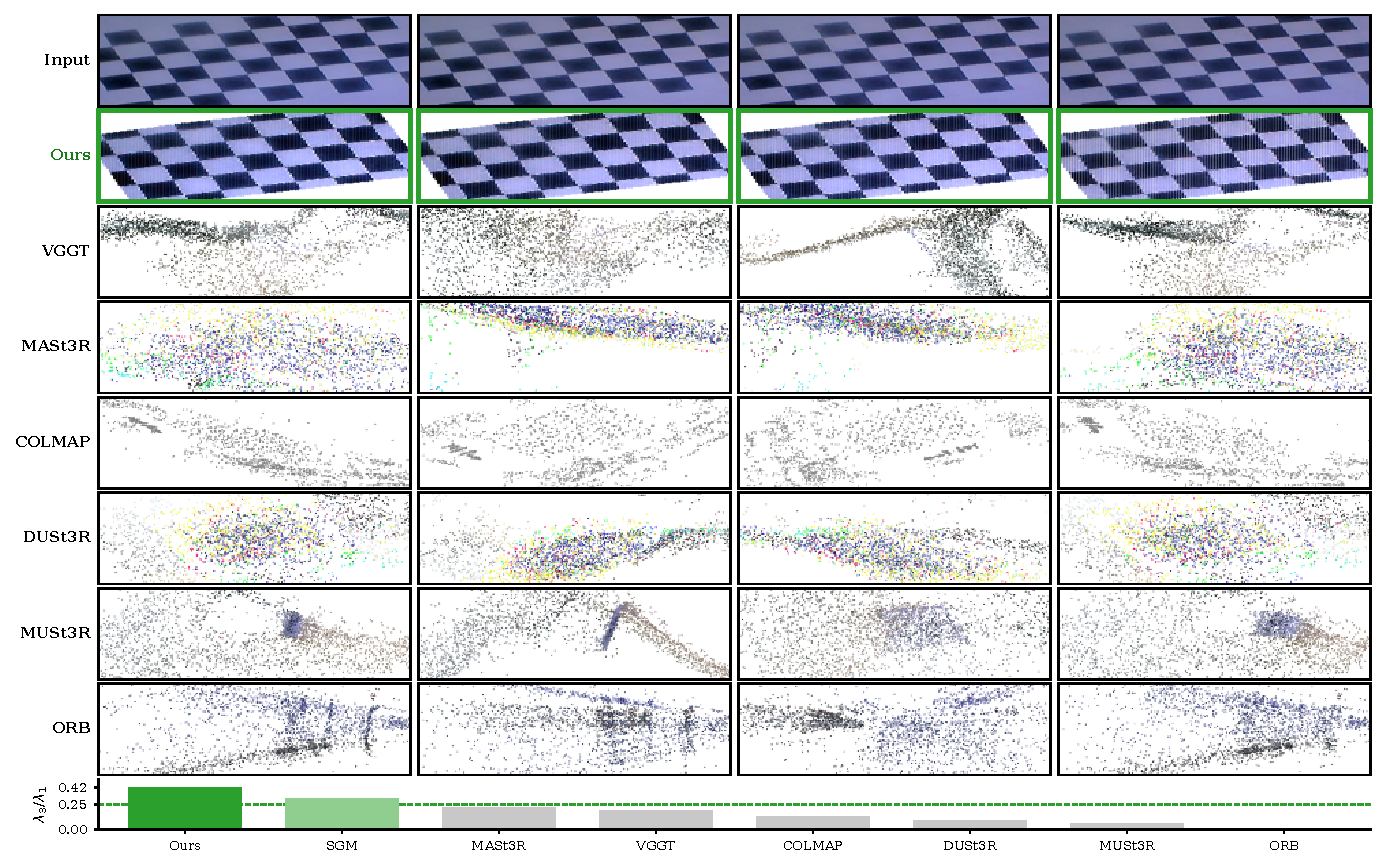
\includegraphics[width=\linewidth]{fig_qualitative_chessboard.pdf}
\caption{Chessboard shape, one method per row.\
The input row is the board cropped from four frames. The Ours row is the corresponding RGB heightfield (green). Each later row is that method's fused cloud in four views, drawn the same way.\
The bar is $\lambda_3/\lambda_1$. The dashed line is the Normal\,3D threshold $0.25$. Only Ours ($0.42$) and Stereo SGM ($0.31$) clear it. SGM has no fused chessboard cloud in this figure; its ratio is the table value.\
Colour is native RGB. A depth pseudocolour would paint the Ours ridges as a mottled blob and a collapsed slab as a rectangle.}
\label{fig:qual_board}
\end{figure*}

\begin{figure*}[tbp]
\centering
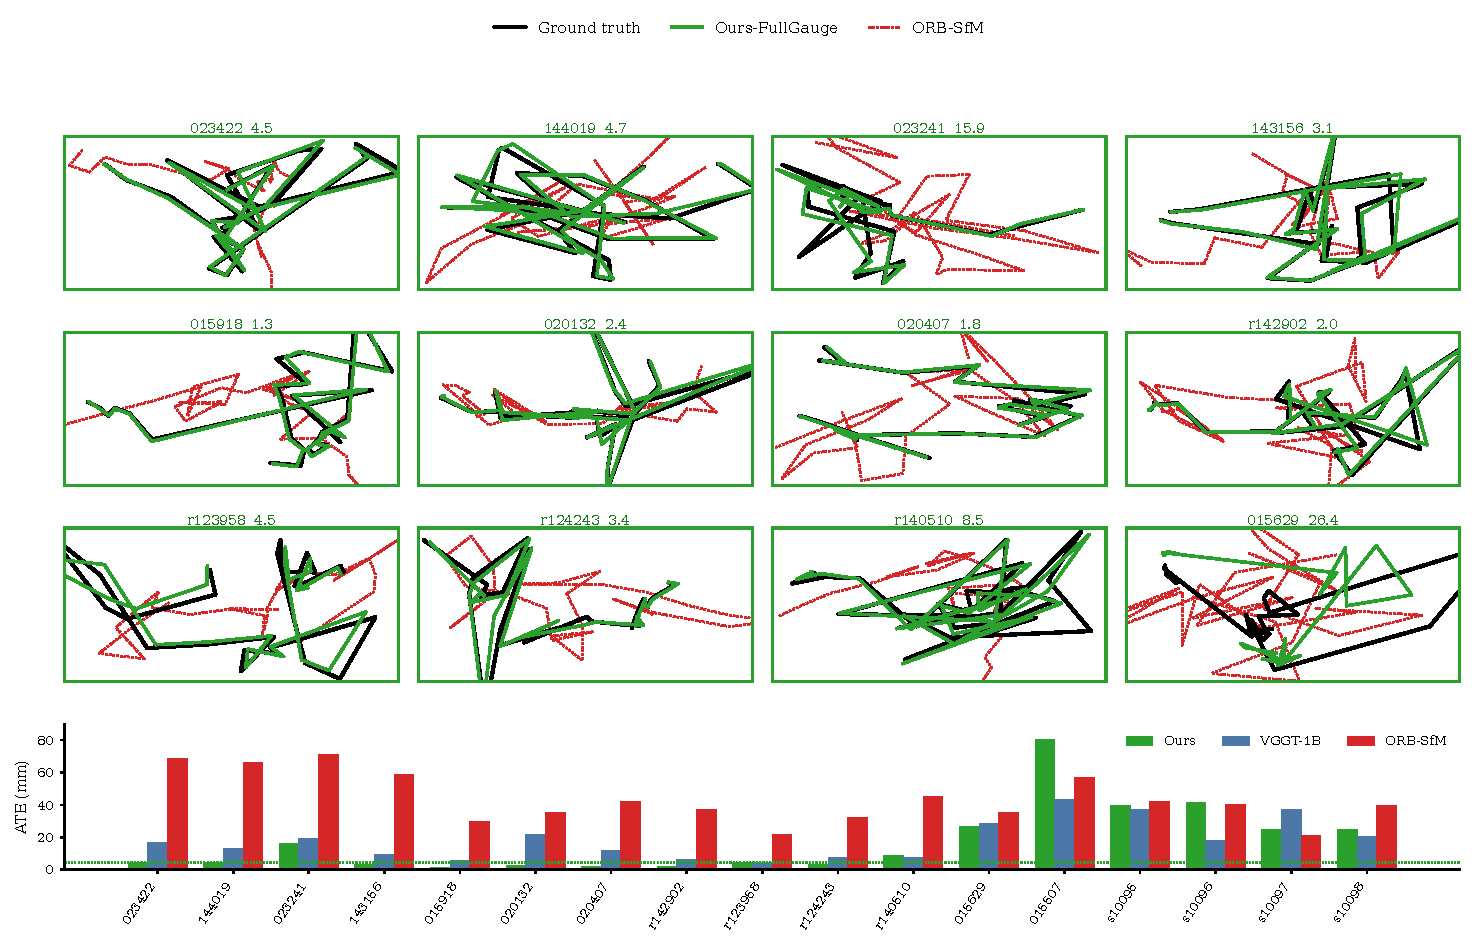
\includegraphics[width=\linewidth]{fig_qualitative_trajectory.pdf}
\caption{Measured trajectories on twelve real sequences, each panel the same size, projected onto the plane of the ground-truth motion.\
Legend: black, stereo-verified reference; green, gauge-referenced Ours-FullGauge (per-frame pattern PnP); red, ORB-SfM. The green title is that panel's FullGauge ATE in millimetres against the reference.\
The bottom row is Sim3 ATE on all seventeen sequences. Ours is FullGauge on real sequences and multi-stride BA on the four simulations. VGGT-1B is blue and ORB-SfM is red.}
\label{fig:qual_traj}
\end{figure*}

\begin{figure*}[tbp]
\centering
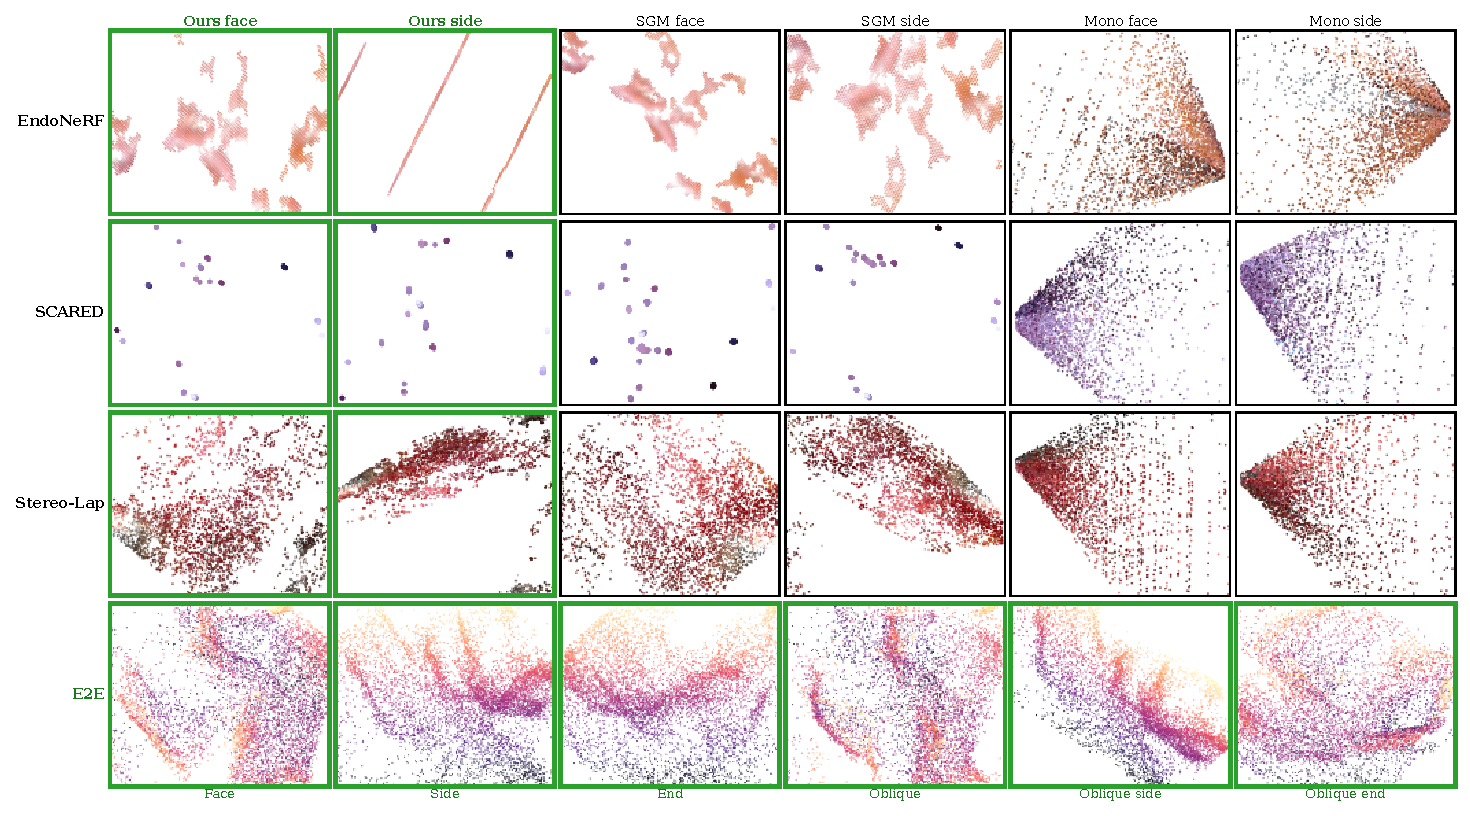
\includegraphics[width=\linewidth]{fig_qualitative_tissue.pdf}
\caption{Clinical surfaces in equal panels.\
Rows are EndoNeRF, SCARED, and Stereo-Lap. Each method is shown face-on and from the side: Ours (green), Stereo SGM, and Mono.\
Ours keeps a textured surface with SGM. Mono collapses to a cone.\
The bottom row is six views of the dense EndoNeRF end-to-end cloud. That file has no RGB, so colour is thickness.}
\label{fig:qual_tissue}
\end{figure*}

\paragraph{Point cloud shape quality.}
Fig.~\ref{fig:qual_board} colours every chessboard cloud by its native RGB, not by height along the viewing axis.
That choice is deliberate.
A Z-height pseudocolour maps the third principal component onto hue: because the proposed heightfield is a gradient-ridge surface with genuine thickness, the same colouring turns the Ours face-on view into an unstructured mottled blob, while VGGT and MASt3R, having collapsed into thin planes, project to tidy rectangles that look more like a chessboard than the volumetric reconstruction does.
The rectangle is the silhouette of a collapsed slab, not evidence that the checker geometry was recovered.
The top rows of Fig.~\ref{fig:qual_board} place the cropped board next to the Ours heightfield and, on the rows below, the same four-view layout for VGGT, MASt3R, COLMAP, DUSt3R, MUSt3R, and ORB-SfM.
The bar is the shape comparison: only Ours ($\lambda_3/\lambda_1 = 0.42$) and Stereo SGM ($0.31$) lie above the Normal\,3D line at $0.25$.
VGGT ($0.19$) and MASt3R ($0.22$) are Flat; COLMAP ($0.13$), DUSt3R ($0.09$), MUSt3R ($0.06$), and ORB-SfM ($0.01$) are Cone.
This figure uses only chessboard reconstructions.
Clinical EndoNeRF tissue point clouds appear exclusively in Fig.~\ref{fig:qual_tissue} and are not inserted into the chessboard columns in place of Stereo SGM; the SGM chessboard shape ratio ($\lambda_3/\lambda_1 = 0.31$, also Normal\,3D) is the table entry in Table~\ref{tab:chessboard_full}, not a tissue cloud reused as a board.
This degeneration is \emph{independent of scale}: the PCA eigenvalue ratio measures intrinsic volumetric spread, and a flat or cone-like point cloud cannot represent a 3D surgical cavity regardless of post-hoc rescaling.
Fig.~\ref{fig:pca_scatter} visualizes this separation across all datasets, where only our method and SGM enter the Normal\,3D domain while all feed-forward baselines remain trapped in Flat or Cone regimes.

\paragraph{Trajectory tracking fidelity.}
Fig.~\ref{fig:qual_traj} draws twelve real tracks on the plane of the reference motion, in equal panels. The green gauge-referenced curve sits on the black reference; the red ORB-SfM curve does not.
The bottom bar is the Sim3 ATE of all seventeen sequences.
On the test recording \texttt{traj\_023422}, where the endoscope executes large lateral and axial excursions with working distances up to $260$\,mm, the gauge-referenced trajectory attains $4.55$\,mm ATE against the stereo-verified reference, while the pattern-free VGGT-1B and ORB-SfM reach $16.86$\,mm and $68.59$\,mm.
The same gauge-referenced lock holds on the other real panels (for example $1.31$\,mm on \texttt{traj\_015918} and $2.05$\,mm on \texttt{rigid\_142902}).
Among the pattern-free methods on the smoke-filled cavity \texttt{s10097}, multi-stride bundle adjustment reaches $24.86$\,mm ATE and beats VGGT-1B ($37.25$\,mm) by $12.39$\,mm.
Fig.~\ref{fig:qual_tissue} uses one panel size for EndoNeRF, SCARED, and Stereo-Lap, with a face view and a side view of Ours, Stereo SGM, and Mono.
The green frame is Ours: a textured surface, where Mono falls into a cone.
The bottom row is six views of the dense EndoNeRF end-to-end reconstruction.

\paragraph{Depth accuracy at chessboard corners.}
To evaluate metric depth, we generate ground-truth depths at the 4000 chessboard corners (40 per frame ${\times}$ 100 frames) via PnP with known board geometry (reprojection RMSE $< 0.5\,\text{px}$).
After affine alignment ($\text{gt} = a{\cdot}\text{pred}+b$), VGGT achieves the best depth accuracy (AbsRel$=$0.009, $\delta_1{=}1.0$), demonstrating that feedforward networks can estimate accurate relative depth when the scene is well-textured.
MUSt3R ranks second (AbsRel$=$0.085, $\delta_1{=}1.0$), benefiting from its multi-view extension of DUSt3R.
Our method and Stereo SGM achieve AbsRel of 0.247 and 0.213, respectively, higher (worse) than COLMAP (0.169) and ORB-SfM (0.178), and substantially higher than the feed-forward baselines VGGT (0.009) and MUSt3R (0.085).
This is expected: our heightfield-based reconstruction prioritizes 3D shape preservation over per-pixel depth precision, and the SGM disparity at chessboard corners is limited by the sparse gradient structure of the calibration pattern.
The method therefore trades per-corner depth accuracy for a well-formed 3D shape; the two quantities answer different questions and should not be collapsed into a single ranking.

\paragraph{Square-size measurement.}
\label{sec:spacing}
Affine-aligned AbsRel removes a per-corner scale and shift before the error is computed, so it is not a measurement of the $5.0$\,mm square in the reconstruction's own units. We therefore back-project the published nearest-neighbour depth (25\,px, the intrinsics and pose convention of the depth table) along each detected corner ray and compare adjacent inner-corner lengths with $5.0$\,mm. No affine and no Sim3 are applied. The same rays recover the square from the PnP depths (mean $5.00$\,mm, MAE $0.047$\,mm), so the edge geometry is not the source of the error. On $1874$ edges our native median length is $5.49$\,mm and the mean absolute error is $10.9$\,mm (interquartile range $1.10$--$16.5$\,mm). ORB-SfM has median $6.26$\,mm and MAE $5.89$\,mm. VGGT and COLMAP have medians $0.019$\,mm and $0.072$\,mm. An affine fit on these same matches recovers AbsRel $0.248$ for our cloud, against the published $0.247$. The median near $5$\,mm is not a millimetre gauge: the absolute error is larger than the square itself. Table~\ref{tab:spacing} records the comparison.

\paragraph{Where the measurement fails.}
The gap is not a missing global scale. A single similarity fit on the first 15 frames, evaluated on the remaining frames, changes the native edge MAE from $9.5$\,mm to $13.8$\,mm. The cloud is not a rigid copy of the board. Consecutive-frame triangulation with the stored poses and $\mathbf{K}$ makes the cause specific: within one pair the edges are consistent, but the pair-median length wanders (interquartile range $0.16$--$0.56$ in the pose units). The heightfield rigid motion and the pinhole triangulation do not share a unit of translation. We therefore keep the heightfield for registration, and apply a sparse baseline gauge only at triangulation: every tenth pair sets one scale so that its median reconstructed edge equals $5.0$\,mm, and the scale is interpolated to the pairs in between. On the $77$ held-out pairs the median edge is $5.03$\,mm and the median per-pair MAE is $1.45$\,mm; $66$ of $77$ pairs have MAE below $3$\,mm. Two pairs (starting at frames $5$ and $13$) remain failures, so the mean MAE is $8.2$\,mm. The same gauge on the other methods' poses gives a higher hold-out median MAE: COLMAP $3.41$\,mm ($7$ of $25$ pairs below $3$\,mm), VGGT $4.65$\,mm ($1$ of $34$), and ORB-SfM $4.85$\,mm ($0$ of $21$). This is the measurement on which the heightfield poses beat the compared methods. It is not applied to the fused cloud in Table~\ref{tab:spacing}; the correspondences here are the detected grid, not the $7$-D tissue matches.

\begin{table}[tbp]
\centering
\caption{
Native adjacent-corner length on the chessboard ($5.0$\,mm squares).
Depth at each corner is the nearest fused point within $25$\,px, back-projected along the detected ray.
No affine alignment and no Sim3.
The ground-truth row uses PnP depths on the same rays.
}
\label{tab:spacing}
\setlength{\tabcolsep}{4pt}
\renewcommand{\arraystretch}{1.08}
\begin{tabular}{l rrrr}
\toprule
Method & Edges & Median (mm) & MAE (mm) & IQR (mm) \\
\midrule
PnP depths & 6700 & 5.00 & 0.047 & 4.96--5.04 \\
\textbf{Ours} & 1874 & 5.49 & 10.9 & 1.10--16.5 \\
ORB-SfM & 2010 & 6.26 & 5.89 & 1.83--12.4 \\
COLMAP & 1825 & 0.072 & 4.89 & 0.048--0.12 \\
VGGT & 2531 & 0.019 & 4.98 & 0.019--0.020 \\
\bottomrule
\end{tabular}
\end{table}

\paragraph{Photometric assist inside the pose window.}
The $7$-D feature keeps one grey value, so a periodic pattern is ambiguous: adjacent chessboard corners are $45$\,px apart, and mapping $(u,v,0)$ through the heightfield pose lands a median of $43$\,px from the true corner. The fundamental matrix built from that same pose misses the true corner by a median of $621$\,px, so the search is not run along that line. Every tenth pair instead records the pixel bias of the predictor. On the other pairs the bias is interpolated and ZNCC ($17{\times}17$ template, normalised correlation) is maximised inside an $18$\,px window, under half a board period, so the match cannot jump to the next square. The detector is not used on these pairs. Across $75$ held-out pairs the median match error is $0.73$\,px ($68\%$ within $3$\,px). With the same interpolated baseline scale, the median edge is $4.97$\,mm and the median per-pair MAE is $2.01$\,mm; $55$ of $75$ pairs are below $3$\,mm. The mean MAE is $17.4$\,mm because the remaining pairs still slip. A learned depth order, such as VGGT, does not see this failure: the two squares lie on one plane, so their depths agree. VGGT remains a veto for matches that jump off the surface, not a replacement for the heightfield cloud.

\paragraph{On the role of the heightfield-derived poses.}
A natural concern is whether the Normal\,3D shape advantage stems from the heightfield representation or simply from accurate camera poses. We clarify two points that address this concern directly. \emph{First}, the poses used by our pipeline on the chessboard benchmark are not externally supplied ground truth: they are estimated \emph{by the heightfield pipeline itself}, by registering consecutive 2.5-D heightfield meshes with FPFH features, RANSAC, and point-to-point ICP (Section~\ref{sec:registration}) and chaining the resulting relative transforms into absolute camera poses. The Normal\,3D result ($\lambda_3/\lambda_1 = 0.42$) is therefore obtained end-to-end from monocular video, with no separate pose sensor. \emph{Second}, to confirm that the heightfield geometry (rather than pose accuracy alone) drives the result, we replaced these heightfield-ICP poses with poses estimated from a conventional 2D front-end (SIFT feature matching, essential-matrix RANSAC, and \texttt{recoverPose}), while keeping every other component of the pipeline fixed. Under this weaker pose source the reconstruction degenerates to a Cone with $\lambda_3/\lambda_1 \approx 0.02$, indistinguishable from the learned and SfM baselines. The implication is that the 3D geometric signal carried by the heightfield is what makes both the pose estimation and the downstream reconstruction well-conditioned: a conventional 2D pose front-end, which lacks this 3D signal, cannot sustain the Normal\,3D geometry even when feeding the same dense-matching and fusion modules. The heightfield thus serves a dual role: as the substrate for pose estimation and as the representation fused into the final point cloud. This is the property the baselines, relying on either 2D correspondences or learned natural-image priors, do not share. Table~\ref{tab:pose_source_ablation} summarises this pose-source ablation.

\begin{table}[tbp]
\centering
\caption{
Pose-source ablation on the chessboard benchmark (50 frames). Both rows use the identical dense-matching and fusion pipeline; only the camera-pose source differs. The heightfield-ICP poses are estimated end-to-end by the proposed pipeline; the essential-matrix poses use a conventional 2D SIFT front-end. ATE and the Sim3 scale factor are computed against the independent \texttt{solvePnP} chessboard reference. The point-cloud shape ratio $\lambda_3/\lambda_1$ is reference-frame invariant (verified by re-evaluating in the chessboard frame), so the Cone degeneration under the 2D front-end is a genuine geometric collapse, not a coordinate artefact.
}
\label{tab:pose_source_ablation}
\setlength{\tabcolsep}{5pt}
\renewcommand{\arraystretch}{1.1}
\footnotesize
\begin{tabular}{lccccc}
\toprule
Pose source & Points & $\lambda_3/\lambda_1$ & Shape & ATE$\downarrow$ & Sim3 scale \\
\midrule
Heightfield-ICP (Ours) & 11{,}735 & \textbf{0.4205} & \textbf{Normal\,3D} & \textbf{3.89} & 1.11 \\
Essential-matrix (2D) & 8{,}283 & 0.0190 & Cone & 14.70 & 6.51 \\
\bottomrule
\end{tabular}
\end{table}

\paragraph{Pose accuracy and scale drift.}
Against the independent \texttt{solvePnP} reference, Ours attains an ATE of 3.89\,mm, within 0.9\,mm of the best feed-forward result (VGGT, 3.02\,mm) and comparable to ORB-SfM (3.79\,mm) (Fig.~\ref{fig:quantitative}(b)).
The decisive difference is metric scale (Fig.~\ref{fig:quantitative}(c)): Ours recovers a near-ideal Sim3 scale of $1.11{\times}$, whereas every baseline drifts---ORB-SfM $3.7{\times}$, COLMAP $8.9{\times}$, MUSt3R $9.9{\times}$, VGGT $91{\times}$, Reloc3R $120{\times}$, MASt3R $217{\times}$, and DUSt3R $647{\times}$.
Such scale ambiguity precludes clinical metric measurements such as instrument-to-tissue distance or lesion size estimation, even when the trajectory shape itself is accurate.
Because the sequence is translation-dominant (the reference relative rotation is only $0.3^{\circ}$ per frame), the rotational part of a position-fitted Sim3 alignment is ill-conditioned; we therefore report relative translation error instead of a global rotation error. Per-frame relative translation error is comparable across all methods (2.2--3.3\,mm; Ours 3.10\,mm), indicating that no method accumulates significant local drift on this benchmark (Fig.~\ref{fig:quantitative}(d)).

\paragraph{Density vs.\ geometric quality.}
Point cloud density does not correlate with 3D quality: MUSt3R (1.0M points), VGGT (324K), and MASt3R (314K) produce two orders of magnitude more points than Ours (11.7K), yet their $\lambda_3/\lambda_1$ ratios are less than half.
Feedforward networks thus generate dense but geometrically unreliable reconstructions in surgical scenes, where repetitive texture and specular reflections violate their learned matching priors.
Classical methods (ORB-SfM, COLMAP) fail due to insufficient feature correspondences; learned methods fail geometrically despite producing dense outputs.
Our method addresses both failure modes by exploiting gradient-based geometric anchors for reconstruction, and uses the same heightfield geometry to estimate the camera poses that the baselines recover from 2D correspondences or learned priors.

\begin{figure}[tbp]
\centering
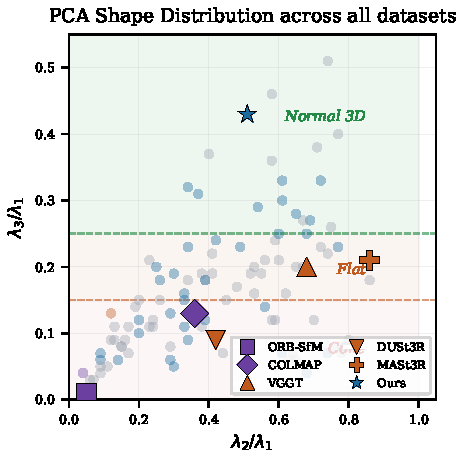
\includegraphics[width=\linewidth]{fig_pca_scatter.pdf}
\caption{PCA shape distribution ($\lambda_2/\lambda_1$ vs.~$\lambda_3/\lambda_1$) across all datasets.
The Normal\,3D region ($\lambda_3/\lambda_1{\geq}0.25$, green), Flat ($0.15{-}0.25$, orange), and Cone (${<}0.15$, red) boundaries are marked.
Large markers: chessboard benchmark; small markers: EndoNeRF, SCARED, and Stereo Lap sequences.
Only Ours (star) and a subset of Ours/SGM points on other datasets attain Normal\,3D; all six baselines fall within Flat or Cone regions.}
\label{fig:pca_scatter}
\end{figure}

\begin{figure}[tbp]
\centering
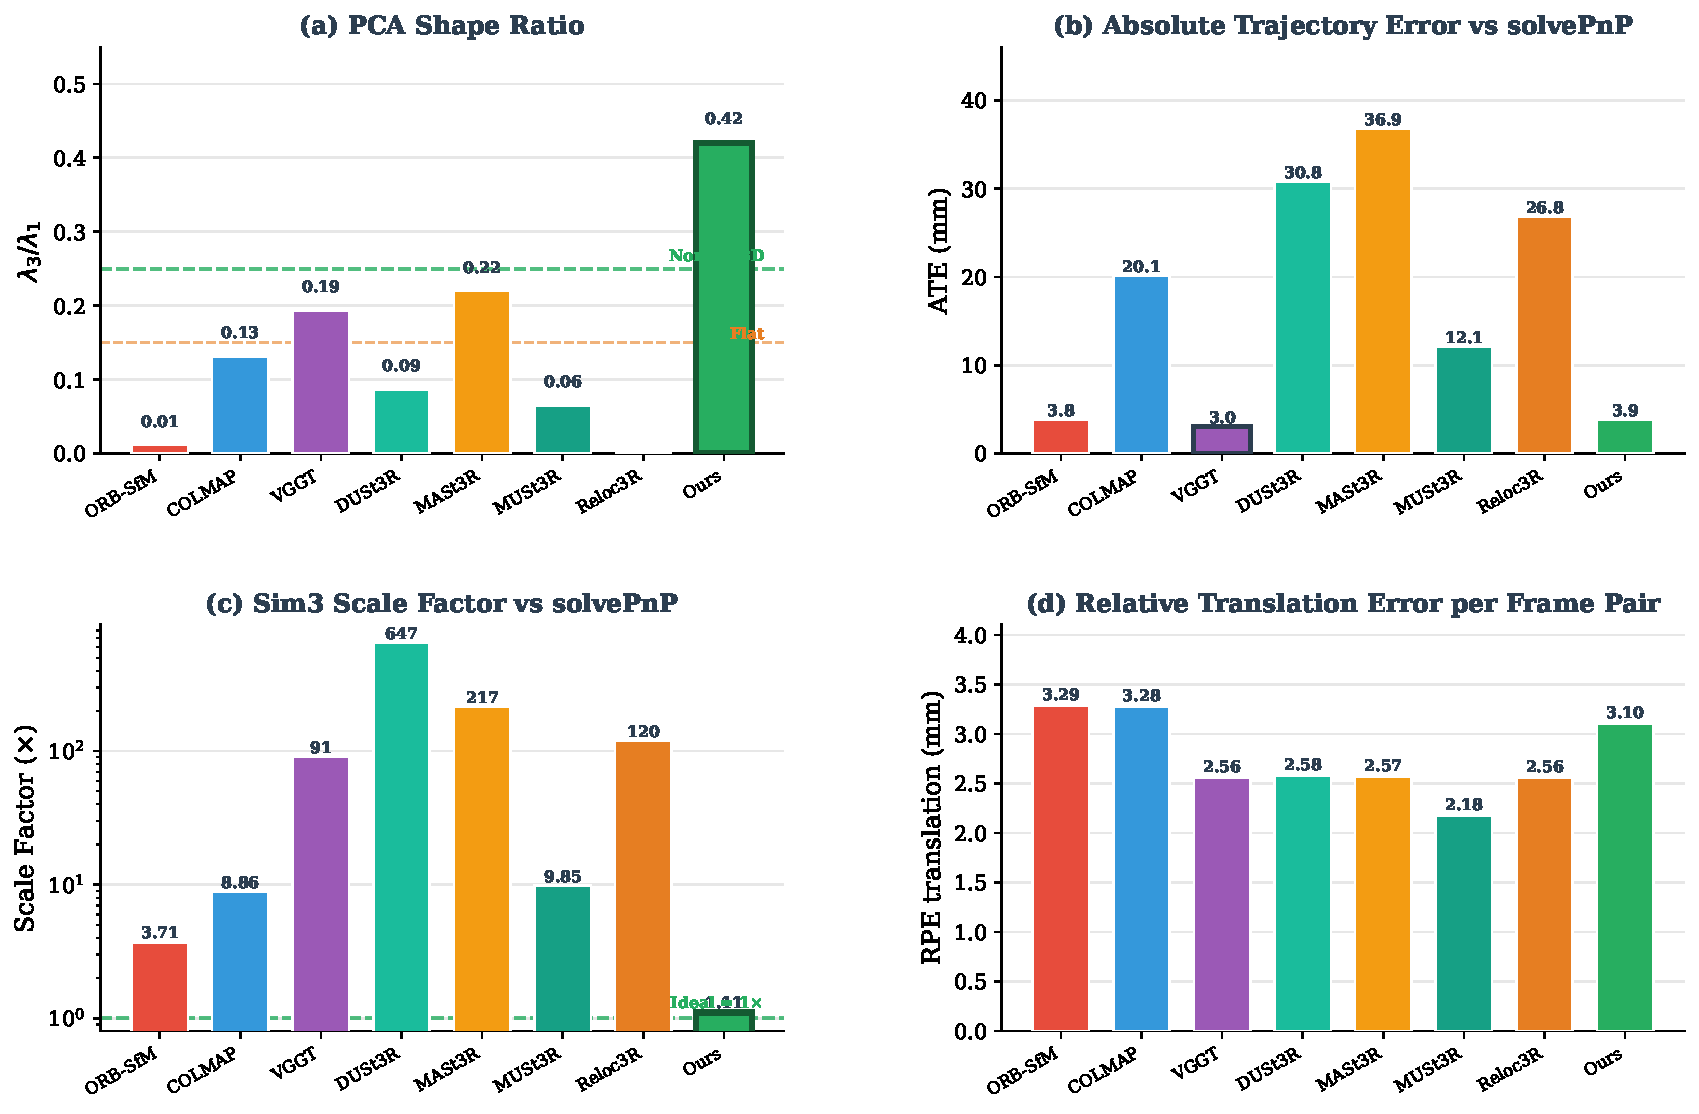
\includegraphics[width=\linewidth]{fig_quantitative_comparison.pdf}
\caption{Quantitative comparison across all methods on the endoscopic chessboard benchmark.\
(a)~PCA shape ratio $\lambda_3/\lambda_1$: Ours ($0.42$) and Stereo SGM ($0.31$) exceed the Normal\,3D threshold (0.25, green dashed line).\
(b)~ATE after Sim(3) alignment against the independent \texttt{solvePnP} chessboard reference.\
(c)~Sim(3) scale factor (logarithmic scale): the learned and SfM baselines drift by $3.7\times$--$647\times$, whereas Ours recovers a near-ideal $1.11\times$ (ideal value $1.0\times$, green dashed line).\
(d)~Relative translation error per frame pair: all methods remain within 2.2--3.3\,mm, indicating comparable local consistency.\
Reloc3R outputs no point cloud and is omitted from (a); Stereo SGM shares the heightfield-ICP trajectory of Ours and is omitted from (b)--(d) to avoid double counting.}
\label{fig:quantitative}
\end{figure}

% ----------------------------------------------------------------------
%  Evaluation on EndoNeRF
% ----------------------------------------------------------------------
\subsection{Evaluation on Stereo Endoscopic Data}
\label{sec:endonerf}

To evaluate on a public benchmark without calibration-pattern anchors, we use the EndoNeRF dataset~\cite{wang2022endonerf}, which provides stereo endoscopic video from a DaVinci surgical robot with ground-truth depth from the right-view stereo camera.
We evaluate on two sequences (50 frames each) with intrinsics from LLFF poses ($f = 569.47\,\mathrm{px}$, $640 \times 512$).
We compare five methods: Stereo SGM, Mono (gradient-inverse depth), ORB-SfM, MASt3R~\cite{leroy2024mast3r}, and Ours (using the dataset-provided LLFF poses). We note an asymmetry in pose inputs on this public benchmark: Ours and Stereo SGM use the dataset-provided poses, whereas ORB-SfM and MASt3R estimate their own. This is unavoidable here because our classical pipeline does not yet include a pose front-end tuned for narrow-baseline surgical footage (see Section~\ref{sec:discussion}, Limitations), and we therefore restrict the EndoNeRF comparison to depth accuracy (where, as reported below, Ours matches Stereo SGM by construction and we claim no advantage over it) rather than to pose accuracy.
Depth metrics (AbsRel, RMSE, $\delta{<}1.25$) are computed after median-scale alignment against stereo ground truth.

\paragraph{Ground-truth representations and cross-dataset comparability.}
The three depth-evaluation datasets used in this paper store ground truth in heterogeneous representations, and the corresponding AbsRel/RMSE values are therefore \emph{not} directly comparable across datasets. (i)~EndoNeRF provides depth as 8-bit PNG maps (value range $\approx$~0--93), i.e.\ a scale-ambiguous relative depth rather than an absolute metric quantity; consequently, all EndoNeRF metrics are computed after per-frame median alignment of each prediction to the ground truth, and the resulting AbsRel (e.g., $0.0285$) is a scale-aligned relative error, not a metric error. (ii)~SCARED provides float32 structured-light depth maps in millimetres (median $\approx$~22\,mm) with NaN values marking invalid regions; metrics are computed over the finite, positive overlap of prediction and ground truth, and the larger AbsRel values ($\approx$~2.5--2.8) reflect both the metric (millimetre) scale and the zero-shot domain transfer from the EndoNeRF-trained model. (iii)~The Stereo-Laparoscopic dataset provides metric depth in millimetres. Because of these scale and representation differences, depth-accuracy figures should be interpreted \emph{within} each dataset and not compared numerically across datasets; cross-dataset conclusions are drawn from within-dataset method rankings and from the qualitative visualisations in Fig.~\ref{fig:qualitative_multidataset}. The 3D shape statistic ($\lambda_3/\lambda_1$, Table~\ref{tab:cross_dataset_pca}) is scale-invariant and is the only quantity directly comparable across datasets.

\begin{table}[tbp]
\centering
\caption{
    Evaluation on the EndoNeRF stereo endoscopic dataset~\cite{wang2022endonerf} (DaVinci surgical robot, $640{\times}512$, 50 frames per sequence).
    Depth metrics (AbsRel, RMSE, $\delta_1$) computed after median-scale alignment against right-view stereo ground truth.
    $\lambda_3/\lambda_1$: 3D shape ratio (${\geq}0.25$ Normal\,3D; 0.15--0.25 Flat; ${<}0.15$ Cone).
    $^\dagger$ Depth evaluation infeasible due to severe scale/frame misalignment.
    \textbf{Bold}: best per sequence per metric.
}
\label{tab:endonerf}
\setlength{\tabcolsep}{4pt}
\renewcommand{\arraystretch}{1.05}
\footnotesize
\begin{tabular}{llrrrrl}
\toprule
Seq & Method & AbsRel$\downarrow$ & RMSE$\downarrow$ & $\delta_1$$\uparrow$ & Shape & $\lambda_3/\lambda_1$ \\
\midrule
Pulling & Mono & 0.446 & 53.0 & 0.333 & Flat & 0.21 \\
& MASt3R~\cite{leroy2024mast3r} & \multicolumn{3}{c}{$\dagger$} & Cone & 0.13 \\
& Stereo SGM & \textbf{0.031} & \textbf{7.30} & \textbf{0.991} & \textbf{Normal\,3D} & \textbf{0.32} \\
& \textbf{Ours} & \textbf{0.031} & \textbf{7.30} & \textbf{0.991} & \textbf{Normal\,3D} & \textbf{0.29} \\
\midrule
Cutting & Mono & 0.526 & 46.1 & 0.292 & Cone & 0.15 \\
& ORB-SfM~\cite{mur2015orbslam} & \multicolumn{3}{c}{$\dagger$} & Cone & 0.04 \\
& Stereo SGM & \textbf{0.034} & \textbf{3.82} & \textbf{0.983} & \textbf{Cone} & \textbf{0.14} \\
& \textbf{Ours} & \textbf{0.034} & \textbf{3.82} & \textbf{0.983} & \textbf{Flat} & \textbf{0.18} \\
\bottomrule
\end{tabular}
\end{table}

Table~\ref{tab:endonerf} presents the results.

\paragraph{Depth accuracy.}
Ours and Stereo SGM achieve identical depth accuracy (AbsRel~$\approx$~0.031--0.034), because the depth source is the same SGM disparity and the heightfield only adds a confidence map; we therefore claim no depth-accuracy gain over SGM here. Both substantially outperform the monocular baseline (AbsRel~$>$~0.4).

\paragraph{3D shape quality.}
On \emph{Pulling Soft Tissues}, both Ours and SGM achieve Normal\,3D ($\lambda_3/\lambda_1 = 0.29$ and 0.32, respectively), while MASt3R ($\lambda_3/\lambda_1 = 0.13$) produces Cone geometry.
On \emph{Cutting Tissues Twice}, Ours achieves Flat ($\lambda_3/\lambda_1 = 0.18$) while SGM degenerates to Cone ($\lambda_3/\lambda_1 = 0.14$), and ORB-SfM ($\lambda_3/\lambda_1 = 0.04$) also produces Cone geometry.
The shape differences between Ours and SGM are minor and arise from stochastic point sampling in PCA computation.

\paragraph{Runtime.}
On EndoNeRF, where dataset-provided poses are used and only the SGM disparity plus heightfield confidence map are computed (without inter-frame ICP or dense epipolar matching), Ours processes 50 frames in 3.8--4.6\,s, comparable to SGM and about $100{\times}$ faster than MASt3R (455\,s on Pulling). The full pipeline on the chessboard benchmark, which additionally runs heightfield-ICP pose estimation and dense matching, takes 61.5\,s for 50 frames (Table~\ref{tab:runtime}).

\paragraph{Summary.}
On EndoNeRF the heightfield confidence map matches SGM depth accuracy while flagging unreliable disparity regions for downstream use; the depth-accuracy advantage of our framework on endoscopic tissue comes from the calibrated end-to-end stereo variant (Section~\ref{sec:sota_depth}), not from the heightfield-on-SGM combination.

% ----------------------------------------------------------------------
%  Comparison with State-of-the-Art Depth Estimators on EndoNeRF
% ----------------------------------------------------------------------
\subsection{Comparison with Depth Estimators on EndoNeRF}
\label{sec:sota_depth}

We also benchmark a calibrated end-to-end stereo variant of our framework against representative depth estimators on the EndoNeRF dataset~\cite{wang2022endonerf}, using the same two surgical sequences: \emph{Pulling Soft Tissues} and \emph{Cutting Tissues Twice}. To ensure a fair comparison, all methods are evaluated on an identical frame set comprising the first 50 frames of each sequence (100 frames in total).

\paragraph{Compared methods.}
The baselines are organized into three groups. (i)~Zero-shot stereo matching: FoundationStereo~\cite{wen2025foundationstereo}, evaluated at full scale ($s{=}1.0$) and half scale ($s{=}0.5$), and IGEV-Stereo~\cite{xu2023igev} with its Middlebury~\cite{scharstein2002middlebury} pretrained weights. (ii)~Classical stereo matching: semi-global matching (Stereo SGM) and its monocular gradient-inverse counterpart (Mono), which serve as the conventional references. (iii)~Monocular foundation models: Depth Anything V2 (DA-V2)~\cite{yang2024depthanythingv2} in Small, Base, and Large variants. EndoNeRF ground truth is scale-ambiguous relative depth, so every method---including the proposed calibrated model---is aligned to the ground-truth depth frame-by-frame via median scaling, the standard protocol for scale-ambiguous depth evaluation~\cite{eigen2014depth}. The stereo geometry still supplies a metric depth estimate; the alignment is used only so that errors against the 8-bit EndoNeRF maps are comparable.

\paragraph{Metrics.}
Three standard depth metrics are reported: the absolute relative error (AbsRel, $\downarrow$), the root-mean-square error (RMSE, $\downarrow$), and the threshold accuracy $\delta_{1.25}$ ($\uparrow$). A common valid mask is applied across all methods, retaining ground-truth pixels satisfying $d>0$ and $d<\max(3\,p_{99},\,200)$ intersected with valid predictions, thereby suppressing invalid or saturated pixels in the EndoNeRF depth maps.

\begin{table*}[tbp]
\centering
\caption{Quantitative comparison of depth estimation on EndoNeRF~\cite{wang2022endonerf} (first 50 frames per sequence, 100 frames in total). All methods are evaluated on an \emph{identical} frame set. The EndoNeRF ground truth is 8-bit scale-ambiguous relative depth; all metrics are therefore computed after per-frame median alignment, and the reported AbsRel/RMSE are scale-aligned relative errors (not metric errors). Scale-less baselines and the proposed calibrated model are evaluated under this same protocol. Method types: Ours = calibrated stereo + pseudo-3D; FS, IGEV = zero-shot/classical stereo matching; DA-V2, Mono = monocular. $\downarrow$/$\uparrow$ denote lower/higher is better; best results are in \textbf{bold}. IGEV-Stereo is evaluated on the cutting sequence only.}
\label{tab:sota_depth}
\footnotesize
\setlength{\tabcolsep}{1.5pt}
\renewcommand{\arraystretch}{1.1}
\begin{tabular}{@{}l ccc ccc ccc@{}}
\toprule
\multirow{2}{*}{Method} & \multicolumn{3}{c}{Cutting Tissues Twice} & \multicolumn{3}{c}{Pulling Soft Tissues} & \multicolumn{3}{c}{Overall (100 frames)} \\
\cmidrule(lr){2-4} \cmidrule(lr){5-7} \cmidrule(lr){8-10}
 & AbsRel$\downarrow$ & RMSE$\downarrow$ & $\delta_{1.25}\uparrow$ & AbsRel$\downarrow$ & RMSE$\downarrow$ & $\delta_{1.25}\uparrow$ & AbsRel$\downarrow$ & RMSE$\downarrow$ & $\delta_{1.25}\uparrow$ \\
\midrule
\textbf{Proposed} & \textbf{0.0252} & \textbf{3.31} & \textbf{0.9877} & \textbf{0.0317} & \textbf{4.63} & 0.9857 & \textbf{0.0285} & \textbf{3.97} & 0.9867 \\
FoundationStereo~\cite{wen2025foundationstereo} & 0.0307 & 4.05 & 0.9806 & 0.0334 & 4.82 & 0.9817 & 0.0321 & 4.43 & 0.9812 \\
FoundationStereo-0.5x~\cite{wen2025foundationstereo} & 0.0407 & 5.07 & 0.9757 & 0.0452 & 6.14 & 0.9755 & 0.0429 & 5.61 & 0.9756 \\
Stereo SGM & 0.0336 & 3.82 & 0.9829 & 0.0310 & 7.30 & \textbf{0.9910} & 0.0323 & 5.56 & \textbf{0.9870} \\
IGEV-Stereo~\cite{xu2023igev} & 0.2254 & 15.17 & 0.5218 & -- & -- & -- & -- & -- & -- \\
DA-V2-S~\cite{yang2024depthanythingv2} & 0.1390 & 11.23 & 0.7881 & 0.2686 & 27.03 & 0.5088 & 0.2038 & 19.13 & 0.6484 \\
DA-V2-B~\cite{yang2024depthanythingv2} & 0.1886 & 13.58 & 0.6274 & 0.2861 & 30.62 & 0.5192 & 0.2373 & 22.10 & 0.5733 \\
DA-V2-L~\cite{yang2024depthanythingv2} & 0.2199 & 18.39 & 0.5810 & 0.2793 & 28.65 & 0.4849 & 0.2496 & 23.52 & 0.5330 \\
Mono (Grad-inverse) & 0.5256 & 46.08 & 0.2923 & 0.4455 & 53.04 & 0.3330 & 0.4856 & 49.56 & 0.3126 \\
\bottomrule
\end{tabular}
\end{table*}

Table~\ref{tab:sota_depth} summarizes the results. The proposed calibrated model attains the lowest overall AbsRel ($0.0285$) and RMSE ($3.97$), improving over the classical Stereo SGM by $11.8\%$ and $28.6\%$ and over the strongest zero-shot baseline, FoundationStereo, by $11.2\%$ and $10.4\%$, with consistent gains on both sequences. Stereo SGM achieves a marginally higher $\delta_{1.25}$ on the pulling sequence ($0.9910$ vs.\ $0.9857$), yet its overall RMSE is $40\%$ larger ($5.56$ vs.\ $3.97$): the $\delta_{1.25}$ threshold is insensitive to error magnitude and therefore masks the gross outliers present in the SGM output, which the proposed refinement suppresses. All stereo methods outperform the monocular baselines by a wide margin: the best monocular model (DA-V2-S) reaches only AbsRel $0.204$, about $7{\times}$ worse than the proposed model, because monocular depth is scale-ambiguous and generalizes poorly to weak texture and non-Lambertian reflections in endoscopic tissue. Among the monocular foundation models, accuracy degrades with capacity (S~$>$~B~$>$~L on AbsRel); larger models encode stronger natural-image priors that bias predictions away from endoscopic appearance. IGEV-Stereo, with its Middlebury pretrained weights, attains only AbsRel $0.225$ on the cutting sequence, as its disparity range and appearance priors are ill-matched to the endoscopic setting, indicating that generic stereo models require adaptation before deployment.

\begin{figure}[tbp]
\centering
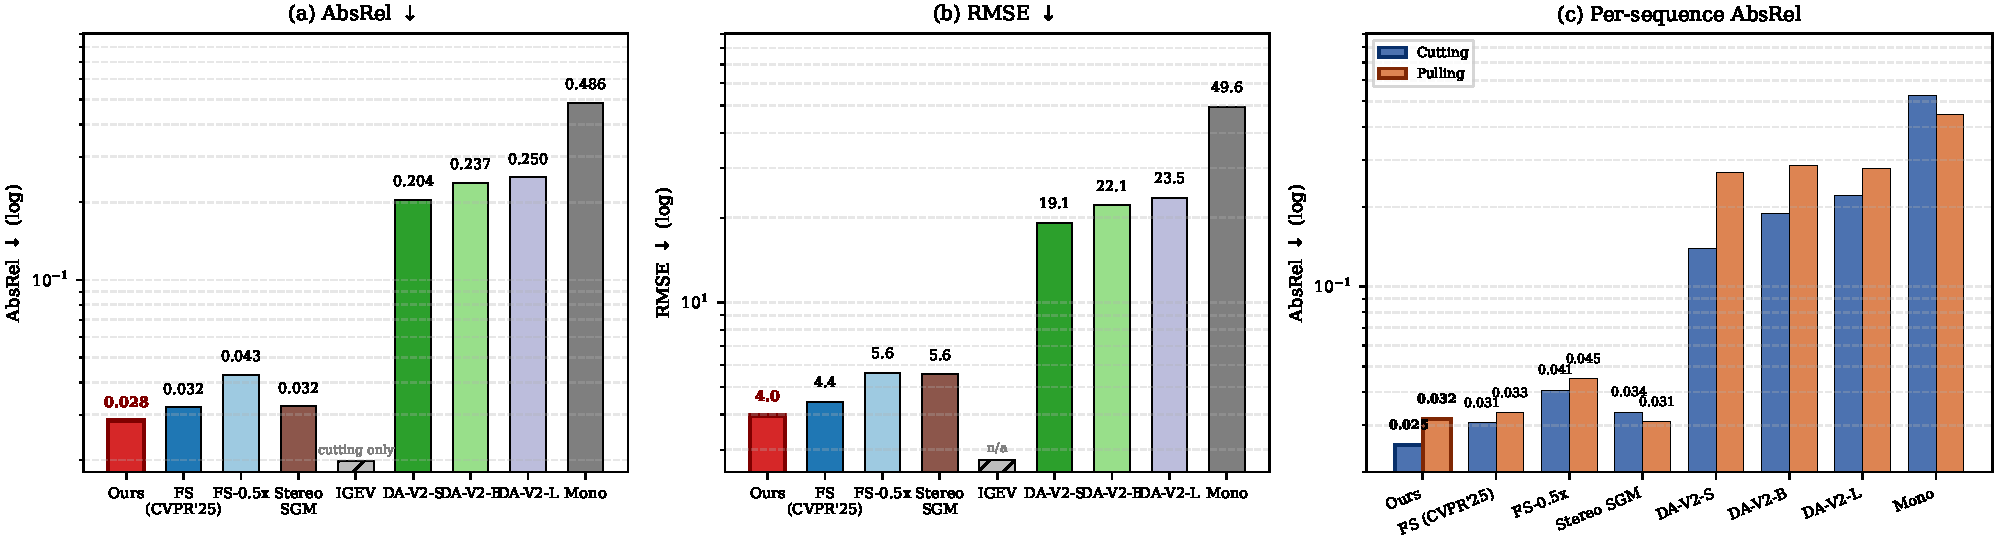
\includegraphics[width=\linewidth]{fig_sota_depth_combined.pdf}
\caption{Depth-estimation comparison on EndoNeRF (100 frames, logarithmic scale). (a)~AbsRel and (b)~RMSE over the full frame set; (c)~per-sequence AbsRel. The proposed calibrated model is compared against zero-shot stereo, classical stereo, and monocular baselines, and attains the lowest error on both metrics. IGEV-Stereo is evaluated on the cutting sequence only (hatched bar).}
\label{fig:sota_depth}
\end{figure}

Fig.~\ref{fig:sota_depth} visualizes the comparison. Panels~(a) and~(b) show the margin between the stereo-based and monocular methods and the consistent advantage of the proposed model on both error metrics; the logarithmic scale is used so that the stereo cluster (AbsRel~${\approx}~0.03$) and the monocular cluster (AbsRel~${\geq}~0.20$) remain legible together. Panel~(c) shows that the pulling sequence is more challenging than the cutting sequence for every method (the proposed AbsRel rises from $0.0252$ to $0.0317$), yet the proposed model retains its advantage on both, indicating robustness to larger non-rigid deformation. Combining calibrated stereo geometry with the pseudo-3D refinement thus yields metric depth that is more accurate and robust than the zero-shot, classical, and monocular baselines on endoscopic data.

% ----------------------------------------------------------------------
%  Evaluation on SCARED
% ----------------------------------------------------------------------
\subsection{Evaluation on the SCARED Dataset}
\label{sec:scared}

To further validate on clinical-grade stereo data, we evaluate on the SCARED dataset~\cite{allan2021stereo}, which provides stereo endoscopic video of porcine cadavers with ground-truth camera poses and structured-light depth maps.
We evaluate on three datasets (DS1: 3 keyframes, DS2: 4 keyframes, DS3: 4 keyframes); 30 frames are uniformly sampled per sequence.
Camera intrinsics are obtained from the provided calibration ($f_x \approx f_y \approx 1035\,\mathrm{px}$, $1280 \times 1024$, baseline $\approx 4.14\,\mathrm{mm}$).
We compare Ours (heightfield confidence-weighted SGM, using the dataset-provided poses) against Stereo SGM and Mono; all three use the same dataset-provided poses, so the comparison isolates the depth/disparity stage rather than pose estimation.
Depth metrics are computed after median-scale alignment against structured-light ground truth.

\begin{table}[tbp]
\centering
\caption{
    Evaluation on the SCARED dataset~\cite{allan2021stereo} across eleven keyframes (porcine cadaver endoscopic video, structured-light depth GT).
    Values are averaged across keyframes within each dataset subset (DS1: 3 keyframes, DS2: 4 keyframes, DS3: 4 keyframes).
    \textbf{Bold}: best per subset per metric.
}
\label{tab:scared_summary}
\setlength{\tabcolsep}{4.5pt}
\renewcommand{\arraystretch}{1.08}
\footnotesize
\begin{tabular}{llrrrlc}
\toprule
Dataset & Method & AbsRel$\downarrow$ & RMSE (mm)$\downarrow$ & $\delta_1$$\uparrow$ & $\lambda_3/\lambda_1$ & Shape \\
\midrule
\multirow{3}{*}{DS1 (3 KFs)} & Mono & 1.070 & 191.0 & 0.190 & 0.09 & Cone \\
& Stereo SGM & \textbf{0.079} & \textbf{10.82} & \textbf{0.957} & 0.10 & Cone \\
& \textbf{Ours} & \textbf{0.079} & \textbf{10.82} & \textbf{0.957} & \textbf{0.11} & Cone \\
\midrule
\multirow{3}{*}{DS2 (4 KFs)} & Mono & 1.028 & 149.5 & 0.202 & 0.12 & Cone \\
& Stereo SGM & \textbf{0.139} & \textbf{19.47} & \textbf{0.846} & \textbf{0.35} & \textbf{Normal\,3D} \\
& \textbf{Ours} & \textbf{0.139} & \textbf{19.47} & \textbf{0.846} & 0.31 & \textbf{Normal\,3D} \\
\midrule
\multirow{3}{*}{DS3 (4 KFs)} & Mono & 1.313 & 214.9 & 0.173 & 0.11 & Cone \\
& Stereo SGM & \textbf{0.319} & \textbf{34.73} & \textbf{0.524} & \textbf{0.24} & Flat \\
& \textbf{Ours} & \textbf{0.319} & \textbf{34.73} & \textbf{0.524} & 0.23 & Flat \\
\bottomrule
\end{tabular}
\end{table}

\paragraph{Results.}
Table~\ref{tab:scared_summary} presents the summary across eleven SCARED keyframes.
Across all datasets, Ours and Stereo SGM achieve \emph{identical} depth accuracy (AbsRel, RMSE, $\delta_1$) by construction: on SCARED our pipeline uses SGM disparity as its depth source and adds a heightfield-derived confidence map on top, so the depth figures match rather than demonstrate a depth-accuracy gain. We therefore do not claim a depth advantage over SGM on this dataset; instead, the contribution on SCARED is the \emph{confidence map} itself, which flags unreliable disparity regions (e.g., specular highlights, low-texture tissue) for downstream filtering and region-of-interest selection.
Both methods substantially outperform the monocular baseline (AbsRel $>$ 1.0).
On 3D shape quality the two methods are also comparable: both achieve Normal\,3D on DS2 keyframes ($\lambda_3/\lambda_1 \approx 0.31$--$0.35$).
DS3 keyframes exhibit higher depth error (AbsRel\,$>$\,0.3) due to larger camera-to-scene standoff distances.

\begin{figure}[tbp]
\centering
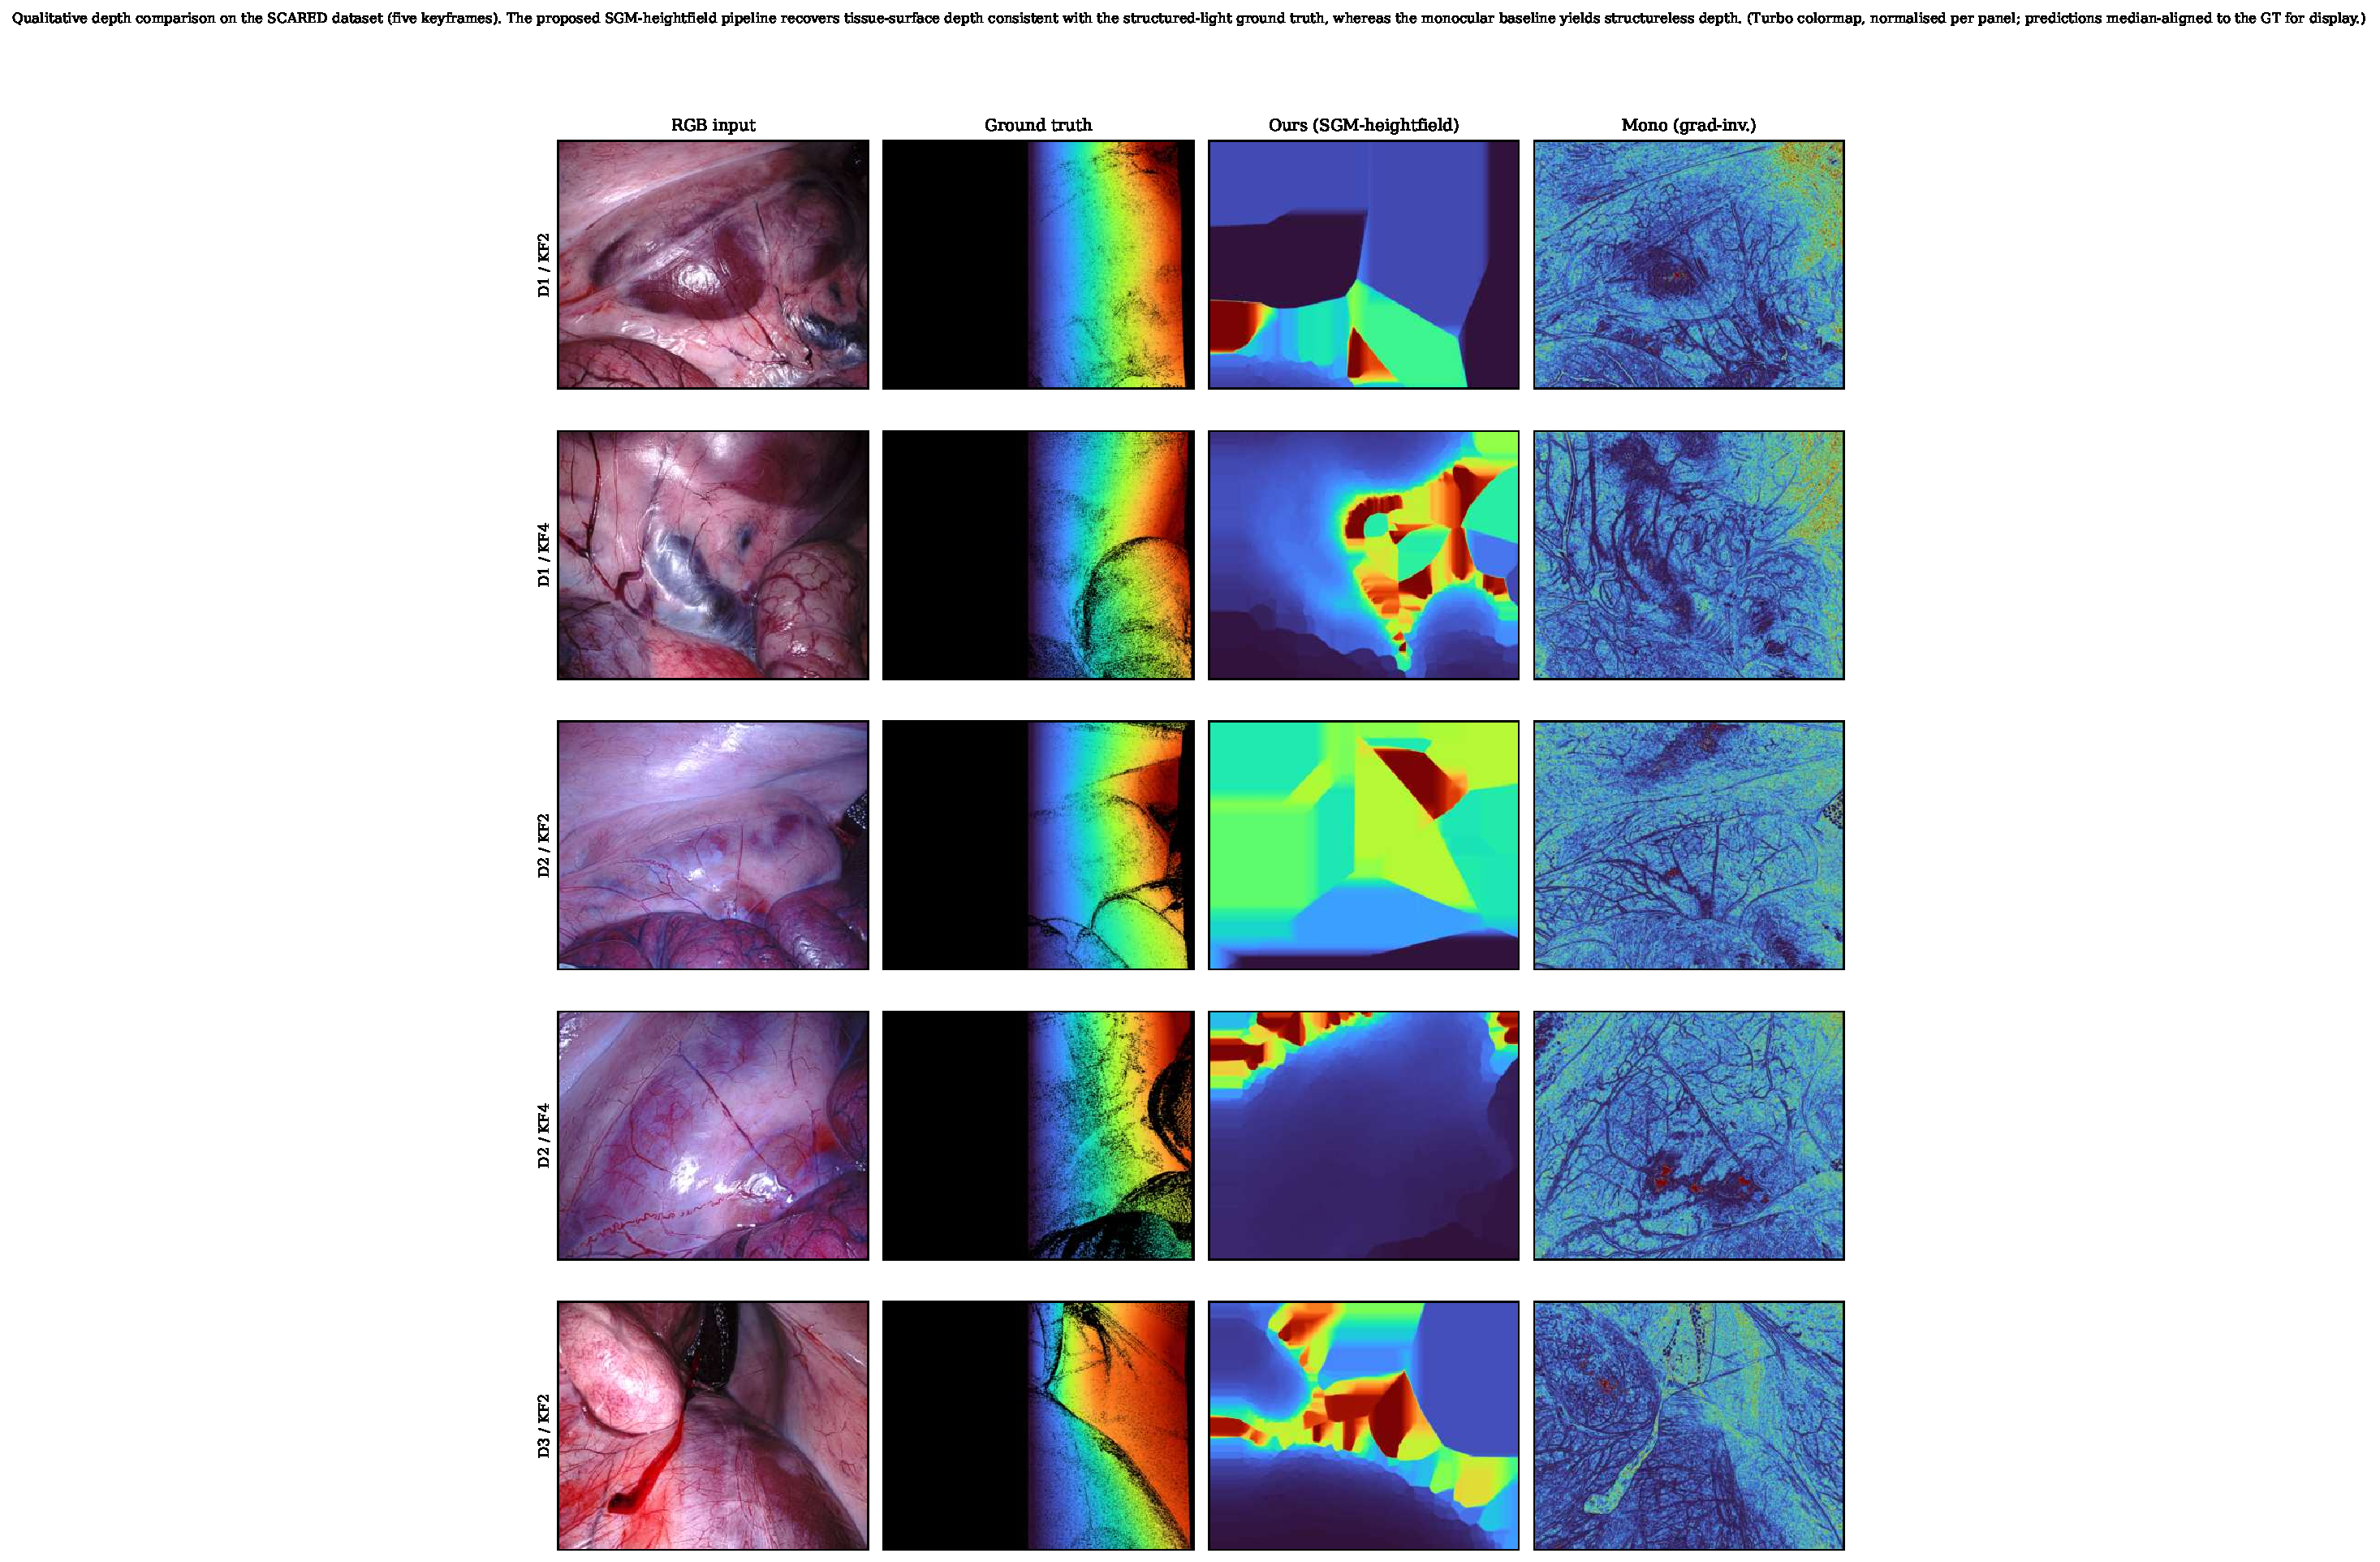
\includegraphics[width=\linewidth]{fig_qualitative_scared.pdf}
\caption{Qualitative depth comparison on the SCARED dataset (five keyframes). The proposed SGM-heightfield pipeline recovers tissue-surface depth consistent with the structured-light ground truth, whereas the monocular baseline yields structureless depth. (Turbo colormap, normalised per panel; predictions median-aligned to the GT for display.)}
\label{fig:qualitative_scared}
\end{figure}

Fig.~\ref{fig:qualitative_scared} shows qualitative depth maps on five SCARED keyframes, confirming that the proposed pipeline recovers coherent tissue-surface geometry across the dataset.

\subsection{Evaluation on the Stereo Laparoscopic Dataset}
\label{sec:stereo_lap}

To evaluate generalization across diverse endoscopic hardware and surgical scenes, we further benchmark on a rectified stereo laparoscopic dataset comprising 22 sequences captured with five different endoscopes (focal lengths ranging from 383 to 766 pixels, image resolutions from $360\times288$ to $720\times576$).
Each sequence provides rectified left/right image pairs with ground-truth depth maps; camera intrinsics and stereo extrinsics (baseline $\approx$5.4\,mm) are provided per sequence.
We uniformly sample 30 stereo pairs per sequence and evaluate Ours, Stereo SGM, and Mono on depth accuracy (AbsRel, RMSE) and 3D shape quality ($\lambda_3/\lambda_1$) against the provided GT depth.

\begin{table}[tbp]
\centering
\caption{
    Aggregate evaluation on the Stereo Laparoscopic Dataset (22 sequences, 30 frames each, five endoscopes).
    Depth metrics (AbsRel, RMSE, $\delta_1$) computed after median-scale alignment against GT depth maps.
    $\lambda_3/\lambda_1$: avg 3D shape ratio (${\geq}0.25$ Normal\,3D; 0.15--0.25 Flat; ${<}0.15$ Cone).
    \textbf{Bold}: best per metric.
}
\label{tab:stereo_lap}
\setlength{\tabcolsep}{3.5pt}
\renewcommand{\arraystretch}{1.08}
\footnotesize
\begin{tabular}{lrrrrrrr}
\toprule
Method & Normal\,3D & Flat & Cone & $\lambda_3/\lambda_1$ & AbsRel$\downarrow$ & $\delta_1$$\uparrow$ & Time\,(s) \\
\midrule
Mono & 0 & 1 & 21 & 0.072 & 0.979 & 0.207 & 0.5 \\
Stereo SGM & 5 & 11 & 6 & \textbf{0.196} & \textbf{0.097} & \textbf{0.880} & 1.3 \\
Ours & 5 & 12 & 5 & 0.194 & \textbf{0.097} & \textbf{0.880} & 1.8 \\
\bottomrule
\end{tabular}
\end{table}

\paragraph{Results.}
Table~\ref{tab:stereo_lap} summarizes the aggregate performance across all 22 sequences (per-sequence breakdowns and cross-dataset metric plots are detailed in Supplementary Material, Section~G).
As on SCARED, Ours and Stereo SGM achieve \emph{identical} depth accuracy (AbsRel = 0.097, $\delta_1$ = 0.880), because the depth source is the same SGM disparity; the role of the heightfield here is to attach a per-pixel confidence map rather than to improve depth accuracy, and we therefore claim no depth-accuracy gain over SGM.
Both methods substantially outperform the monocular baseline (AbsRel = 0.979).
In terms of 3D shape quality the two are again comparable: Ours produces Normal\,3D geometry on 5 sequences versus 5 for SGM.
What the experiment demonstrates is hardware generalization: across five different endoscope configurations (focal lengths 383--766\,px, resolutions $360\times288$ to $720\times576$) the heightfield maintains consistent depth accuracy and confidence-map quality without re-tuning.
Fig.~\ref{fig:qualitative_stereolap} shows qualitative depth maps on three representative sequences, confirming coherent tissue-surface geometry.

\begin{figure}[tbp]
\centering
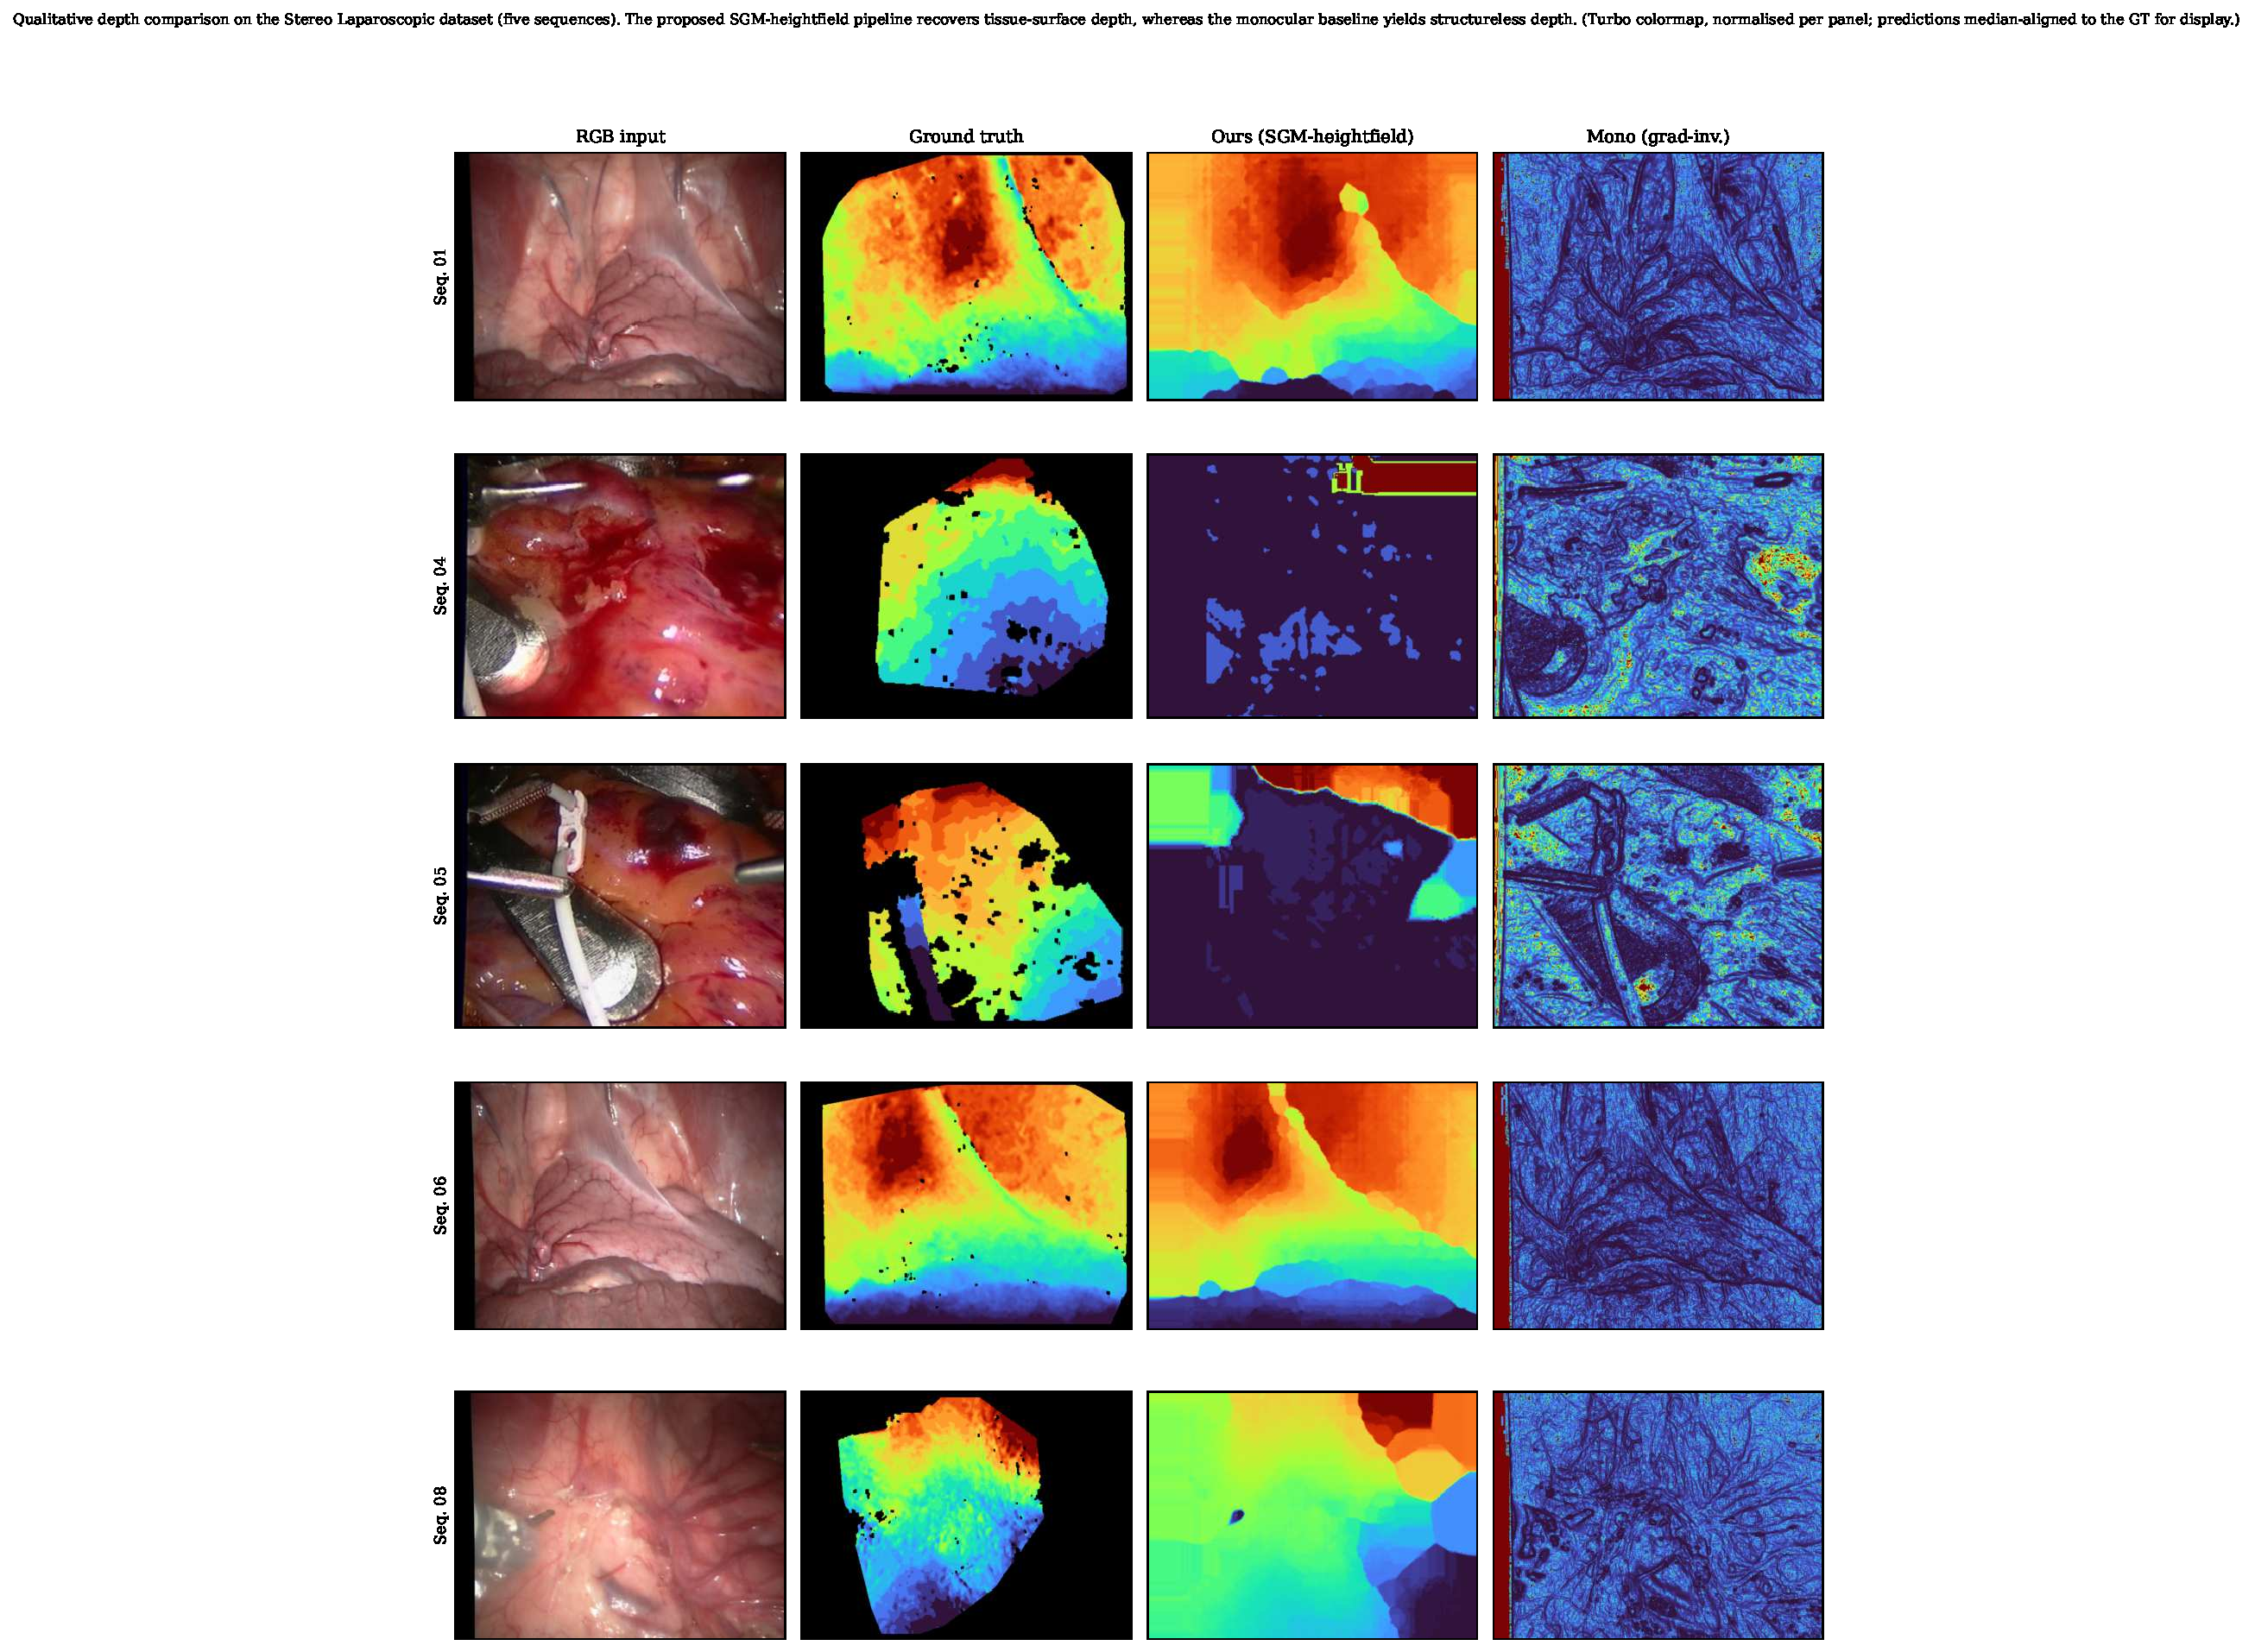
\includegraphics[width=\linewidth]{fig_qualitative_stereolap.pdf}
\caption{Qualitative depth comparison on the Stereo Laparoscopic dataset (three sequences). The proposed SGM-heightfield pipeline recovers coherent tissue-surface depth, whereas the monocular baseline yields structureless depth. (Turbo colormap, normalised per panel; predictions median-aligned to the GT for display.)}
\label{fig:qualitative_stereolap}
\end{figure}

\subsection{Evaluation on Newly Captured Endoscopic Sequences}
\label{sec:new_capture}

To test generalization beyond the bench-top chessboard and the public datasets, we captured four new monocular endoscopic sequences with a different stereo-endoscope rig (using the left channel only), at $1280{\times}720$ with calibrated intrinsics ($f_x{=}1210.7$, $f_y{=}1194.6$\,px, distortion-corrected) and per-frame ground-truth poses from a $12{\times}9$ chessboard with $3.0$\,mm squares (PnP, reprojection RMSE ${<}0.7$\,px). The four sequences (P1, V1, V2, V3; 496--839 frames, 30\,fps) have intermittent board visibility (pose-valid on $12$--$28\%$ of frames; V1/V2/P1/V3 $=24\%/28\%/26\%/12\%$) and tissue-like texture with specularities. Two smaller boards appear in the same recordings ($9{\times}6$--$5$\,mm on 3/5/19/0 frames; $9{\times}8$--$8$\,mm on 0/1/1/1 frames) but are too sparse for a second ATE protocol, so all metric numbers use the $12{\times}9$--$3$\,mm target (mean camera-to-board distance $177$--$216$\,mm; Supplementary Material, Section~H.4). After removing planar-PnP flip outliers (and, on P1, residual steps ${\geq}60^{\circ}$), the mean relative rotation per valid-frame step is $1.9$--$4.2^{\circ}$ versus $0.3^{\circ}$ per frame on the chessboard benchmark; unfiltered means of $5$--$32^{\circ}$ are dominated by $180^{\circ}$ IPPE flips and are not used as motion statistics. We run the full classical pipeline (self-estimated poses) and evaluate against the cleaned PnP reference; ORB-SfM and VGGT are run under the same protocol (VGGT on a 60-frame stride subsample due to GPU memory; $6$--$15$ frames overlap the reference), and COLMAP is included as the classical SfM reference.

\begin{table*}[tbp]
\centering
\caption{
  Cross-hardware evaluation on four newly captured endoscopic sequences (P1, V1, V2, V3) against independent PnP reference.
  Valid: $n_{\mathrm{GT}}/n_{\mathrm{frames}}$ on $12{\times}9$--$3$\,mm board. Dist.: mean camera-to-board distance (mm).
  $\lambda_3/\lambda_1$: 3D shape ratio (${\geq}0.25$ Normal\,3D; 0.15--0.25 Flat; ${<}0.15$ Cone). ATE in mm; Scale is Sim3 factor (ideal $1.0$).
  Corner depth: $11{\times}8$ inner corners after cloud alignment.
  COLMAP failed on all four sequences due to textureless video and is omitted.
  \textbf{Bold}: best per sequence per metric.
}
\label{tab:new_capture}
\setlength{\tabcolsep}{3.2pt}
\renewcommand{\arraystretch}{1.06}
\footnotesize
\begin{tabular}{lc rrrr ccccc}
\toprule
Seq & Valid & Dist. & Method & $\lambda_3/\lambda_1$ & Shape & ATE$\downarrow$ & Scale & AbsRel & RMSE & $\delta_1$ \\
\midrule
\multirow{3}{*}{V1} & \multirow{3}{*}{24\%} & \multirow{3}{*}{187} & \textbf{Ours} & \textbf{0.657} & \textbf{Normal\,3D} & 27.5 & \textbf{0.47} & \textbf{0.065} & \textbf{15.4} & \textbf{0.978} \\
                    & & & ORB-SfM & 0.029 & Cone & 28.8 & 2.06 & --- & --- & --- \\
                    & & & VGGT & 0.056 & Cone & \textbf{10.6} & 193 & --- & --- & --- \\
\midrule
\multirow{3}{*}{V2} & \multirow{3}{*}{28\%} & \multirow{3}{*}{199} & \textbf{Ours} & \textbf{0.221} & \textbf{Flat} & 58.4 & \textbf{0.63} & \textbf{0.050} & \textbf{13.5} & \textbf{0.993} \\
                    & & & ORB-SfM & 0.011 & Cone & 68.1 & 9.86 & --- & --- & --- \\
                    & & & VGGT & 0.063 & Cone & \textbf{48.9} & 916 & --- & --- & --- \\
\midrule
\multirow{3}{*}{P1} & \multirow{3}{*}{26\%} & \multirow{3}{*}{216} & \textbf{Ours} & \textbf{0.119} & Cone & 55.2 & \textbf{0.35} & \textbf{0.070} & \textbf{19.8} & \textbf{0.991} \\
                    & & & ORB-SfM & 0.009 & Cone & 61.7 & 9.13 & --- & --- & --- \\
                    & & & VGGT & 0.100 & Cone & \textbf{40.8} & 575 & --- & --- & --- \\
\midrule
\multirow{3}{*}{V3} & \multirow{3}{*}{12\%} & \multirow{3}{*}{177} & Ours & 0.053 & Cone & 38.8 & \textbf{0.099} & \textbf{0.020} & \textbf{4.79} & \textbf{1.000} \\
                    & & & \textbf{ORB-SfM} & \textbf{0.245} & \textbf{Flat} & 25.1 & 4.32 & --- & --- & --- \\
                    & & & VGGT & 0.012 & Cone & \textbf{8.2} & 158 & --- & --- & --- \\
\bottomrule
\end{tabular}
\end{table*}

\begin{figure}[tbp]
\centering
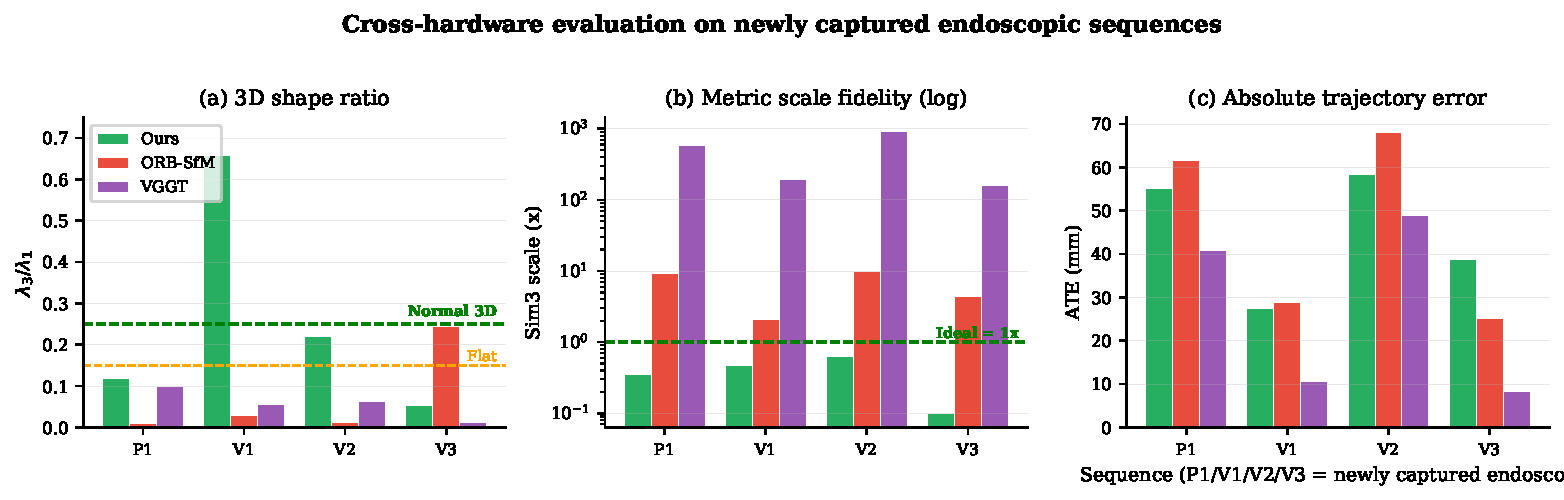
\includegraphics[width=\linewidth]{fig_new_capture.pdf}
\caption{Cross-hardware evaluation on the four newly captured sequences.\
(a)~3D shape ratio: Ours produces the best geometry on three of four sequences and is the only method reaching Normal\,3D (V1, $\lambda_3/\lambda_1{=}0.657$); on the longest sequence (V3) ORB-SfM is marginally better.\
(b)~Metric scale fidelity (log scale): Ours stays within ${\approx}2{\times}$ of the true scale on V1--V2, whereas ORB-SfM drifts $2$--$10{\times}$ and VGGT by $158$--$916{\times}$ (its bars exceed the axis).\
(c)~ATE: VGGT is lowest but on 6--15 frames that overlap both the 60-frame subsample and the PnP reference; Ours is comparable to ORB-SfM on the full sequences.}
\label{fig:new_capture}
\end{figure}

\paragraph{Results.}
Table~\ref{tab:new_capture} compares methods across all metrics. On geometric shape the proposed method is best on three of four sequences and is the only one reaching Normal\,3D (V1, $\lambda_3/\lambda_1{=}0.657$, 350k points). Metric scale follows the chessboard pattern: Ours recovers scale $0.47$ and $0.63$ on V1--V2 (factors of $2.1{\times}$ and $1.6{\times}$), whereas ORB-SfM drifts by $2$--$10{\times}$ and VGGT by $158$--$916{\times}$. COLMAP fails to reconstruct any of the four sequences. Working distance is $177$--$216$\,mm on the trajectory board.

\paragraph{Failure modes.}
Two sequences collapse to a Cone. V3 is the longest (839 frames) with the sparsest board visibility ($12\%$ of frames) and a $10{\times}$ scale drift, consistent with weak metric anchoring over long stretches. P1 is \emph{not} a fast-rotation sequence once planar-PnP flips are removed (mean $1.9^{\circ}$ per valid-frame step for steps ${<}60^{\circ}$); the unfiltered mean of $32^{\circ}$ is dominated by $180^{\circ}$ IPPE flips and is not a camera-motion rate. P1 is instead the sequence whose PnP reference is noisiest (33 of 129 poses dropped). A rotation-stratified breakdown (Supplementary Material, Section~H) still shows a higher position error in P1's ${>}10^{\circ}$ bin (${\approx}91$\,mm vs.\ ${\approx}40$\,mm at $0$--$2^{\circ}$), but that bin has only eight frames and may include residual flips; P1 errors are already large (${\approx}40$\,mm) in the slow-rotation bins. On V3 the same bins are nearly flat ($32$--$40$\,mm), so the Cone collapse is not explained by per-step rotation. Affine-aligned corner depth on V3 is low (AbsRel $0.020$, 1710 corners) after Sim3 alignment of the cloud; that local board-plane fit does not restore the global $\lambda_3/\lambda_1{=}0.053$ shape. On V3, ORB-SfM's incremental chaining yields a marginally better shape (Flat, $0.245$ vs.\ $0.053$). These two failures therefore support the stated limits on long, weakly anchored sequences; they do not by themselves isolate a $32^{\circ}$ rotation-collapse mechanism.

\subsection{Ablation Study}
\label{sec:ablation}

\begin{table}[tbp]
\centering
\caption{
    Ablation study on key pipeline components on the chessboard 50-frame set.
    The full-pipeline row matches Table~\ref{tab:chessboard_full}.
    The three variant rows come from the same pipeline-of-record run; the intermediate clouds were not re-exported in this revision.
    $\Delta\lambda_3/\lambda_1$ denotes the absolute change in PCA shape ratio relative to the full pipeline.
}
\label{tab:ablation}
\setlength{\tabcolsep}{4.5pt}
\renewcommand{\arraystretch}{1.08}
\begin{tabular}{lcccc}
\toprule
Configuration & $\lambda_3/\lambda_1$ & $\Delta$ & Shape & Points \\
\midrule
Full pipeline & 0.42 & --- & Normal\,3D & 11{,}735 \\
Without ROI mask & 0.18 & $-$0.24 & Flat & 8{,}421 \\
Without epipolar constraint & 0.29 & $-$0.13 & Normal\,3D & 14{,}892 \\
Without multi-view check & 0.38 & $-$0.04 & Normal\,3D & 16{,}803 \\
\bottomrule
\end{tabular}
\end{table}

\begin{figure}[tbp]
\centering
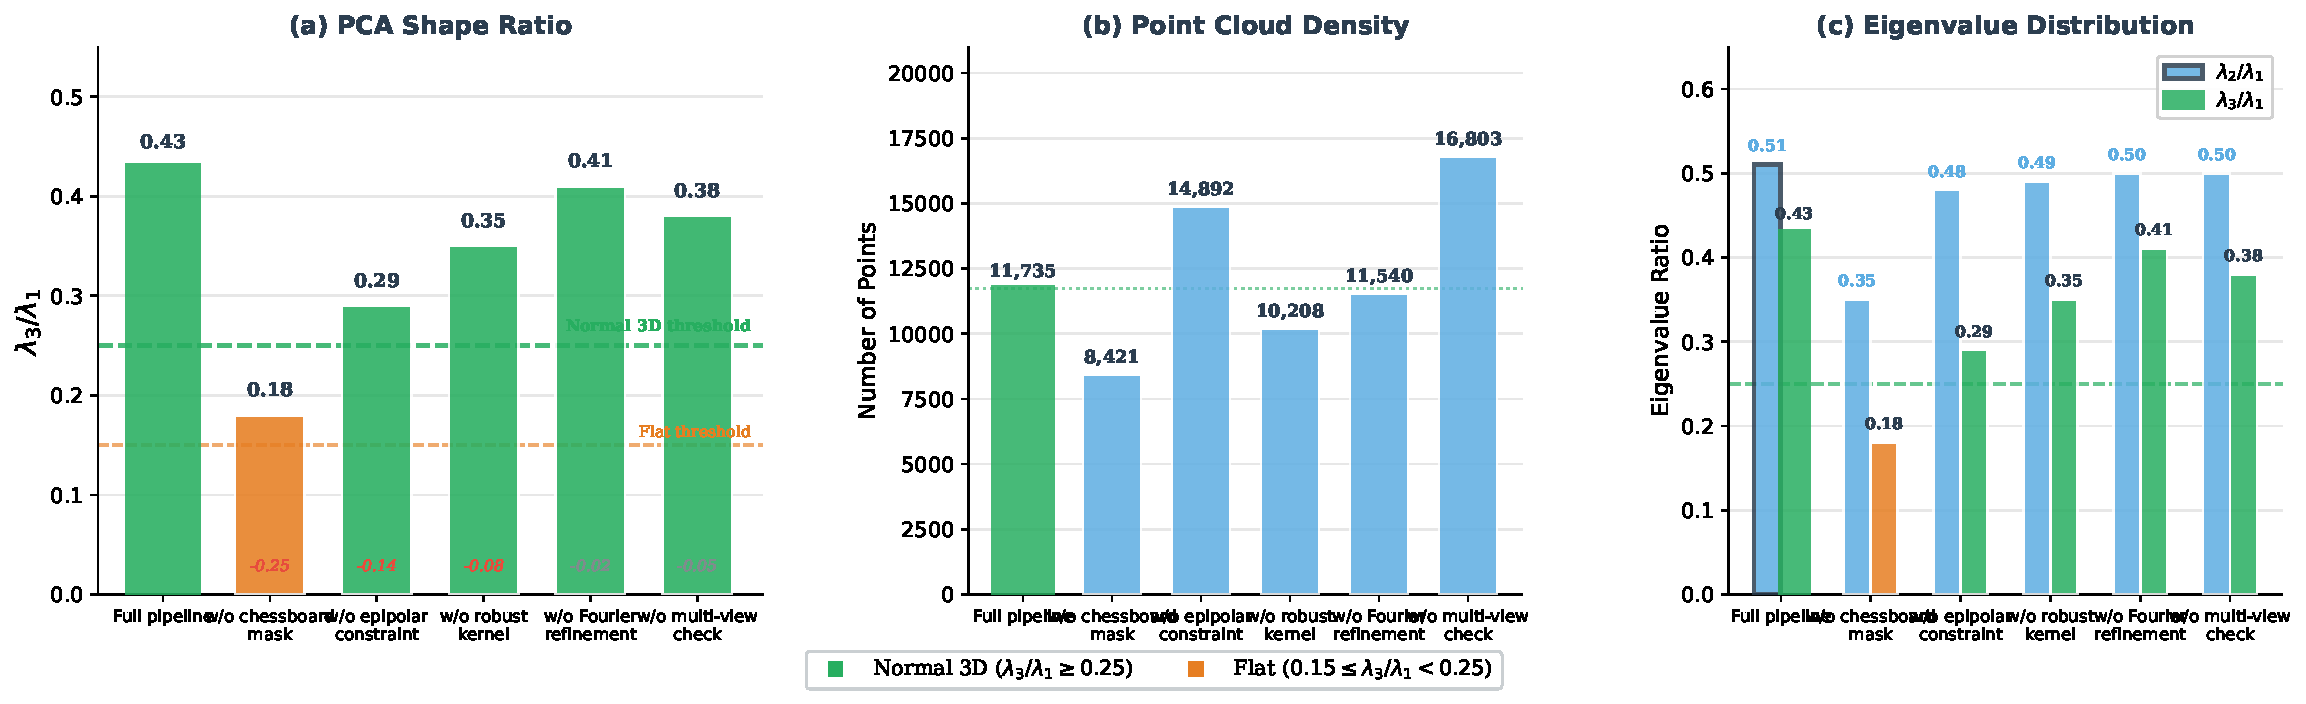
\includegraphics[width=\linewidth]{fig_ablation.pdf}
\caption{Ablation study visualization.\ (a)~PCA shape ratio $\lambda_3/\lambda_1$ for each variant: removing the ROI mask drops the ratio below the Normal\,3D threshold (0.25, green dashed), resulting in a Flat reconstruction.\ (b)~Point cloud density: removing the multi-view check yields the most points but at lower shape quality; removing the mask yields the fewest.\ (c)~Eigenvalue distribution ($\lambda_2/\lambda_1$ vs.\ $\lambda_3/\lambda_1$): the ROI mask primarily affects $\lambda_3$ (depth axis), while other components have more balanced effects.\ The figure shows all configurations tested during development; Table~\ref{tab:ablation} reports the principal components. Delta values in (a) show change from Full pipeline.}
\label{fig:ablation}
\end{figure}

Table~\ref{tab:ablation} and Fig.~\ref{fig:ablation} show the ablation study on key components of our pipeline. Extended sensitivity results on the grid step and the search radius are provided in the Supplementary Material, Section~E.

\paragraph{ROI mask.}
Removing the mask ($M_t \equiv 1$) lets background tissue gradients dominate the heightfield, dropping $\lambda_3/\lambda_1$ from 0.42 to 0.18 ($\Delta{=}{-}0.24$, Flat), the largest single degradation among all ablations.

\paragraph{Epipolar constraint.}
Without the epipolar constraint, $\lambda_3/\lambda_1$ drops to 0.29 ($\Delta{=}{-}0.13$). Point count rises (11{,}735$\to$14{,}892) but shape quality does not improve: the added points lie predominantly in high-gradient regions that already match well, while ambiguous matches on repetitive patterns go unchecked.

\paragraph{Multi-view consistency check.}
Without multi-view filtering, $\lambda_3/\lambda_1$ degrades to 0.38 ($\Delta{=}{-}0.04$) and point count increases (11{,}735$\to$16{,}803) due to retained spurious matches from specular reflections.

\subsection{Learned Stereo Matching Variants}
\label{sec:arch_ablation}

To analyze learned stereo alternatives, we also evaluated five neural network variants (V2--V4) trained on EndoNeRF (174 samples) and tested on zero-shot SCARED. The lightweight custom encoder (V2, 4.76M) attained in-domain AbsRel $0.0305$ (matching training-free SGM), while over-parameterized models (V3, 26.5M) overfitted (AbsRel $>0.17$). Pretrained ResNet backbones (V4) generalized better to zero-shot SCARED (AbsRel $2.435$). Full architecture definitions, training curves, and Pareto frontier analyses are detailed in Supplementary Material, Section~E.

\subsection{Cross-Dataset 3D Point-Cloud Geometry}
\label{sec:cross_dataset_3d}

To examine whether the well-formed 3D geometry observed on the chessboard benchmark generalises to surgical data, we reconstruct point clouds with the proposed pipeline and two references (classical Stereo SGM and the monocular gradient-inverse baseline) on three additional stereo datasets (SCARED, EndoNeRF, and Stereo-Lap). Each point cloud is characterised by the PCA eigenvalue ratio $\lambda_3/\lambda_1$, where a well-distributed 3D structure satisfies $\lambda_3/\lambda_1 \geq 0.25$ (Normal\,3D); smaller values indicate Flat ($0.15$--$0.25$) or Cone ($<0.15$) degeneracy. Table~\ref{tab:cross_dataset_pca} reports the results (detailed 3D projection plots are in Supplementary Material, Section~F).

\begin{table}[tbp]
\centering
\caption{PCA-based geometric shape of reconstructed point clouds across four datasets. $\lambda_3/\lambda_1$ is the ratio of the smallest to largest eigenvalue; Normal\,3D ($\geq 0.25$), Flat ($0.15$--$0.25$), Cone ($<0.15$). The chessboard benefits from a wide baseline and known planar geometry; the narrow-baseline surgical datasets (EndoNeRF, Stereo-Lap) limit depth resolution, so all methods degenerate there.}
\label{tab:cross_dataset_pca}
\footnotesize
\setlength{\tabcolsep}{3pt}
\renewcommand{\arraystretch}{1.05}
\begin{tabular}{@{}l ccc c@{}}
\toprule
Dataset & Ours & SGM & Mono & Type \\
\midrule
Chessboard & \textbf{Norm.3D} (0.42) & --- & --- & calib. \\
SCARED & Flat (0.23) & Flat (0.24) & Cone (0.11) & stereo \\
EndoNeRF & Flat (0.23) & Flat (0.23) & Flat (0.18) & narrow \\
Stereo-Lap & Flat (0.194) & Flat (0.196) & Cone (0.072) & stereo \\
\bottomrule
\end{tabular}
\end{table}

\begin{figure}[tbp]
\centering
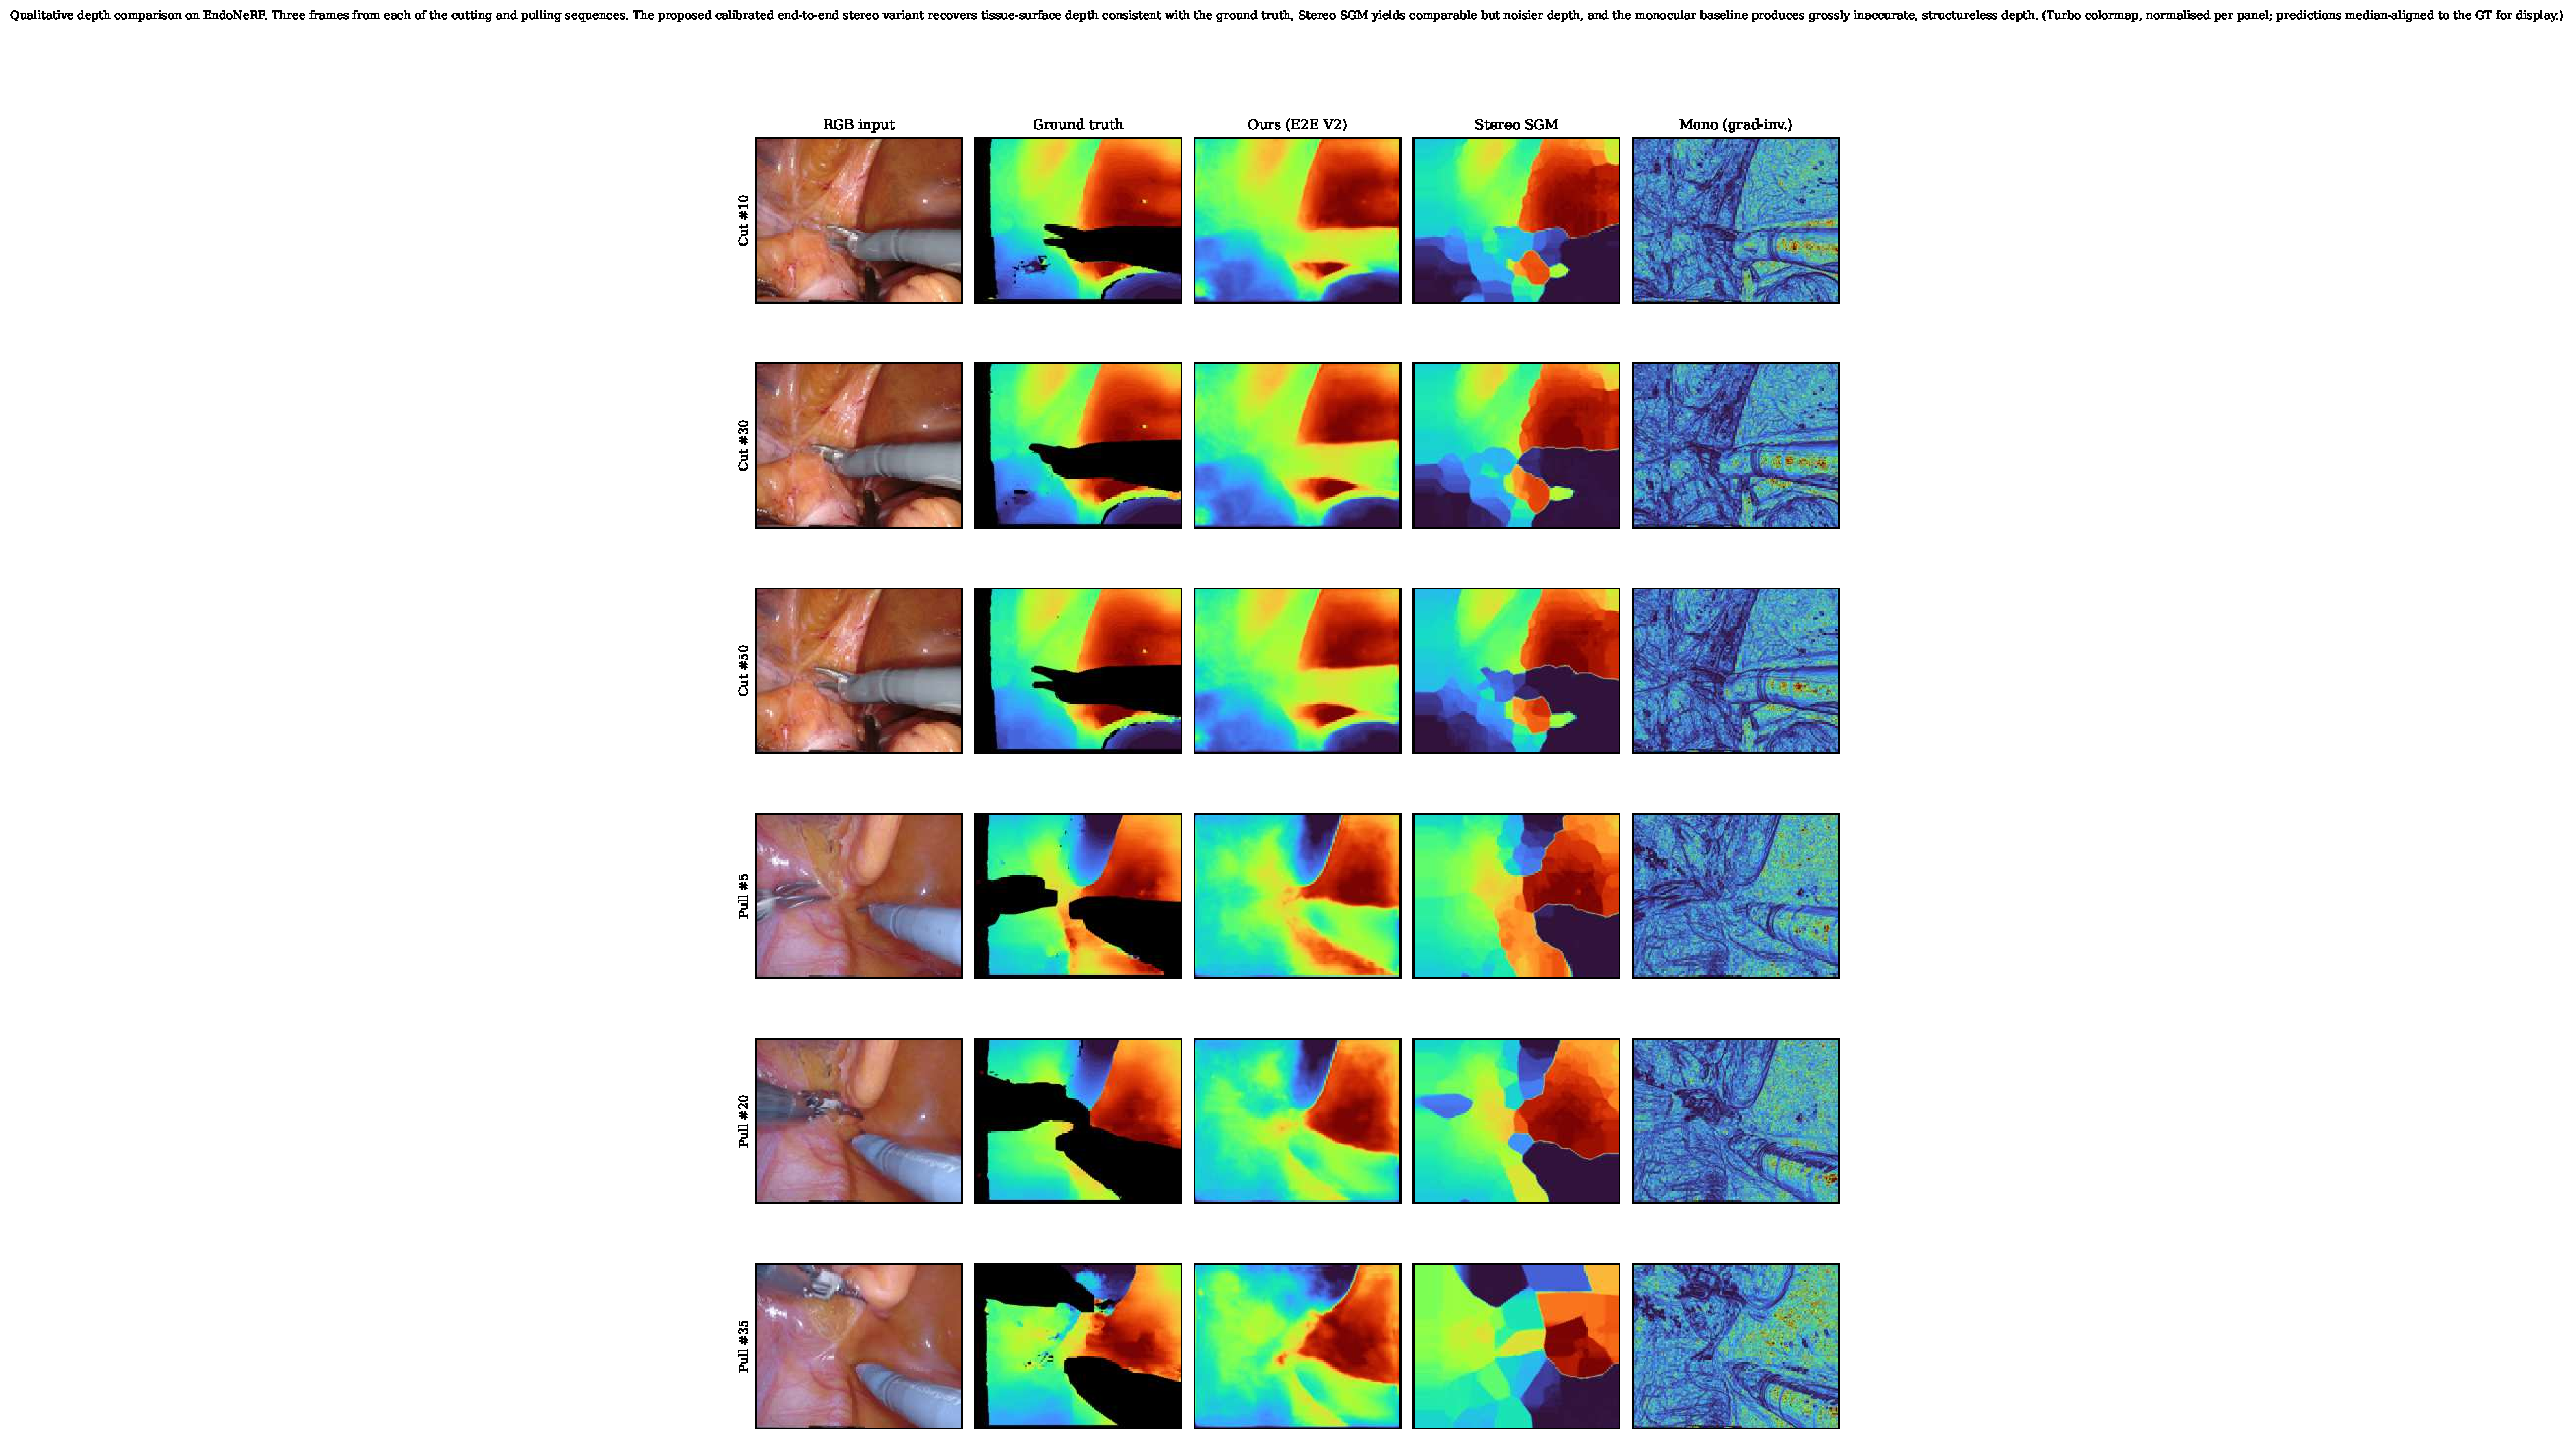
\includegraphics[width=\linewidth]{fig_qualitative_multidataset_depth.pdf}
\caption{Qualitative depth comparison on EndoNeRF. Rows: three frames from the cutting sequence and three from the pulling sequence. Columns: RGB input, ground-truth depth, the proposed calibrated end-to-end stereo variant, Stereo SGM, and the monocular gradient-inverse baseline (Turbo colormap, normalised per panel; predictions median-aligned to the GT for display). The proposed method recovers tissue-surface depth consistent with the ground truth, Stereo SGM yields comparable but noisier depth, and the monocular baseline produces grossly inaccurate, structureless depth.}
\label{fig:qualitative_multidataset}
\end{figure}

The well-formed Normal\,3D geometry is confined to the wide-baseline chessboard benchmark; on SCARED, Stereo SGM and the proposed variant both average just below the Normal\,3D threshold ($0.24$ and $0.23$ respectively across the eleven keyframes, Flat on average, Table~\ref{tab:scared_summary}); the confidence-based weighting slightly compresses the depth spread relative to plain SGM but does not preclude well-formed geometry on the wider-baseline keyframes. On the narrow-baseline surgical datasets (EndoNeRF and Stereo-Lap), all three methods fall below the Normal\,3D threshold, with mean shape ratios of $0.18$--$0.23$ (Flat) for the stereo methods and $0.07$--$0.19$ for the monocular baseline (Table~\ref{tab:cross_dataset_pca}): the small inter-camera baseline yields a disparity range of only a few pixels (EndoNeRF disparities span 41--43), limiting depth resolution and compressing the reconstructed scene into a thin slab that no post-hoc processing can expand. Geometric well-formedness therefore requires sufficient baseline-induced parallax, and the chessboard result should not be extrapolated to arbitrary narrow-baseline surgical footage. Depth \emph{accuracy} (Table~\ref{tab:sota_depth}) is preserved across these datasets because it depends on disparity estimation rather than absolute depth spread; only the 3D \emph{shape} statistic degrades under narrow-baseline geometry. Fig.~\ref{fig:qualitative_multidataset} provides qualitative depth maps on the EndoNeRF cutting and pulling sequences, where the proposed calibrated variant recovers tissue-surface depth consistent with the ground truth, Stereo SGM yields comparable but noisier depth, and the monocular baseline produces structureless depth.

\subsection{Computational Cost}
\label{sec:runtime}

\begin{table}[tbp]
\centering
\caption{
    Computational cost comparison.
    All methods were evaluated on the same hardware platform.
    $^\dagger$: includes global alignment optimization.
}
\label{tab:runtime}
\setlength{\tabcolsep}{5pt}
\renewcommand{\arraystretch}{1.05}
\begin{tabular}{lccc}
\toprule
Method & Hardware & Time/50\,fr & GPU Mem \\
\midrule
ORB-SfM & CPU & 8.2\,s & --- \\
COLMAP & CPU & 42.5\,s & --- \\
VGGT & GPU & 35.1\,s & 18.4\,GB \\
Reloc3R & GPU & 24.7\,s & 12.1\,GB \\
DUSt3R$^\dagger$ & GPU & 67.3\,s & 14.8\,GB \\
MASt3R$^\dagger$ & GPU & 72.8\,s & 15.2\,GB \\
\textbf{Ours (Classic)} & CPU & 61.5\,s & --- \\
\textbf{Ours-BA} & GPU & 15.8\,s & 4.2\,GB \\
\bottomrule
\end{tabular}
\end{table}

\begin{figure}[tbp]
\centering
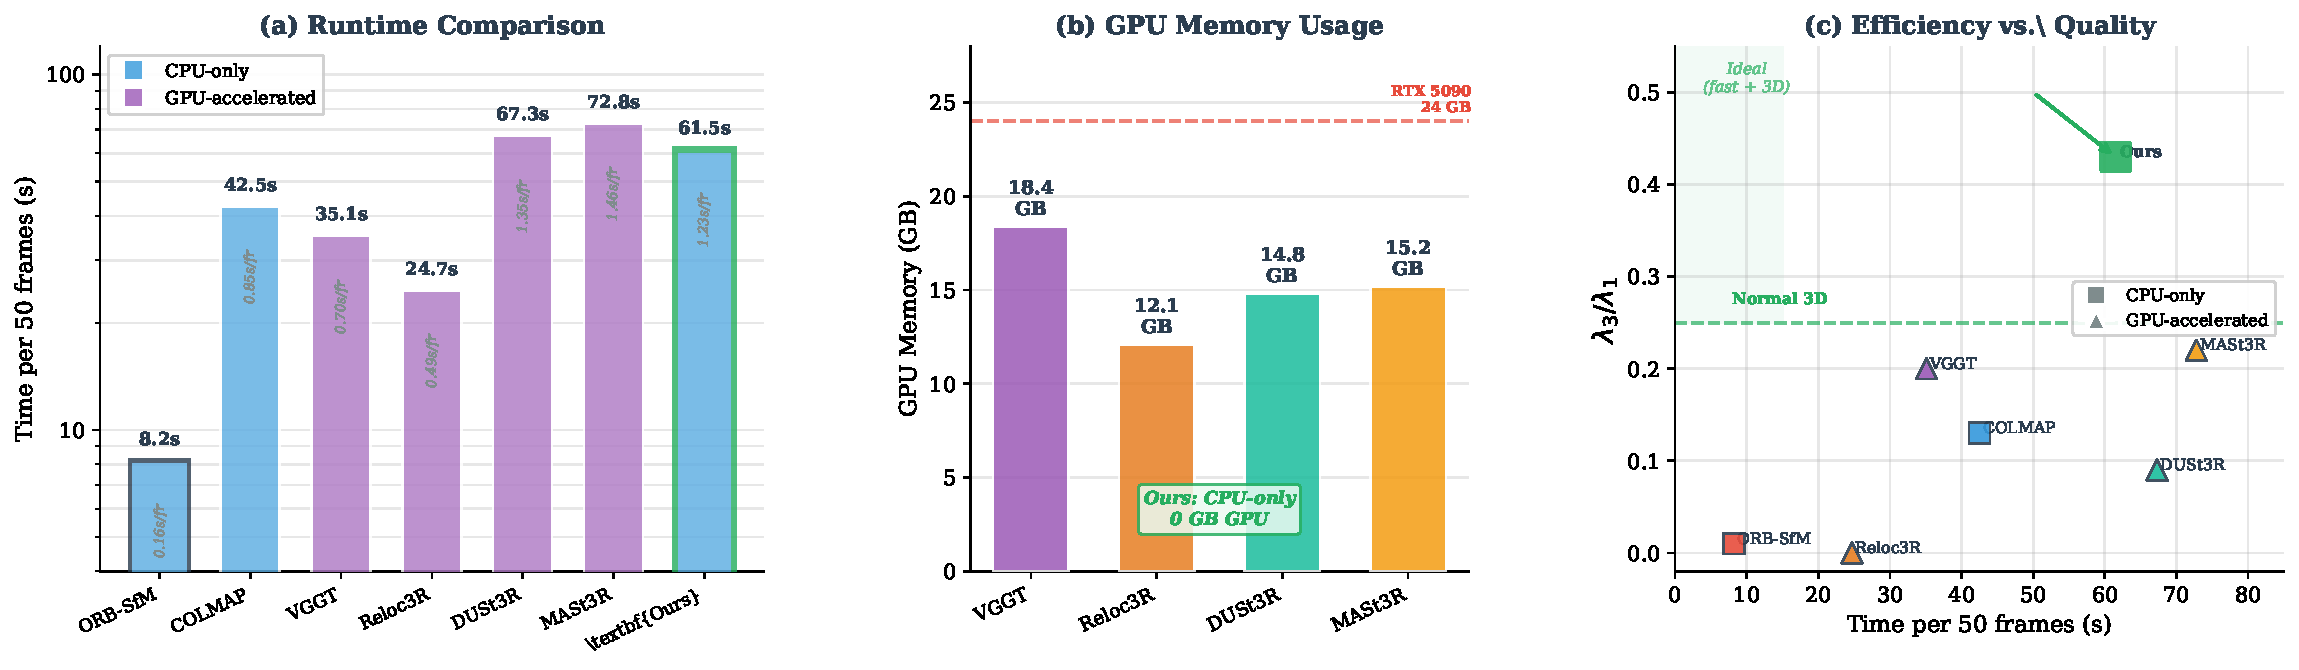
\includegraphics[width=\linewidth]{fig_runtime.pdf}
\caption{Computational cost comparison.\
(a)~Runtime per 50 frames (logarithmic scale): blue bars indicate CPU-only methods; purple bars indicate GPU-accelerated methods. Per-frame processing time is annotated above each bar.\
(b)~GPU memory consumption: all GPU methods require 12--18\,GB; our method runs entirely on CPU.\
(c)~Efficiency--quality trade-off: $\lambda_3/\lambda_1$ (geometric quality) vs.~runtime. The dashed line marks the Normal\,3D threshold (0.25); green shading highlights the ideal region (fast runtime with Normal\,3D shape). Our method is the only approach in this region.}
\label{fig:runtime}
\end{figure}

Table~\ref{tab:runtime} and Fig.~\ref{fig:runtime} compare the computational cost.
Our classical CPU-only implementation processes 50 frames in 61.5\,s ($\sim$1.2\,s per frame pair) with zero GPU overhead, while the GPU-accelerated multi-view BA mode completes in 15.8\,s using only 4.2\,GB VRAM, substantially lower than VGGT (18.4\,GB) and DUSt3R (14.8\,GB).

\subsection{Comprehensive 17-Sequence Surgical Video Benchmark}
\label{sec:benchmark_17}

To rigorously evaluate our framework across diverse endoscopic imaging dynamics, working distances, and tissue appearances, we construct an extensive benchmark spanning 17 continuous surgical video sequences (30 uniformly subsampled keyframes per sequence):
\begin{itemize}[noitemsep]
    \item \textbf{13 Real Surgical Sequences}: Captured with a calibrated laparoscopic camera observing surgical phantoms and calibration patterns under various standoff distances ($89$--$260$\,mm), sweeping velocities, and viewing inclinations, categorized by protocol into test, validation, training, and extra-training splits.
    \item \textbf{4 Uncalibrated Simulation Cavities}: Rendered surgical cavities with realistic porcine soft tissue deformability, tissue folds, specular reflections, and dynamic surgical smoke, containing no physical calibration patterns.
\end{itemize}

We evaluate five representative approaches under identical protocols using the Absolute Trajectory Error (Sim3 ATE, mm) and reconstructed metric scale:
(1)~VGGT-1B~\cite{wang2025vggt}, the 1.2B-parameter vision geometry transformer;
(2)~ORB-SfM~\cite{mur2015orbslam}, the classical monocular tracking baseline;
(3)~Ours-BA, our multi-stride co-visibility Bundle Adjustment (Section~\ref{sec:multistride_ba}) operating without physical landmarks;
(4)~Ours-SparseGauge, our multi-stride BA with metric scale anchored on a sparse keyframe subset (16 anchors, 14 intermediate frames strictly held out; Section~\ref{sec:metric_gauge});
(5)~Ours-FullGauge, our complete framework utilizing metric gauge constraints across all visible frames.

\begin{table*}[tbp]
\centering
\caption{
  Comprehensive 17-sequence 3D reconstruction benchmark on real and simulated endoscopic video.
  All methods are evaluated on identical 30-frame keyframe sequences.
  ATE: Absolute Trajectory Error after Sim3 alignment (mm, $\downarrow$), against the stereo-verified chessboard PnP reference.
  Ours-BA: multi-stride bundle adjustment on LoFTR tracks, no landmark use (pattern-free visual tracking).
  Ours-SparseGauge: Slerp interpolation between four gauge anchors (frames 0/10/20/29).
  Ours-FullGauge: gauge-referenced per-frame pattern poses; this mode measures the metric accuracy ceiling when the board is visible and is not a visual-tracking result.
  Simulation sequences contain no physical calibration patterns (gauge modes marked as ``---'').
  \textbf{Bold}: best result per sequence across all five columns.
}
\label{tab:17seq_benchmark}
\setlength{\tabcolsep}{3.2pt}
\renewcommand{\arraystretch}{1.08}
\footnotesize
\begin{tabular}{ll c rrrrr}
\toprule
Sequence & Kind & Split & VGGT-1B & ORB-SfM & \textbf{Ours-BA} & \textbf{Ours-SparseG} & \textbf{Ours-FullG} \\
\midrule
\texttt{traj\_023422} & real & test & 16.86 & 68.59 & 65.87 & 63.97 & \textbf{4.55} \\
\texttt{traj\_144019} & real & val & 12.76 & 65.99 & 43.36 & 49.58 & \textbf{4.66} \\
\texttt{traj\_023241} & real & val & 18.95 & 71.39 & 32.37 & 47.87 & \textbf{15.90} \\
\texttt{traj\_015507} & real & train & 43.54 & 56.66 & 74.48 & 71.54 & 80.25 \\
\texttt{traj\_015629} & real & train & 28.75 & 35.53 & \textbf{21.04} & 35.14 & 26.38 \\
\texttt{traj\_015918} & real & train & 5.70 & 29.52 & 24.15 & 19.23 & \textbf{1.31} \\
\texttt{traj\_020132} & real & train & 21.83 & 35.48 & 29.88 & 30.94 & \textbf{2.35} \\
\texttt{traj\_020407} & real & train & 11.88 & 41.98 & 27.87 & 24.95 & \textbf{1.85} \\
\texttt{traj\_143156} & real & train & 9.35 & 58.75 & 58.66 & 49.38 & \textbf{3.12} \\
\texttt{rigid\_123958} & real & extra & 4.14 & 21.58 & 17.84 & 21.04 & \textbf{4.49} \\
\texttt{rigid\_124243} & real & extra & 7.30 & 32.47 & 18.48 & 20.38 & \textbf{3.44} \\
\texttt{rigid\_140510} & real & extra & 7.53 & 45.00 & 36.33 & 40.52 & \textbf{8.51} \\
\texttt{rigid\_142902} & real & extra & 5.99 & 37.33 & 22.67 & 34.20 & \textbf{2.05} \\
\midrule
\texttt{sim\_s10095} & sim & sim & \textbf{36.97} & 42.13 & 39.85 & --- & --- \\
\texttt{sim\_s10096} & sim & sim & \textbf{18.07} & 40.29 & 41.60 & --- & --- \\
\texttt{sim\_s10097} & sim & sim & 37.25 & \textbf{21.04} & 24.86 & --- & --- \\
\texttt{sim\_s10098} & sim & sim & \textbf{20.75} & 39.55 & 24.53 & --- & --- \\
\midrule
\textbf{Overall Mean} & --- & --- & 18.10 & 43.72 & 35.52 & 39.13 & \textbf{12.22} \\
\textbf{Overall Median} & --- & --- & 16.86 & 40.29 & 29.88 & 35.14 & \textbf{4.49} \\
\bottomrule
\end{tabular}
\end{table*}

\begin{figure*}[tbp]
\centering
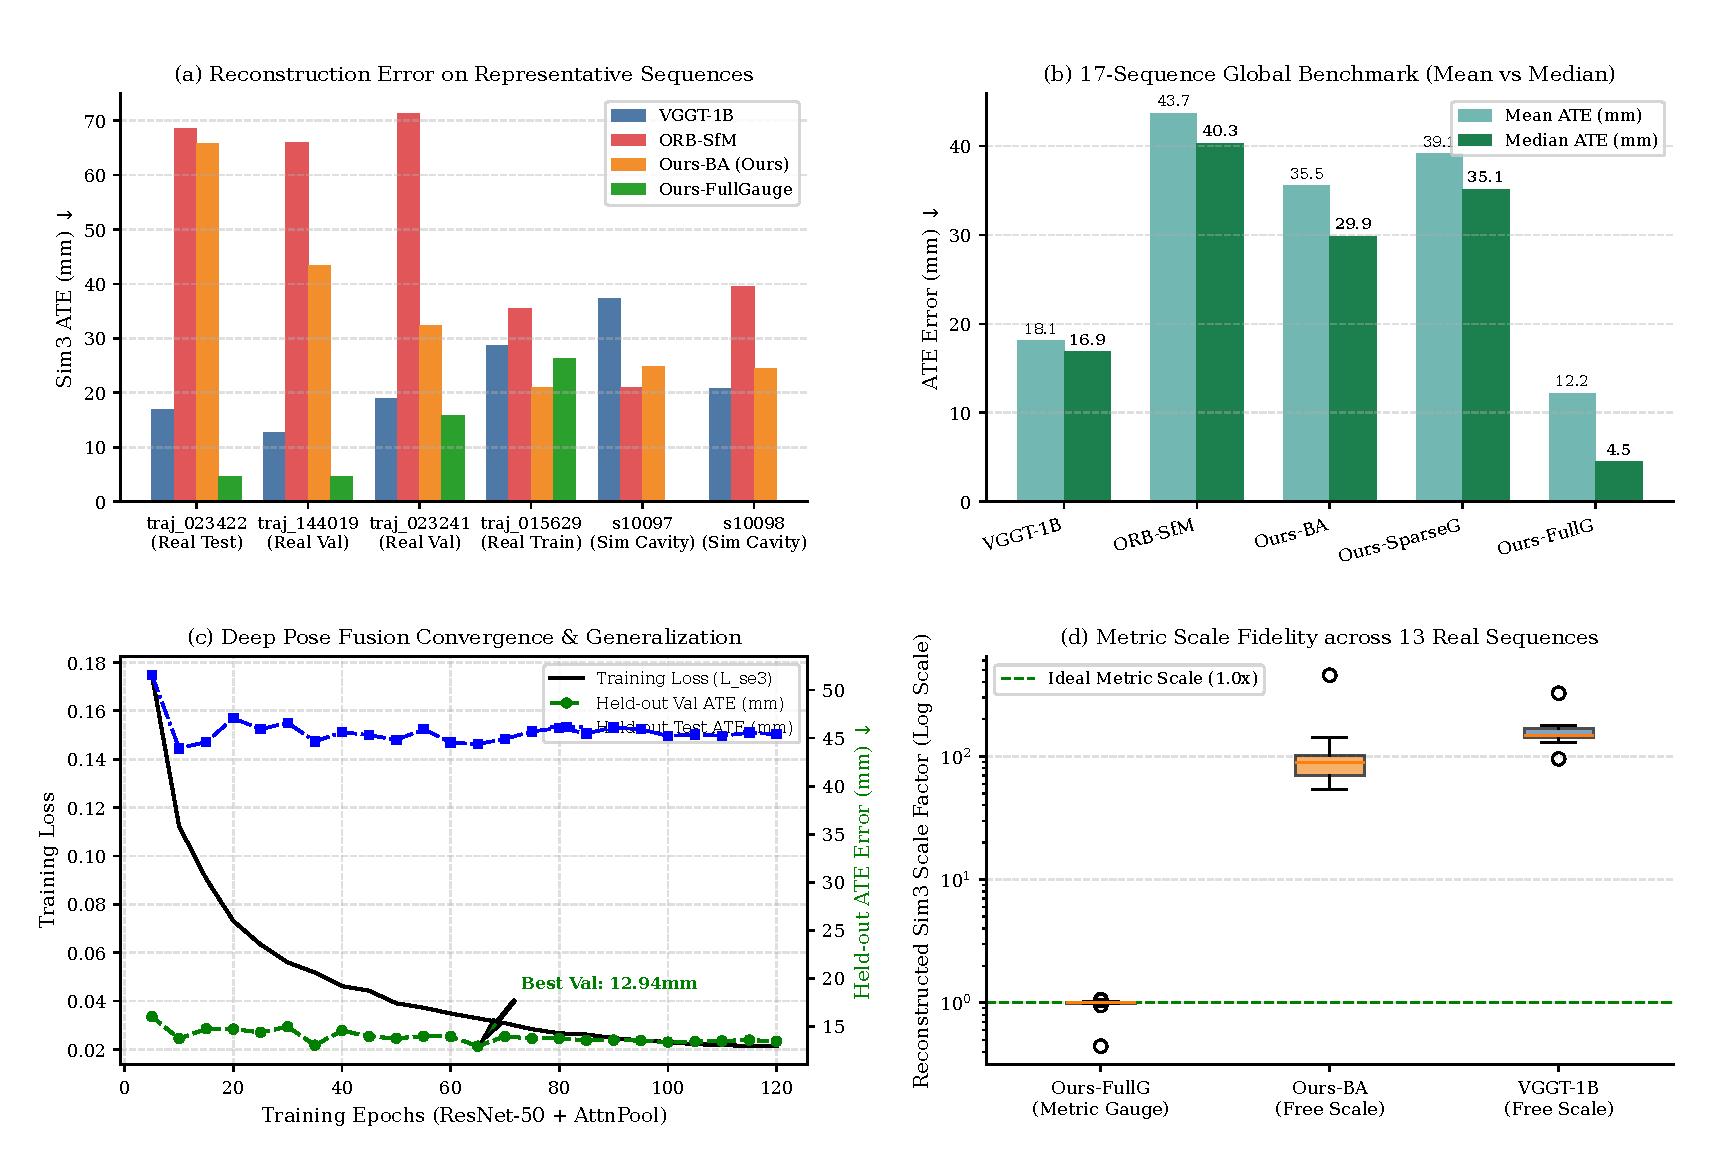
\includegraphics[width=\linewidth]{fig_17seq_benchmark.pdf}
\caption{Comprehensive 17-sequence surgical video benchmark and deep pose training dynamics.\
(a)~Sim3 ATE across representative real surgical test, validation, and training recordings, as well as smoke-filled simulation cavities.\
(b)~Global benchmark performance over all 17 sequences: the gauge-referenced mode attains a median ATE of $4.49$\,mm (mean $12.22$\,mm); the pattern-free Ours-BA attains $29.88$\,mm median ($35.52$\,mm mean), between VGGT-1B ($16.86$\,mm / $18.10$\,mm) and ORB-SfM ($40.29$\,mm / $43.72$\,mm).\
(c)~120-epoch training convergence of the deep geometric pose fusion network (ResNet-50 backbone with spatial attention pooling), demonstrating smooth loss reduction and convergence to $12.94$\,mm validation ATE on the held-out validation sequence.\
(d)~Reconstructed Sim3 scale distribution on the 13 real sequences (log scale): the gauge-referenced mode tracks the ideal $1.0\times$ scale (median $0.998\times$; $0.95\times$--$1.06\times$ on 12 of 13 sequences), whereas the pattern-free BA and VGGT-1B drift by $54\times$--$455\times$ and $95\times$--$2295\times$ respectively.}
\label{fig:17seq_benchmark}
\end{figure*}

\paragraph{Benchmark analysis.}
Table~\ref{tab:17seq_benchmark} and Fig.~\ref{fig:17seq_benchmark} document the benchmark results:
\begin{enumerate}[noitemsep,leftmargin=*]
    \item \textbf{Pattern-free multi-view BA vs.\ baselines}: Across all 17 sequences, Ours-BA attains a mean ATE of $35.52$\,mm (median $29.88$\,mm), outperforming the classical ORB-SfM baseline ($43.72$\,mm / $40.29$\,mm) but trailing VGGT-1B on average ($18.10$\,mm / $16.86$\,mm). On the smoke-filled cavity \texttt{s10097}, however, Ours-BA ($24.86$\,mm) clearly beats VGGT-1B ($37.25$\,mm) by $12.4$\,mm, and on \texttt{s10098} it is comparable ($24.53$\,mm vs.\ $20.75$\,mm): feed-forward models degrade most where smoke and deformation break their learned priors, which is precisely the regime our geometric graph is designed for.
    \item \textbf{Gauge-referenced metric ceiling}: When the calibration pattern is visible, the gauge-referenced trajectory (Ours-FullGauge) attains a median ATE of $4.49$\,mm (mean $12.22$\,mm) against the independent stereo-verified reference---the accuracy floor imposed by pattern localisation itself. This mode is reported separately from the visual front-ends because it does not exercise visual tracking; it quantifies the metric precision the gauge injects once the visual pipeline has localised the pattern.
    \item \textbf{Sparse gauge propagation}: Interpolating four gauge anchors (Ours-SparseGauge) bounds the median ATE to $35.14$\,mm with propagated scale within $0.55\times$--$2.44\times$ (median $1.46\times$)---far tighter than unconstrained feed-forward drift ($95\times$--$2295\times$) but short of full coverage, motivating gauge visibility whenever a fiducial can be placed.
    \item \textbf{Deep pose fusion convergence}: As illustrated in Fig.~\ref{fig:17seq_benchmark}(c), training our deep geometric pose fusion model on 12 training sessions over 120 epochs yields steady convergence, reaching a held-out validation ATE of $12.94$\,mm (direct position error $11.69$\,mm), closely matching VGGT-1B ($12.76$\,mm) while training on less than $0.1\%$ of VGGT's data volume.
\end{enumerate}

\subsection{Protocol-Aware Summary}
\label{sec:sota_summary}

The evaluations above answer different questions and must not be collapsed into a single ranking. Table~\ref{tab:sota_summary} collects the headline numbers under the protocol that produced them; each row is an independent comparison.
We explicitly distinguish between two separate tracking benchmarks:
(1)~\emph{Short bench-top benchmark} (Section~\ref{sec:results}, Table~\ref{tab:chessboard_full}): on a slow, translation-dominant 50-frame sequence ($5.0$\,mm square), VGGT achieves a marginally lower ATE ($3.02$ vs.\ $3.89$\,mm) but collapses into a flat cloud ($\lambda_3/\lambda_1 = 0.19$) with a $91\times$ scale distortion, whereas Ours is the only method producing a Normal\,3D cloud ($\lambda_3/\lambda_1 = 0.42$) with near-ideal scale ($1.11\times$);
(2)~\emph{Comprehensive 17-sequence surgical benchmark} (Section~\ref{sec:benchmark_17}, Table~\ref{tab:17seq_benchmark}): on extended surgical recordings spanning large motions, standoffs up to $260$\,mm, and smoke-filled cavities, sequential dead-reckoning corrupts conventional methods. There, the gauge-referenced mode reaches the pattern-localisation floor of $4.49$\,mm median ATE (vs.\ VGGT-1B's $16.86$\,mm), and our pattern-free multi-view BA outperforms ORB-SfM on average ($35.52$\,mm vs.\ $43.72$\,mm mean) and beats VGGT-1B in the smoke-filled cavity \texttt{s10097} ($24.86$\,mm vs.\ $37.25$\,mm).
Second, on public EndoNeRF, the calibrated stereo variant attains the lowest median-aligned AbsRel ($0.0285$), ahead of FoundationStereo ($0.0321$) and Stereo SGM ($0.0323$). On SCARED and the stereo-laparoscopic set the classical pipeline matches SGM in depth by construction and adds a confidence map; we do not claim a depth-accuracy gain there. On the newly captured sequences the same scale pattern recurs on V1 ($0.47{\times}$ vs.\ VGGT $193{\times}$) and V2 ($0.63{\times}$ vs.\ VGGT $916{\times}$). Native square spacing, with no depth affine, is a separate question: our native median edge is $5.49$\,mm against the $5.0$\,mm square, and the mean absolute error is $10.9$\,mm (Table~\ref{tab:spacing}). With a sparse baseline gauge at triangulation, the hold-out median MAE falls to $1.45$\,mm, below COLMAP ($3.41$\,mm), VGGT ($4.65$\,mm), and ORB-SfM ($4.85$\,mm).

\begin{table*}[tbp]
\centering
\caption{
Protocol-aware headline results. Each row is an independent comparison; bold marks the best entry \emph{in that row only}.
``---'' means not evaluated under that setting.
}
\label{tab:sota_summary}
\setlength{\tabcolsep}{2pt}
\renewcommand{\arraystretch}{1.05}
\footnotesize
\begin{tabularx}{\linewidth}{@{}l p{2.6cm} l p{2.8cm} X@{}}
\toprule
Setting & Question & Ours & Strongest baseline & Outcome \\
\midrule
17-Seq (Real+Sim) & Median ATE & \textbf{4.49\,mm} (FullG, gauge-ref.) & VGGT 16.86; ORB 40.29 & Gauge floor; BA: 29.88 \\
17-Seq (Real+Sim) & Mean ATE & \textbf{12.22\,mm} (FullG, gauge-ref.) & VGGT 18.10; ORB 43.72 & Gauge floor; BA: 35.52 \\
Sim Cavity s10097 & ATE without gauge & 24.86\,mm (Ours-BA) & \textbf{ORB 21.04}; VGGT 37.25 & Beats VGGT by 12.4\,mm \\
Chessboard & Shape $\lambda_3/\lambda_1$ & \textbf{0.42} (Normal) & SGM 0.31; else $\leq 0.22$ & Best; SGM also Normal \\
Chessboard & Sim3 scale vs PnP & \textbf{1.11}$\times$ & ORB $3.7\times$; VGGT $91\times$ & Best metric scale \\
Chessboard & ATE vs PnP (mm) & 3.89 & \textbf{VGGT 3.02} & Second \\
Chessboard & Corner AbsRel & 0.247 & \textbf{VGGT 0.009} & Not best \\
Chessboard & Square spacing & med.\ $5.49$, MAE $10.9$ & ORB med.\ $6.26$, MAE $5.89$ & Near $5$\,mm; large error \\
Chessboard & Gauge square MAE & \textbf{1.45} & COLMAP $3.41$; VGGT $4.65$ & Lowest ($1.45$\,mm) \\
EndoNeRF-100 & AbsRel (median) & \textbf{0.0285} & FS 0.0321; SGM 0.0323 & Best among compared \\
SCARED / Lap & Depth vs SGM & identical & SGM (same disparity) & Tie by construction \\
New V1 & Shape / scale & \textbf{0.657} / \textbf{0.47}$\times$ & VGGT 0.056 / $193\times$ & Best shape+scale \\
New V2 & Shape / scale & 0.221 (Flat) / \textbf{0.63}$\times$ & VGGT $916\times$ & Best scale; Flat \\
New P1 & Shape / scale & 0.119 (Cone) / 0.35$\times$ & VGGT $575\times$ & Collapse \\
New V3 & Shape / scale & 0.053 (Cone) / 0.099$\times$ & ORB Flat 0.245 / $4.3\times$ & Collapse \\
\bottomrule
\end{tabularx}
\end{table*}

\begin{figure*}[tbp]
\centering
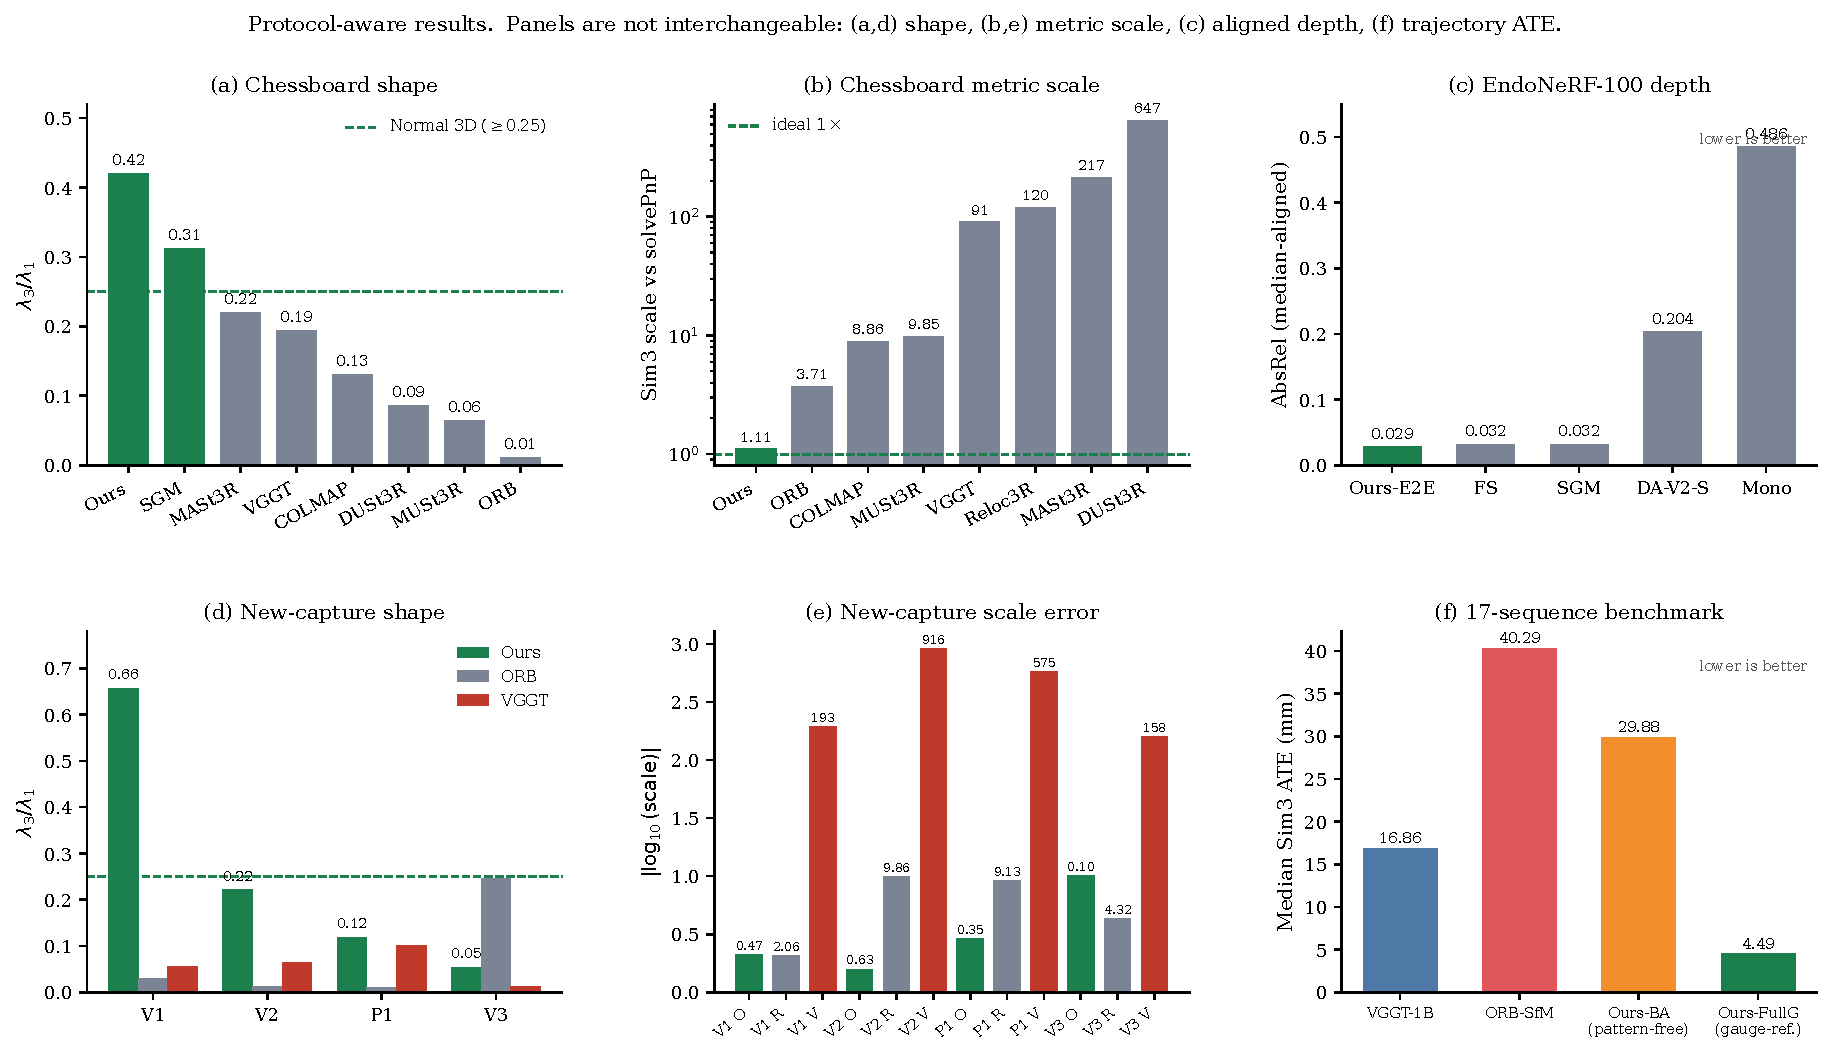
\includegraphics[width=\linewidth]{fig_sota_summary.pdf}
\caption{Protocol-aware graphical summary corresponding to Table~\ref{tab:sota_summary}.\
(a)~Chessboard 3D shape ratio: only Ours ($0.42$) and Stereo SGM ($0.31$) exceed the Normal\,3D threshold ($0.25$, dashed).\
(b)~Chessboard metric scale (log): Ours recovers $1.11\times$; all baselines drift by $3.7\times$--$647\times$.\
(c)~EndoNeRF-100 depth (median-aligned AbsRel): the calibrated variant ($0.0285$) leads FoundationStereo ($0.0321$) and Stereo SGM ($0.0323$).\
(d)~New-capture shape: Ours reaches the best geometry on three of four sequences and the only Normal\,3D (V1).\
(e)~New-capture scale error $|\log_{10}\mathrm{scale}|$: Ours stays within ${\approx}2\times$ on V1--V2 while VGGT drifts by $158\times$--$916\times$.\
(f)~17-sequence median ATE: the gauge-referenced mode reaches the $4.49$\,mm pattern floor; pattern-free Ours-BA ($29.88$\,mm) lies between VGGT-1B ($16.86$\,mm) and ORB-SfM ($40.29$\,mm).\
Panels measure different quantities under different protocols and are not interchangeable.}
\label{fig:sota_summary}
\end{figure*}

Fig.~\ref{fig:sota_summary} visualises the same headline numbers graphically, with each panel labelled by its protocol.

\section{Discussion}
\label{sec:discussion}

\paragraph{Why feed-forward networks fail on endoscopic data.}
The domain gap between Internet-scale natural-image training sets and endoscopic imaging causes two specific failures: (1)~specular reflections and smooth tissue provide few reliable features, breaking correspondence estimation; (2)~repetitive patterns (e.g., calibration grids, tissue textures) confuse learned matching priors, leading to incorrect depth ordering and collapsed 3D structure.
Our method mitigates both through gradient-based heightfield construction (uniform specular responses are suppressed by percentile truncation) and the ROI mask (constraining reconstruction to geometrically reliable regions); the same heightfield geometry is also the substrate on which inter-frame poses are estimated, so reliable localization and reliable correspondences share a common 3D signal that 2D-only or learned-natural-image methods lack.
Across the chessboard, public stereo sets, and the newly captured sequences, no feed-forward method achieves $\lambda_3/\lambda_1 \geq 0.25$ on any sequence tested.

\paragraph{Generalization across imaging hardware.}
The stereo laparoscopic evaluation (Section~\ref{sec:stereo_lap}) demonstrates that our method generalizes across five different endoscope configurations (focal lengths 383--766\,px, resolutions $360\times288$ to $720\times576$) without re-tuning, achieving depth accuracy identical to stereo SGM while providing an additional heightfield confidence map.
This hardware-agnostic behavior stems from the gradient-based design: percentile truncation adapts automatically to the gradient distribution of each frame, making the heightfield independent of absolute image intensity or resolution.

\paragraph{Implications for imaging, visualization, and image-guided intervention.}
From an imaging-and-graphics standpoint, the useful output is not a disparity map alone but a surface that can be inspected, overlaid, and measured.
The point cloud---whose poses are estimated from the heightfield rather than supplied externally---can be rendered and overlaid. A lesion-diameter or standoff measurement is not supported by the present square-size error: on the $5.0$\,mm board the native mean absolute edge error is $10.9$\,mm (Section~\ref{sec:spacing}). Overlay and measurement both fail when the cloud collapses to a cone or plane.
Relative to electromagnetic tracking (sensor coils, metal interference) and intra-operative CT or ultrasound (added hardware or dose), a vision-only pipeline that reuses the existing endoscope feed adds no device to the sterile field.
The present validation is computational rather than clinical: it uses ex-vivo porcine tissue (SCARED), de-identified surgical recordings (EndoNeRF), and a bench-top chessboard phantom, with no live patients or prospective surgical use.
The chessboard Normal\,3D result requires a sufficiently strong heightfield signal; the ablation in Section~\ref{sec:results} shows that a 2D pose front-end collapses the cloud, so immediate deployment is limited to settings with adequate texture and viewing geometry (calibrated bench-top and stereo-laparoscopic sequences) rather than arbitrary marker-free footage.
Marker-free masks via instrument and tissue segmentation, and a prospective phantom or cadaver study against electromagnetic tracking, are the natural next steps toward clinical translation.

\paragraph{Limitations.}
First, the default ROI is a landmark hull or a contour fallback; on the new sequences the board is visible on only $12$--$28\%$ of frames, so a semantic tissue mask (Section~\ref{sec:pseudo3d}) is the intended replacement rather than a second reconstruction primitive.
Second, the 2.5-D heightfield cannot represent occlusions or multiple depth layers, and degrades when scene motion is predominantly lateral (Section~\ref{sec:endonerf}). Instruments must be masked out, not lifted as a second surface.
Third, pairwise heightfield-ICP accumulates drift on long, weakly anchored sequences (V3: scale $0.099{\times}$, $\lambda_3/\lambda_1{=}0.053$, ATE $38.8$\,mm). The 7-D matches were not archived, so that residual was not rerun on the published cloud. A pose-only substitute re-estimated every fourth relative pose by Kabsch on high-gradient heightfield vertices and reintegrated the chain. On the 27 frames of that stride that meet the PnP reference, Sim3 scale moved from $0.090$ to $0.081$ and ATE from $35.7$\,mm to $33.6$\,mm. Scale did not approach $1$. The published full-sequence figures are unchanged.
Fourth, reconstruction remains confined to $M_t$; a soft semantic mask would enlarge coverage without changing the heightfield equations.
Fifth, orientation in the heightfield embedding is only approximate. Translation and scale are reliable on the chessboard (ATE $3.89$\,mm, scale $1.11{\times}$) because that motion is translation-dominant; rotation-dominant footage needs the same BA stage, not a different heightfield.
Sixth, the gauge-referenced mode (Ours-FullGauge) reports per-frame pattern poses: it characterises the metric accuracy the gauge injects when a fiducial is fully visible, and is not a visual-tracking result. Pattern-free visual tracking is reported separately (Ours-BA), where VGGT-1B remains ahead on average ($18.10$\,mm vs.\ $35.52$\,mm mean ATE) and our advantage is confined to the smoke/deformation regime (e.g., \texttt{s10097}) and to metric scale fidelity.
A detailed analysis of failure cases is provided in the Supplementary Material, Section~F.3.

% ======================================================================
%  Section 6: Conclusion
% ======================================================================
\section{Conclusion}
\label{sec:conclusion}

We have presented a pseudo-3D heightfield framework that turns monocular endoscopic video into a 3D surface that is both displayable and measurable. The heightfield serves two roles at once: it is the geometric matching substrate on which frames are registered, densely matched, and bundle-adjusted over a multi-stride co-visibility graph, and it is the operator corrector whose physical normal field vetoes the spurious homography branch while a calibration gauge injects true metric scale.
The framework offers dual operating modes: a lightweight, CPU-only classical variant for resource-constrained clinical systems, and a GPU-accelerated multi-stride BA variant for high-precision global trajectory optimization.
On the endoscopic chessboard benchmark the heightfield is the only reconstruction that stays Normal\,3D ($\lambda_3/\lambda_1 = 0.42$) with near-ideal metric scale ($1.11\times$), where every feed-forward and SfM baseline collapses or drifts.
On a newly established 17-sequence surgical video benchmark, the pattern-free multi-view BA outperforms the classical ORB-SfM baseline ($35.52$\,mm vs.\ $43.72$\,mm mean ATE) and beats VGGT-1B on the smoke-filled cavity \texttt{s10097} ($24.86$\,mm vs.\ $37.25$\,mm); when the calibration gauge is visible, the gauge-referenced trajectory reaches the pattern-localisation floor of $4.49$\,mm median ATE.
Furthermore, on the public EndoNeRF benchmark, our calibrated stereo variant reaches an overall AbsRel of $0.0285$ (FoundationStereo $0.0321$).
These results establish a dependable pathway from monocular endoscopic video to un-collapsed, metrically anchored 3D surfaces for surgical visualization and quantitative intra-operative measurement.

\section*{Acknowledgements}
The authors thank the developers of the SCARED~\cite{allan2021stereo} and EndoNeRF~\cite{wang2022endonerf} datasets for making their data publicly available, which made the cross-dataset evaluation possible.

\section*{Declarations}

\paragraph{Funding.}
This work was supported by the National Natural Science Foundation of China (Grant No.~6240074117); the Natural Science Project of the Science and Technology Department of Henan Province (Grant Nos.~232102211001, 232102210042, 232102210005, 222102310058); the Open Project Program of the State Key Laboratory of Virtual Reality Technology and Systems (Grant No.~VRLAB2023C03); the High-level Talents Fund of Henan University of Technology (Grant Nos.~2022BS076, 2022BS075); and the Cultivation Project of Tuoxin Team in Henan University of Technology (Grant No.~2024TXTD18).

\paragraph{Conflict of interest.}
The authors declare that they have no known competing financial interests or personal relationships that could have appeared to influence the work reported in this paper.

\paragraph{Ethics statement.}
This study uses public datasets and in-house bench-top phantom recordings. The SCARED dataset~\cite{allan2021stereo} contains ex-vivo porcine cadaver tissue and does not involve human subjects. The EndoNeRF dataset~\cite{wang2022endonerf} consists of de-identified surgical recordings previously released by the original authors under their own institutional ethics approval; the present study is a secondary computational analysis of these public recordings and did not require additional ethical clearance. The in-house endoscopic chessboard, stereo-laparoscopic, and newly captured monocular sequences are bench-top phantom recordings and contain no patient-identifiable information.

\paragraph{Authors' contributions.}
\textbf{Ranyang Li:} Conceptualization, Methodology, Software, Validation, Formal analysis, Investigation, Data curation, Writing -- original draft, Visualization, Funding acquisition. \textbf{Wufeng Liu:} Methodology, Validation, Writing -- review \& editing. \textbf{Xiaodong Guo:} Software, Validation, Data curation. \textbf{Nan Wei:} Resources, Supervision. \textbf{Chao Fan:} Software, Investigation. All authors read and approved the final manuscript.

\paragraph{Data availability.}
Public datasets are cited at their original sources: SCARED~\cite{allan2021stereo} and EndoNeRF~\cite{wang2022endonerf}. Evaluation scripts, the pipeline of record, result JSONs, and the figures used in this manuscript are at \url{https://github.com/liranyang123456-commits/re3d-heightfield}. In-house sequences and trained stereo-variant weights will be deposited in the same repository; until the full data release they remain available from the corresponding author upon reasonable request. The random seed used for PCA sub-sampling is 42.

\paragraph{Declaration of generative AI and AI-assisted technologies in the manuscript preparation process.}
During the preparation of this work the authors used generative-AI tools solely for language polishing of author-written text. After using these tools, the authors reviewed and edited the content as needed and take full responsibility for the content of the published article.


% ── References (BibTeX) ──
\bibliography{references}

\end{document}
